\باب{ساکن مقناطیسی میدان}
برقی میدان کا منبع برقی بار ہے جس پر باب \حوالہ{باب_کولمب_قانون} میں تفصیل سے بات کی گئی۔مقناطیسی میدان کا منبع یا تو مقناطیس ہو سکتا ہے، یا وقت کے ساتھ بدلتا برقی میدان اور یا پھر برقی رو۔اس کتاب میں مقناطیس سے پیدا ہونے والے مقناطیسی میدان پر غور نہیں کیا جائے گا۔وقت کے ساتھ بدلتے برقی میدان سے پیدا مقناطیسی میدان پر ایک اور باب میں غور کیا جائے گا جبکہ اس باب میں برقی رو سے پیدا ساکن مقناطیسی میدان پر غور کیا جائے گا۔

\حصہ{بایوٹ-سیوارٹ کا قانون}
برقی رو اور اس سے پیدا مقناطیسی میدان کا تعلق \اصطلاح{بایوٹ-سیوارٹ}\فرہنگ{بایوٹ-سیوارٹ}\حاشیہب{Biot-Savart law}\فرہنگ{Biot-Savart law} کا قانون\حاشیہد{یہ قانون فرانس کے  بایوٹ اور سیوارٹ نے 1820 میں پیش کیا۔یہ دونوں ایمپیئر کے ساتھی تھے۔}
\begin{align}\label{مساوات_بایوٹ_سیوارٹ_تفرق_شکل}
\dif \kvec{H}=\frac{I \dif \kvec{L} \times \aR}{4 \pi R^2}
\end{align}
 بیان کرتا ہے جہاں سے مقناطیسی شدت \عددیء{\kvec{H}} کی اکائی ایمپیئر فی میٹر \عددیء{(\si{\ampere \per \meter})} حاصل ہوتی ہے۔آئیں شکل \حوالہ{شکل_مقناطیسی_بایوٹ_سیوارٹ_قانون} کی مدد سے  اس قانون کا مطلب سمجھیں۔

\begin{figure}
\centering
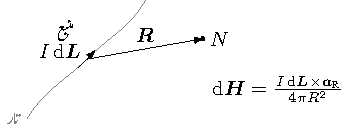
\includegraphics{figMagneticBiotSavartDefinedBasic}
\caption{بایوٹ سیوارٹ کا قانون۔}
\label{شکل_مقناطیسی_بایوٹ_سیوارٹ_قانون}
\end{figure}
یہ قانون باریک تار کی انتہائی چھوٹی لمبائی \عددیء{\dif \kvec{L}} جس میں  برقی رو \عددیء{I} گزر رہی ہو کی وجہ  سے  نقطہ \عددیء{N} پر پیدا سمتی برقی میدان \عددیء{\kvec{H}} دیتا ہے۔نقطہ \عددیء{N} باریک تار کے چھوٹے حصے سے \عددیء{\kvec{R}} فاصلے پر ہے۔باریک تار سے مراد ایسی ٹھوس نلکی نما موصل تار ہے جس کی موٹائی کم سے کم ہو۔چھوٹی لمبائی \عددیء{\dif \kvec{L}} کی سمت برقی رو کی سمت میں ہے اور \عددیء{I \dif \kvec{L}}  مقناطیسی میدان کا منبع ہے۔

مقناطیسی شدت کی قیمت برقی رو ضرب باریک چھوٹی تار کی لمبائی \عددیء{I \dif \kvec{L}} اور \عددیء{\aR} کے سمتی ضرب کے برائے راست تناسب جبکہ ان کے مابین فاصلہ \عددیء{R} کے مربع کے بالعکس تناسب رکھتی ہے۔تناسبی مستقل \عددیء{\tfrac{1}{4\pi}} ہے۔

بایوٹ-سیوارٹ کے  قانون کا موازنہ کولمب کے قانون کے ساتھ کرنے کی غرض سے دونوں مساوات کو ایک ساتھ لکھتے ہیں۔
\begin{gather}
\begin{aligned}\label{مساوات_بایوٹ_سیوارٹ_تفرق_شکل_ب}
\dif \kvec{H}_2&=\frac{I_1 \dif \kvec{L}_1 \times \kvec{a}_{R21}}{4 \pi R_{21}^2}\\
\dif \kvec{E}_2&=\frac{\dif Q_1 \kvec{a}_{R21}}{4\pi \epsilon_0 R_{21}^2}
\end{aligned}
\end{gather}
ان مساوات میں زیر نوشت میں \عددیء{2} اس مقام کو ظاہر کرتی ہے جہاں میدان کی قیمت حاصل کی گئی ہے جبکہ زیر نوشت میں \عددیء{1} میدان کے منبع کے مقام کو ظاہر کرتی ہے۔دونوں میدان فاصلے کے مربع کا بالعکس تناسب رکھتے ہیں۔دونوں اقسام کے میدان کی شدت اور میدان کی منبع کا خطی تعلق ہے۔دونوں میں فرق میدان کی سمت کا ہے۔برقی میدان کی سمت منبع سے اس نقطہ کی جانب ہے جس پر میدان حاصل کیا جا رہا ہو۔مقناطیسی میدان کی سمت سمتی ضرب کے دائیں ہاتھ کے قانون سے حاصل ہوتی ہے۔

شکل \حوالہ{شکل_مقناطیسی_تار_کا_ٹکڑا_اور_میدان} میں تار کے چھوٹے حصے \عددیء{\dif l} سے نقطہ \عددیء{N} پر مقناطیسی میدان کی مقدار
\begin{align}\label{مساوات_مقناطیسی_تار_کا_ٹکڑا_اور_میدان}
\dif H=\frac{I \dif l \sin \theta}{4\pi r^2}
\end{align}
ہو گا۔

\begin{figure}
\centering
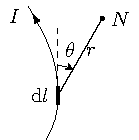
\includegraphics{figMagneticSectionOfWire}
\caption{تار کے چھوٹے حصے سے پیدا میدان۔}
\label{شکل_مقناطیسی_تار_کا_ٹکڑا_اور_میدان}
\end{figure}
بایوٹ-سیوارٹ کے قانون کو مساوات \حوالہ{مساوات_بایوٹ_سیوارٹ_تفرق_شکل} کی شکل میں تجرباتی طور پر ثابت نہیں کیا جا سکتا چونکہ باریک تار کی چھوٹی لمبائی میں برقی رو تب گزرے گی جب برقی رو اس چھوٹی تار تک پہنچائی جائے۔جو تار اس تک برقی رو پہنچائے گی، وہ بھی مقناطیسی میدان پیدا کرے گی۔انہیں علیحدہ علیحدہ نہیں کیا جا سکتا۔ہم فی الحال صرف یک سمتی برقی رو کی بات کر رہے ہیں۔ یک سمتی برقی رو کی صورت میں وقت کے ساتھ حجمی کثافتِ بار تبدیل نہیں ہو گا لہٰذا صفحہ \حوالہصفحہ{مساوات_کپیسٹر_استمراری_مساوات_نقطہ_شکل} پر دئے  استمراری مساوات
\begin{align*}
\nabla \cdot \kvec{J}=-\frac{\partial \rho_h}{\partial t}
\end{align*}
سے
\begin{align}\label{مساوات_مقناطیسی_صرف_مکمل_بند_راہ}
\nabla \cdot \kvec{J}=0
\end{align}
حاصل ہو گا جسے مسئلہ پھیلاو کی مدد سے
\begin{align*}
\oint_S  \kvec{J} \cdot \dif \kvec{S}=0
\end{align*}
لکھا جا سکتا ہے۔یہ مساوات کہتی ہے کہ کسی بھی بند سطح سے گزرتی ہوئی برقی رو صفر کے برابر ہے۔یہ صرف اس صورت ممکن ہے جب برقی رو کسی بند راہ پر گزر رہی ہو۔ہمیں ایسی ہی مکمل بند راہ کے برقی رو کے اثر کو دیکھنا ہو گا نا کہ تار کے کسی چھوٹے حصے  کے برقی رو کو۔ 

یوں بایوٹ-سیوارٹ قانون کی تکمل شکل
\begin{align}\label{مساوات_بایوٹ_سیوارٹ_تکمل_شکل}
\kvec{H}=\oint \frac{I \dif \kvec{L} \times \aR}{4 \pi R^2}
\end{align}
ہی تجرباتی طور پر ثابت کی جا سکتی ہے۔

مساوات \حوالہ{مساوات_بایوٹ_سیوارٹ_تفرق_شکل} سے مساوات \حوالہ{مساوات_بایوٹ_سیوارٹ_تکمل_شکل} لکھی جا سکتی ہے۔البتہ مساوات \حوالہ{مساوات_بایوٹ_سیوارٹ_تکمل_شکل} میں تکمل کے اندر کوئی بھی ایسی اضافی تفاعل شامل کیا جا سکتا ہے جس کا بند تکمل صفر کے برابر ہو۔مقداری میدان کا ڈھلوان ہر صورت بقائی میدان ہوتا ہے لہٰذا مساوات \حوالہ{مساوات_بایوٹ_سیوارٹ_تکمل_شکل} میں \عددیء{\nabla G} کے شمول سے اس کے جواب میں کوئی فرق نہیں پڑے گا۔\عددیء{G} کوئی بھی مقداری میدان ہو سکتا ہے۔

واضح رہے کہ کسی بھی نقطے پر مقناطیسی میدان مکمل برقی دور کے اثر کو شامل کرنے سے ہی حاصل کیا جا سکتا ہے۔برقی رو گزارتی تار کے کچھ حصے کے میدان یا ایسے میدان سے پیدا قوت کی بات بے معنی ہو گی۔

\begin{figure}
\centering
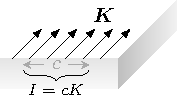
\includegraphics{figMagneticInfiniteSurfaceCurrentDensity}
\caption{سطحی کثافت برقی رو کے $c$ چوڑائی میں کل $cK$ برقی رو ہو گا۔}
\label{شکل_مقناطیسی_سطحی_کثافت_برقی_رو_اور_رو}
\end{figure}

شکل \حوالہ{شکل_مقناطیسی_سطحی_کثافت_برقی_رو_اور_رو} میں یکساں سطحی کثافت برقی رو \عددیء{\kvec{K}} دکھایا گیا ہے۔سطحی کثافت برقی رو کو ایمپیئر فی اکائی چوڑائی پیش کیا جاتا ہے لہٰذا \عددیء{c} چوڑائی کے حصے میں
\begin{align*}
I=cK
\end{align*}
 برقی رو ہو گا۔اگر کثافت برقی رو یکساں نہ ہو تب کسی بھی چوڑائی میں کل برقی رو بذریعہ تکمل
\begin{align*}
I=\int K \dif c
\end{align*}
حاصل ہو گی جہاں \عددیء{\dif c} چوڑائی کا چھوٹا حصہ ہے۔یوں \عددیء{\dif \kvec{L}} کو سطحی کثافت برقی رو \عددیء{\kvec{K}} یا حجمی کثافت برقی رو \عددیء{\kvec{J}} کی صورت میں
\begin{align}\label{مساوات-مقناطیسی_تفرقی_برقی_رو_مختلف_صورت}
I \dif \kvec{L}=\kvec{K} \dif S=\kvec{J} \dif h
\end{align}
لکھا جا سکتا ہے۔یوں بایوٹ-سیوارٹ کے قانون کو
\begin{align}
\kvec{H}=\int_S \frac{\kvec{K} \times \aR \dif S}{4\pi R^2}
\end{align}
یا
\begin{align}
\kvec{H}=\int_h \frac{\kvec{J} \times \aR \dif h}{4\pi R^2}
\end{align}
لکھا جا سکتا ہے۔

\begin{figure}
\centering
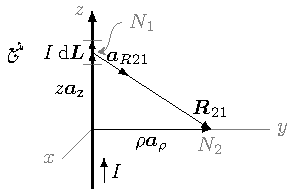
\includegraphics{figMagneticInfiniteStraightWiresField}
\caption{سیدھی لامحدود تار سے پیدا مقناطیسی میدان}
\label{شکل_مقناطیسی_سیدھی_لامحدود_تار_کا_میدان}
\end{figure}
آئیں  سیدھی  لامحدود لمبائی کی تار جس میں سے برقی رو گزر رہی ہو کی مقناطیسی میدان بایوٹ-سیوارٹ کے قانون سے حاصل کریں۔شکل \حوالہ{شکل_مقناطیسی_سیدھی_لامحدود_تار_کا_میدان} میں صورت حال دکھائی گئی ہے۔اس تار کے دونوں سرے لامحدود فاصلے پر ہیں۔تار کے قریب نقطہ \عددیء{N_2} پر مقناطیسی میدان کا بیشتر حصہ تار کے اس حصے کی وجہ سے ہو گا جو \عددیء{N_2} کے قریب ہو۔یوں لامحدود فاصلے پر تار کے سروں تک برقی رو پہنچانے  والی تار کا نقطہ \عددیء{N_2} پر اثر کو نظرانداز کرتے ہوئے آگے بڑھتے ہیں۔ 

نقطہ \عددیء{N_1} پر تار کے چھوٹے حصے \عددیء{\dif \kvec{L}} میں برقی رو کو منبع مقناطیسی میدان تصور کرتے ہوئے مساوات \حوالہ{مساوات_بایوٹ_سیوارٹ_تفرق_شکل} کی مدد سے نقطہ \عددیء{N_2} پر مقناطیسی میدان لکھا جا سکتا ہے۔چونکہ 
\begin{align*}
\kvec{R}_{21}=\rho \arho-z \az
\end{align*}
کے برابر ہے لہٰذا
\begin{align*}
R_{21}&=\abs{\kvec{R}_{21}}=\sqrt{\rho^2+z^2}\\
\aR&=\frac{\kvec{R}_{21}}{\abs{\kvec{R}_{21}}}=\frac{\rho \arho-z \az}{\sqrt{\rho^2+z^2}}
\end{align*}
لکھے جا سکتے ہیں۔نلکی محدد میں چھوٹی لمبائی
\begin{align*}
\dif \kvec{L}=\dif \rho \arho+\rho \dif \phi \aphi+\dif z \az
\end{align*}
لکھی جاتی ہے۔چونکہ یہاں \عددیء{\dif \rho=0} اور \عددیء{\dif \phi=0} ہیں لہٰذا \عددیء{\dif \kvec{L}=\dif z \az} لکھتے ہوئے  مساوات \حوالہ{مساوات_بایوٹ_سیوارٹ_تفرق_شکل} کو
\begin{align*}
\dif \kvec{H}_2=\frac{I \dif z \az \times (\rho \arho -z\az)}{4 \pi (\rho^2+z^2)^{\frac{3}{2}}}
\end{align*}
لکھا جا سکتا ہے۔پورے تار کا مقناطیسی میدان اس مساوات کے تکمل سے حاصل ہو گا جہاں تکمل\عددیء{-\infty} تا \عددیء{+\infty} حاصل کیا جائے گا۔اس طرح
\begin{align*}
\kvec{H}_2&=\int_{-\infty}^{\infty}\frac{I \dif z \az \times (\rho \arho -z\az)}{4 \pi (\rho^2+z^2)^{\frac{3}{2}}}\\
&=\frac{I \rho}{4\pi}\int_{-\infty}^{\infty} \frac{\aphi \dif z }{(\rho^2+z^2)^{\frac{3}{2}}}
\end{align*}    
لکھا جا سکتا ہے جہاں صفحہ \حوالہصفحہ{مساوات_سمتیات_نلکی_اکائی_سمتیات_کا_سمتی_ضرب} پر مساوات \حوالہ{مساوات_سمتیات_نلکی_اکائی_سمتیات_کا_سمتی_ضرب} کی مدد سے \عددیء{\az \times \arho=\aphi} جبکہ مساوات \حوالہ{مساوات_سمتیات_نلکی_اکائی_سمتیات_کا_سمتی_ضرب_ب} کی مدد سے \عددیء{\az \times \az=0} لکھے گئے ہیں۔

مندرجہ بالا مساوات میں تکمل کے اندر \عددیء{\aphi} پر نظر رکھنی ہو گی۔اگرچہ \عددیء{\aphi} اکائی سمتیہ ہے لہٰذا اس کی لمبائی تبدیل نہیں ہو سکتی البتہ یہ دیکھنا ضروری ہے کہ آیا تکمل کا متغیرہ یعنی \عددیء{z} تبدیل کرنے سے \عددیء{\aphi} کی سمت تو تبدیل نہیں ہوتی۔صفحہ \حوالہصفحہ{مساوات_سمتیہ_اکائی_زاویہ_کارتیسی_میں} پر مساوات \حوالہ{مساوات_سمتیہ_اکائی_زاویہ_کارتیسی_میں} کے تحت
\begin{align*}
\aphi&=-\frac{y}{\sqrt{x^2+y^2}} \ax+\frac{x}{\sqrt{x^2+y^2}} \ay
\end{align*}
لکھا جا سکتا ہے۔آپ دیکھ سکتے ہیں کہ \عددیء{z} تبدیل کرنے سے \عددیء{\aphi} پر کوئی اثر نہیں پڑتا لہٰذا \عددیء{\aphi} کو تکمل کے باہر منتقل کیا جا سکتا ہے۔یوں
\begin{gather}
\begin{aligned}\label{مساوات_مقناطیسی_سیدھی_لامحدود_تار_کا_میدان}
\kvec{H}_2&=\frac{I \rho\aphi}{4\pi}\int_{-\infty}^{\infty} \frac{\dif z }{(\rho^2+z^2)^{\frac{3}{2}}}\\
&=\eval{\frac{I \rho \aphi}{4\pi} \frac{z}{\rho^2 \sqrt{\rho^2+z^2}}}_{-\infty}^{+\infty}
\end{aligned}
\end{gather}    
سے
\begin{align}
\kvec{H}_2=\frac{I}{2\pi \rho} \aphi
\end{align}
حاصل ہوتا ہے۔شکل \حوالہ{شکل_مقناطیسی_سیدھے_تار_کا_میدان_دائرے} میں برقی رو صفحہ سے باہر نکل رہی ہے جبکہ گول دائرے مقناطیسی میدان کو ظاہر کرتے ہیں۔اگر تار کو دائیں ہاتھ سے یوں پکڑا جائے کہ انگوٹھا برقی رو کی سمت میں ہو تب اس ہاتھ کی انگلیاں تار کے گرد مقناطیسی میدان کی سمت میں لپٹی ہوں گی۔آپ دیکھ سکتے ہیں کہ یہ مقناطیسی میدان نا تو \عددیء{z} تبدیل کرنے اور نا ہی زاویہ \عددیء{\phi} تبدیل کرنے سے تبدیل ہوتا ہے۔اس کی قیمت صرف تار سے فاصلے پر منحصر ہے۔
\begin{figure}
\centering
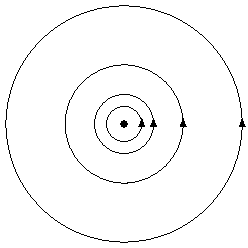
\includegraphics{figMagneticInfiniteStraightWiresStreamlines}
\caption{سیدھی لمبی تار کا مقناطیسی میدان تار کے گرد دائرے بناتا ہے۔برقی رو صفحے سے باہر نکل رہی ہے۔}
\label{شکل_مقناطیسی_سیدھے_تار_کا_میدان_دائرے}
\end{figure}
%
\begin{figure}
\centering
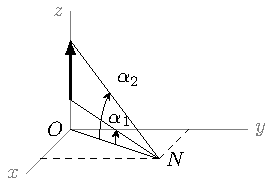
\includegraphics{figMagneticStraightWiresField}
\caption{سیدھی  محدود لمبائی کے تار کی مقناطیسی شدت۔}
\label{شکل_مقناطیسی_سیدھے_محدود_تار_کا_میدان}
\end{figure}

اگر شکل \حوالہ{شکل_مقناطیسی_سیدھی_لامحدود_تار_کا_میدان} میں تار لامحدود نہ ہو تب مساوات \حوالہ{شکل_مقناطیسی_سیدھے_محدود_تار_کا_میدان} میں تکمل کے محدود حدود پر کرنے سے مقناطیسی میدان کی شدت
\begin{align}\label{مساوات_مقناطیسی_محدود_تار_کی_مقناطیس}
\kvec{H}=\frac{I}{4\pi \rho} \left(\sin \alpha_2-\sin \alpha_1 \right) \aphi
\end{align}
حاصل ہوتی ہے جہاں شکل \حوالہ{شکل_مقناطیسی_سیدھے_محدود_تار_کا_میدان} میں \عددیء{\alpha_1} اور \عددیء{\alpha_2} کی نشاندہی کی گئی ہے۔تار کا نچلا سرا \عددیء{xy} سطح یعنی \عددیء{z=0} سطح سے نیچے ہونے کی صورت میں \عددیء{\alpha_1} کی قیمت منفی ہو گی۔یہی کچھ تار کے دوسرے سرے اور \عددیء{\alpha_2} کے لئے بھی درست ہے۔

\حصہ{ایمپیئر کا دوری قانون}
کولمب کے قانون کی مدد سے مختلف طرز پر پائے جانے والے بار کے برقی میدان حاصل کرنے کے بعد ہم نے گاوس کا قانون اخذ کیا جس سے ہماری زندگی نہایت آسان ہو گئی۔گاوس کے قانون کی مدد سے متشاکل بار سے پیدا برقی میدان انتہائی آسانی سے حاصل ہوتا ہے۔متشاکل برقی رو کے مقناطیسی میدان حاصل کرنے کا بھی اتنا ہی آسان طریقہ موجود ہے جسے \اصطلاح{ایمپیئر کا دوری قانون}\فرہنگ{ایمپیئر کا دوری قانون}\حاشیہب{Ampere's circuital law}\فرہنگ{Ampere's circuital law} کہتے ہیں۔اس قانون کو بایوٹ-سیوارٹ کے قانون سے حصہ \حوالہ{حصہ_ایمپیئر_کا-دوری_قانون} میں حاصل کیا گیا ہے۔فی الحال ہم اس قانون کو استعمال کرنا سیکھتے ہیں۔اس قانون کے استعمال کے وقت مسئلے پر غور کرتے ہوئے بغیر حساب و کتاب کے فیصلہ کیا جاتا ہے کہ مقناطیسی میدان کے کون کون سے اجزاء موجود نہیں ہونے چاہئے۔یہ فیصلہ برقی رو کے راستے کو دیکھ کر کیا جاتا ہے۔

ایمپیئر کا دوری قانون کہتا ہے کہ یک سمتی برقی رو کے گرد کسی بھی راہ \عددیء{\kvec{H}} کا لکیری بند تکمل گھیرے برقی رو کے برابر ہو گا یعنی
\begin{align}\label{مساوات_مقناطیسی_ایمپیئر_کا_دوری_قانون}
\oint \kvec{H} \cdot \dif \kvec{L}=I
\end{align}

لکیری بند تکمل کی سمت میں برقی رو کے گرد  دائیں ہاتھ کی انگلیاں گھمانے سے اسی ہاتھ کا انگوٹھا مثبت برقی رو کی سمت دے گا۔ایسا کرتے وقت انگوٹھے کو باقی چار انگلیوں کے عمودی رکھا جاتا ہے۔

کسی بھی راہ \عددیء{\kvec{H}} کے لکیری تکمل سے مراد اس راہ  کو انتہائی چھوٹے چھوٹے ٹکڑوں \عددیء{\dif \kvec{L}} میں تقسیم کر کے ہر ٹکڑے پر \عددیء{\kvec{H}} کی قیمت استعمال کرتے ہوئے \عددی{\kvec{H} \cdot \dif \kvec{L}} حاصل کر کے تمام \عددی{\kvec{H} \cdot \dif \kvec{L}} کا مجموعہ حاصل کرنا ہے۔مقناطیسی شدت \عددیء{\kvec{H}} کی قیمت مختلف مقامات پر عموماً مختلف ہو گی۔یوں کسی ایک نقطے پر \عددی{\kvec{H} \cdot \dif \kvec{L}} کی قیمت کسی دوسرے نقطے کے \عددی{\kvec{H} \cdot \dif \kvec{L}} سے مختلف ہو گی۔ایمپیئر کا دوری قانون کہتا ہے کہ اگرچہ یک سمتی برقی رو کے گرد دو مختلف بند راہوں پر جگہ جگہ \عددی{\kvec{H} \cdot \dif \kvec{L}} کی قیمتیں مختلف ہوں گی لیکن دونوں راہ پر ان کا مجموعہ عین برقی رو کے برابر ہو گا۔

کسی بھی سطح کا محیط، بند راہ ہوتی ہے۔اسی طرح کوئی بھی بند راہ، لامحدود سطحوں کا محیط ہوتا ہے۔یوں بند راہ کا گھیرا ہوا برقی رو ان تمام سطحوں کو چھیرتا ہوا گزرے گا جن کا محیط یہ بند راہ ہو۔

گاوس کے قانون کا استعمال تب ممکن ہوتا ہے جب بند سطح میں کل برقی بار معلوم ہو۔ایمپیئر کا دوری قانون اس صورت استعمال کیا جا سکتا ہے جب  بند راہ میں گھیرا کل یک سمتی برقی رو معلوم ہو۔   

آئیں شکل \حوالہ{شکل_مقناطیسی_سیدھی_لامحدود_تار_کا_میدان} میں دکھائے گئے  برقی رو گزارتے سیدھی لامحدود لمبائی کے تار کی مقناطیسی شدت ایمپیئر کے دوری قانون یعنی مساوات \حوالہ{مساوات_مقناطیسی_ایمپیئر_کا_دوری_قانون} کی مدد سے دوبارہ حاصل کریں۔اس مساوات کو استعمال کرتے ہوئے  برقی رو کے گرد راہ یوں چننی جاتی ہے کہ اس پر \عددیء{\kvec{H}} اور \عددیء{\dif \kvec{L}} یا تو آپس میں عمودی ہوں اور یا \عددیء{\kvec{H}} کی قیمت قطعی اور اس کی سمت \عددیء{\dif \kvec{L}} کے متوازی ہو۔پہلی صورت میں دونوں متغیرات کے مابین نوے درجے کا زاویہ  ہے اور \عددیء{\cos 90\degree=0} ہوتا ہے لہٰذا \عددیء{\kvec{H} \cdot \dif \kvec{L}} صفر کے برابر ہو گا اور یوں راہ کے اس حصے پر تکمل صفر کے برابر ہو گا۔ دوسری صورت میں متغیرات کے مابین صفر درجے کا زاویہ ہے اور \عددیء{\cos 0 \degree=1} ہوتا ہے لہٰذا \عددیء{\kvec{H} \cdot \dif \kvec{L}}  کو \عددیء{H \dif L} لکھا جا سکتا ہے اور ساتھ ہی ساتھ مقناطیسی شدت کی قیمت قطعی ہونے کی وجہ سے \عددیء{H} کو تکمل کے باہر لے جایا جا سکتا ہے۔یوں راہ کے اس راستے پر تکمل کی قیمت \عددیء{H L} کے برابر ہو گی جہاں \عددیء{L} راہ کے اس حصے کی لمبائی ہے۔

تار کے گرد اور اس کے ساتھ ساتھ حرکت کرنے سے واضح ہوتا ہے کہ مسئلے کی نوعیت نا تو تار کے گرد زاویہ \عددیء{\phi} پر اور نا ہی محدد \عددیء{z} پر منحصر ہے۔تار سے دور یا اس کے قریب ہونے سے ہی مسئلے کی نوعیت میں تبدیلی آتی ہے۔یوں صاف ظاہر ہے کہ مقناطیسی شدت صرف \عددیء{\rho} پر منحصر ہو سکتی ہے۔اسی طرح بایوٹ-سیوارٹ کے قانون کو مد نظر رکھتے ہوئے ہم دیکھ سکتے ہیں کہ مقناطیسی شدت \عددیء{\aphi} سمت رکھتی ہے یعنی اس کا صرف \عددیء{H_{\phi}} جزو پایا جائے گا۔یوں اگر \عددیء{\rho} تبدیل کئے بغیر تار کے گرد چلا جائے تو ہم یقین رکھ سکتے ہیں کہ \عددیء{\kvec{H}} کی حتمی قیمت \عددیء{H_{\phi}} تبدیل نہیں ہو گی۔ساتھ ہی ساتھ اس راہ پر کسی بھی نقطے پر  \عددیء{\dif \kvec{L}=\rho \dif \phi \aphi} اور \عددیء{H_{\phi} \aphi} آپس میں متوازی ہوں گے لہٰذا ایمپیئر کے دوری قانون سے
\begin{align*}
\oint \kvec{H} \cdot \dif \kvec{L}=\int_0^{2\pi} H_{\phi} \rho \dif \phi=H_{\phi} \rho \int_0^{2\pi} \dif \phi=H_{\phi} 2\pi \rho=I
\end{align*}
یا
\begin{align*}
H_{\phi}=\frac{I}{2\pi \rho}
\end{align*}
حاصل ہوتا ہے جو ہم پہلے بھی حاصل کر چکے ہیں۔
\begin{figure}
\centering
\begin{subfigure}{0.5\textwidth}
\centering
\includegraphics{figMagneticCoaxialThickOuterWallUnshaded}
\caption{ہم محوری تار کے اندرونی تار میں مثبت جبکہ بیرونی تار میں منفی برقی رو ہے۔}
\label{شکل_مقناطیسی_ہم_محوری_تار_مثبت_منفی_رو}
\end{subfigure}%
\begin{subfigure}{0.5\textwidth}
\centering
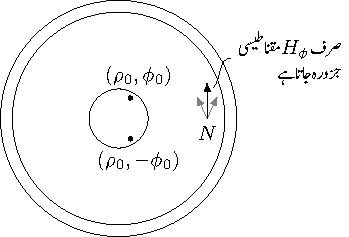
\includegraphics{figMagneticCoaxialRadialComponentsCancelOut}
\caption{رداسی اجزاء آپس میں ختم ہو جاتے ہیں اور یوں صرف زاویائی جزو رہ جاتا ہے۔}
\label{شکل_مقناطیسی_ہم_محوری_صرف_زاویائی_جزو}
\end{subfigure}%
\caption{ہم محوری تار۔}
\label{شکل_مقناطیسی_ہم_محوری_تار}
\end{figure}

ایمپیئر کے دوری قانون  کے استعمال کی دوسری مثال کی خاطر ہم شکل \حوالہ{شکل_مقناطیسی_ہم_محوری_تار} میں دکھائے گئے ہم محوری تار\فرہنگ{ہم محوری تار}\فرہنگ{coaxial} لیتے ہیں۔فرض کریں کہ \عددیء{z} محدد پر پڑی  ایسی لامحدود لمبائی کے ہم محوری  تار کے اندرونی حصے میں \عددیء{I} اور اس کے بیرونی سطح میں \عددیء{-I} برقی رو گزر رہی ہے۔اندرونی موصل موٹی ساخت کے تار کو نہایت پتلی فرضی تاروں کا مجموعہ تصور کیا جا سکتا ہے۔آئیں ان پتلی فرضی تاروں سے نقطہ \عددیء{N} پر پیدا مقناطیسی شدت پر غور کریں۔نقطہ \عددیء{N} کو کارتیسی محدد کے \عددیء{x} محدد پر رکھتے ہوئے مسئلے کی نوعیت شکل \حوالہ{شکل_مقناطیسی_ہم_محوری_تار}-ب میں دکھائی گئی ہے۔پچھلی مثال سے یہ واضح ہے کہ ایسی کسی بھی پتلی تار کی مقناطیسی شدت میں \عددیء{H_z} جزو نہیں پایا جاتا۔ساتھ ہی ساتھ ہم یہ بھی جانتے ہیں کہ ایسی تار کی مقناطیسی شدت تار کے گرد گول دائرہ بناتی ہے۔کسی بھی فرضی تار جو \عددیء{(\rho_0,\phi_0)} پر پائی جاتی ہو \عددیء{N} پر  \عددیء{\Delta H_{\rho}} اور \عددیء{\Delta H_{\phi}} اجزاء پیدا کرے گی۔اسی طرح \عددیء{(\rho_0,-\phi_0)} پر پتلی تار سے پیدا مقناطیسی شدت کے بھی ایسے رداسی اور زاویائی اجزاء ہوں گے۔ان دونوں پتلی تاروں کے رداسی اجزاء آپس میں الٹ سمت میں ہوں گے لہٰذا یہ ایک دوسرے کو ختم کریں گے جبکہ زاویائی اجزاء ایک ہی سمت میں ہوتے ہیں لہٰذا \عددیء{N} پر صرف زاویائی جزو پایا جائے گا۔

اندرونی ٹھوس موصل تار کے گرد ایسا گول دائرہ لیتے ہیں جس کا رداس \عددیء{\rho} اندرونی تار کے رداس \عددیء{\rho_1} سے زیادہ مگر بیرونی تار کے اندرونی رداس \عددیء{\rho_2} سے کم ہو۔اس راہ پر ہم ایمپیئر کے دوری قانون کی مدد سے
\begin{align}\label{مساوات_مقناطیسی_ہم_محوری_تاروں_کے_درمیان_شدت}
H_{\phi}=\frac{I}{2\pi \rho} \quad \quad (\rho_1 < \rho <\rho_2)
\end{align}
لکھ سکتے ہیں۔

اندرونی تار کا رقبہ عمودی تراش \عددیء{\pi \rho_1^2} ہے لہٰذا اس میں کثافت برقی رو \عددیء{\tfrac{I}{\pi \rho_1^2}} ہو گی۔اگر \عددیء{\rho} کو اندرونی ٹھوس موصل تار کے رداس \عددیء{\rho_1} سے کم رکھا جائے تب یہ راہ
\begin{align*}
I_{\textrm{گھیرا}}=\frac{I}{\pi \rho_1^2}\pi \rho^2=\frac{\rho^2}{\rho_1^2} I
\end{align*}
برقی رو کو گھیرے گا لہٰذا ایمپیئر کے دوری قانون کے تحت اندرونی ٹھوس تار میں
\begin{align*}
H_{\phi}=\frac{\rho I}{2\pi \rho_1^2} \quad \quad (\rho < \rho_1)
\end{align*}
مقناطیسی شدت پایا جائے گا۔اسی طرح اگر \عددیء{\rho} کو بیرونی تار کے بیرونی رداس \عددیء{\rho_3} سے زیادہ رکھا جائے تب یہ راہ اندرونی تار کے \عددیء{+I} اور بیرونی تار کے \عددیء{-I} کو گھیرے گی لہٰذا یہ  کل \عددیء{I-I=0} برقی رو کو گھیرے گا لہٰذا 
\begin{align*}
H_{\phi} =0 \quad \quad (\rho_3 < \rho)
\end{align*}
ہو گا۔آخر میں اس صورت کو بھی دیکھتے ہیں جب \عددیء{\rho} بیرونی تار کے اندر پایا جائے۔ایسی صورت میں یہ راہ
\begin{align*}
I_{\textrm{گھیرا}}=I-\left(\frac{\rho^2-\rho_2^2}{\rho_3^2-\rho_2^2}\right) I=\left(\frac{\rho_3^2-\rho^2}{\rho_3^2-\rho_2^2}\right)I
\end{align*}
برقی رو گھیرے گی لہٰذا بیرونی تار میں
\begin{align*}
H_{\phi}=\frac{I}{2\pi \rho} \left(\frac{\rho_3^2-\rho^2}{\rho_3^2-\rho_2^2} \right) \quad \quad (\rho_2<\rho<\rho_3)
\end{align*}
ہو گا۔ 

ہم محوری تار کے باہر مقناطیسی شدت صفر کے برابر ہے۔اس کی وجہ یہ ہے کہ تار کے باہر کوئی بھی بند گول دائرہ اندرونی تار کی برقی رو \عددیء{I} اور بیرونی تار کی برقی رو \عددیء{-I} دونوں کو گھیرتا ہے۔یہ دونوں برابر مقدار مگر الٹ سمت کے برقی رو ہر نقطے پر برابر مگر الٹ سمت میں مقناطیسی شدت پیدا کرتے ہیں جن کا مجموعہ صفر کے برابر ہوتا ہے۔ہم محوری تار کی یہ خاصیت کہ یہ بیرون تار کسی قسم کا مقناطیسی میدان نہیں پیدا کرتا انتہائی اہمیت کا حامل ہے۔ہم محوری تار اسی خاصیت کی بنا پر ہر ایسی جگہ پر استعمال کیا جاتا ہے جہاں تار میں پائے گئے برقی اشارات سے بیرونی تار کسی قسم کا اثر ناقابل برداشت ہو۔

ایمپیئر کے دوری قانون کے استعمال کی تیسری مثال کو شکل \حوالہ{شکل_مقناطیسی_لامحدود_سطحی_کثافت_برقی_رو}-الف میں دکھایا گیا ہے جہاں \عددیء{z=0} لامحدود چوڑائی اور لامحدود لمبائی کے موصل سطح پر \عددیء{K_x\ax} سطحی کثافت برقی رو گزر رہی ہے۔ہمیں اس سطح کے قریب نقطہ \عددیء{N} پر مقناطیسی شدت حاصل کرنے سے دلچسپی ہے۔سطح کے \عددیء{x=+\infty} سرے سے \عددیء{x=-\infty} سرے تک برقی رو بذریعہ دو لامحدود چوڑائی کے موصل سطحوں سے واپس پہنچتی ہے۔یہ سطحیں \عددیء{z=+\infty} اور \عددیء{z=-\infty} پر ہیں۔اتنی دور سطحوں کے اثر کو نقطہ \عددیء{N} پر نظر انداز کیا جا سکتا ہے۔

موصل سطح کو \عددیء{\Delta y} چوڑائی کی فرضی تاروں میں تقسیم کیا جا سکتا ہے۔ایسا شکل \حوالہ{شکل_مقناطیسی_لامحدود_سطحی_کثافت_برقی_رو}-ب میں دکھایا گیا ہے۔یوں ہر ایسی فرضی تار \عددیء{K_x \Delta y \ax} برقی رو گزارے گی۔لامحدود تار کے مقناطیسی میدان سے ہم بخوبی واقف ہیں۔ایسی کسی بھی فرضی تار کی برقی رو \عددیء{H_x} جزو پیدا نہیں کرے گا۔سطح پر \عددیء{N} کے ایک جانب فرضی تار کا \عددیء{H_z} جزو، سطح پر \عددیء{N} کے دوسری جانب فرضی تار کے \عددیء{H_z} جزو کو ختم کرتا ہے جبکہ ان  کے \عددیء{H_y} اجزاء مل کر دگنی مقناطیسی شدت پیدا کرتے ہیں۔اس طرح مقناطیسی شدت کا صرف اور صرف \عددیء{H_y} جزو ممکن ہے۔

\begin{figure}
\centering
\begin{subfigure}{0.5\textwidth}
\centering
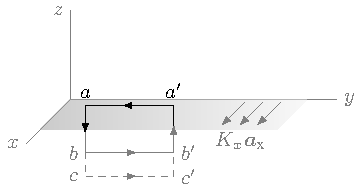
\includegraphics{figMagneticInfiniteSheetMagneticField}
\caption{لامحدود جسامت کے موصل سطح پر سطحی کثافت برقی رو۔}
\label{شکل_مقناطیسی_لامحدود_سطحی_برقی_رو}
\end{subfigure}%
%
\begin{subfigure}{0.5\textwidth}
\centering
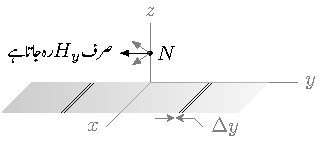
\includegraphics{figMagneticInfiniteSheetDividedIntoWires}
\caption{کسی بھی نقطے کے دونوں جانب فرضی تاروں کے \عددیء{H_z} اجزاء آپس میں ختم ہو جاتے ہیں جبکہ ان کے \عددیء{H_y} اجزاء جمع ہوتے ہیں۔}
\label{شکل_مقناطیسی_دونوں_جانب_زیڈ_اجزاء_ختم}
\end{subfigure}%
\caption{لامحدود سطحی کثافت برقی رو۔}
\label{شکل_مقناطیسی_لامحدود_سطحی_کثافت_برقی_رو}
\end{figure}
شکل \حوالہ{شکل_مقناطیسی_لامحدود_سطحی_کثافت_برقی_رو}-الف میں موصل سطح کے کچھ حصے کو گھیرتی ہوئی مستطیلی راہ \عددیء{a'abb'} دکھائی گئی ہے۔\عددی{aa'} یا \عددی{bb'} کی لمبائی \عددی{y_1} ہے جبکہ \عددی{ab} یا \عددی{a'b'} کی لمبائی \عددی{2z_1} ہے۔ اس راہ کے \عددیء{z_1} حصوں پر مقناطیسی شدت صفر کے برابر ہے لہٰذا اس حصے پر مقناطیسی شدت کا تکمل بھی صفر کے برابر ہو گا۔راہ کے \عددیء{y_1} اطراف سطح سے دونوں جانب \عددیء{z_1} فاصلے پر ہیں۔سطح کے دونوں اطراف بالکل یکساں مشابہت رکھتے ہیں۔بایوٹ-سیوارٹ کے قانون سے آپ دیکھ سکتے ہیں کہ سطحی کثافت برقی رو  موصل سطح کے اوپر جانب \عددیء{-H_{ya}\ay} جبکہ اس کے نچلی جانب  \عددیء{+H_{yb}\ay} مقناطیسی شدت پیدا کرتا ہے۔مستطیلی راہ \عددیء{Ky_1} برقی رو کو گھیرتی ہے لہٰذا ایمپیئر کے دوری قانون کے تحت
\begin{align*}
H_{ya} y_1+H_{yb} y_1=K_x y_1
\end{align*} 
یا
\begin{align}\label{مساوات_مقناطیسی_لامحدود_دونوں_اطراف}
H_{ya} +H_{yb}=K_x
\end{align} 
ہو گا۔اب اگر موصل سطح کے ایک جانب مستطیلی راہ کا \عددیء{y_1} حصہ قدر دور کرتے ہوئے \عددیء{z_2} فاصلے پر کر دیا جائے تب مندرجہ بالا مساوات 
\begin{align*}
H_{ya} +H_{yc}=K_x
\end{align*} 
صورت اختیار کر لے گی جس سے صاف ظاہر ہے کہ \عددیء{H_{yb}} اور \عددیء{H_{yc}} عین برابر ہیں یعنی مقناطیسی شدت کا دارومدار سطح سے فاصلے پر ہرگز نہیں ہے۔اس طرح تمام ایسے نقطے جو مثبت \عددیء{z} پر پائے جاتے ہوں پر مقناطیسی شدت برابر ہو گی۔یہی کچھ تمام ایسے نقطوں کے لئے بھی درست ہے جو منفی \عددیء{z} پر پائے جاتے ہوں۔ 

سطح کے دونوں اطراف بالکل یکساں مشابہت رکھتے ہیں لہٰذا دونوں جانب  مقناطیسی شدت بھی برابر ہو گا یعنی \عددیء{\abs{\kvec{H}_{ya}}=\abs{\kvec{H}_{yb}}} ہو گا۔اس طرح مساوات \حوالہ{مساوات_مقناطیسی_لامحدود_دونوں_اطراف} سے \عددیء{H_{ya}=H_{yb}=H_y=\tfrac{K_x}{2}} لکھتے ہوئے
\begin{align*}
\kvec{H}_{y}&=-\frac{1}{2}K_x \ax \quad \quad (z>0)\\
\kvec{H}_{y}&=+\frac{1}{2}K_x \ax \quad \quad (z<0)
\end{align*}
حاصل ہوتا ہے جسے  بہتر طور پر 
\begin{align}
\kvec{H}=\frac{1}{2} \kvec{K} \times \aN
\end{align}
لکھا جا سکتا ہے جہاں \عددیء{\aN} موصل سطح کی عمودی اکائی سمتیہ ہے۔

اگر \عددیء{z=-h} پر دوسری لامحدود موصل سطح رکھی جائے جس میں سطحی کثافت برقی رو \عددیء{-K_x\ax} ہو تب دونوں سطحی کثافت برقی رو کی مجموعی مقناطیسی شدت
\begin{gather}
\begin{aligned}
\kvec{H}&=\kvec{K} \times \aN \quad \quad (-h <z < 0)\\
\kvec{H}&=0 \quad \quad \quad \quad  (z<-h, \quad z>0) 
\end{aligned}
\end{gather}
ہو گی۔

ایمپیئر کے دوری قانون کے استعمال میں سب سے مشکل کام ایسی راہ تلاش کرنا ہے جس پر مقناطیسی میدان یا راہ کے عمودی ہو اور یا پھر اس کی قیمت مستقل ہو۔جہاں قبل از وقت ایسا جاننا ممکن نہ ہو وہاں بایوٹ-سیوارٹ کا قانون ہی قابل استعمال ہو گا۔ 

\begin{figure}
\centering
\begin{subfigure}{0.4\textwidth}
\centering
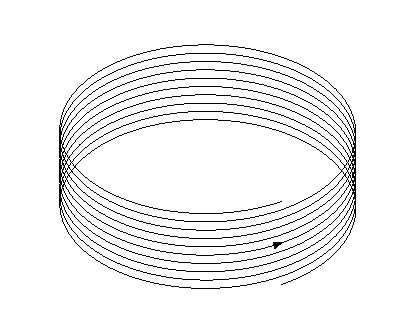
\includegraphics{figSteadyMagneticSolenoid}
\caption{پیچ دار لچھا۔}
\end{subfigure}%
%
\begin{subfigure}{0.4\textwidth}
\centering
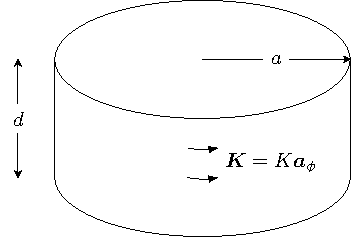
\includegraphics{figSteadyMagneticSolenoidAsSurfaceCurrent}
\caption{پیچدار لچھے کو سطحی کثافت تصور کیا جا سکتا ہے۔}
\end{subfigure}%
\caption{پیچدار لچھے کے میدان کا حصول۔}
\label{شکل-مقناطیسی_پیچدار_لچھا}
\end{figure}

آئیں ایمپیئر کے دوری قانون کو استعمال کرتے ہوئے شکل \حوالہ{شکل-مقناطیسی_پیچدار_لچھا}-الف میں دکھائے گئے، لا محدود لمبائی کے پیچدار لچھے\فرہنگ{پیچدار لچھا}\فرہنگ{لچھا!پیچدار}\فرہنگ{solenoid}\حاشیہب{solenoid}  کا مقناطیسی میدان حاصل کریں۔لچھے کا رداس \عددی{a} جبکہ اس میں لمبائی جانب  \عددی{d} فاصلے پر \عددی{N} چکر پائے جاتے ہیں جن میں برقی رو \عددی{I} گزر رہی ہے۔لچھے کا محور عین \عددی{z} محدد پر پایا جاتا ہے۔  

لچھے کے چکر انتہائی قریب قریب ہونے کی صورت میں لچھے  کے تاروں میں برقی رو کو سطحی کثافت رو تصور کیا جا سکتا ہے۔شکل  \حوالہ{شکل-مقناطیسی_پیچدار_لچھا}-ب میں ایسا ہی کرتے ہوئے لچھے کو نلکی سطحی کثافت 
\begin{align*}
\kvec{K}=K \aphi=\frac{NI}{d} \aphi
\end{align*}
تصور کیا گیا ہے۔سطحی کثافت برقی رو کی صورت میں سطح کے باہر مقناطیسی میدان صفر کے برابر ہو گا جبکہ اس کے اندر میدان نہ تو \عددی{\rho} اور نا ہی \عددی{\phi} پر منحصر ہے۔لامحدود لمبائی کی نلکی میں میدان \عددی{z} پر بھی منحصر نہیں ہو گا۔ساتھ ہی ساتھ میدان صرف اور صرف \عددی{\az} سمت میں ہو گا۔

نلکی کے اندر اور باہر، \عددی{z} محدد کے متوازی لمبائی \عددی{d} کے فرضی لکیروں کے سرے آپس میں جوڑنے سے بند راہ پر ایمپیئر کا دوری قانون لاگو کرتے ہوئے  میدان 
\begin{align}\label{مساوات_ساکن_میدان_پیچدار_لچھا}
\kvec{H}&=K \az=\frac{NI}{d}\az \quad \quad \textrm{\RL{نلکی کے اندر}}  \\
\kvec{H}&=0 \quad \quad\quad \quad\quad\quad \quad \textrm{\RL{نلکی کے باہر}}
\end{align}
حاصل ہوتا ہے۔

محدود لمبائی کی پیچدار لچھا جس کے چکر قریب قریب ہوں کا میدان مساوات \حوالہ{مساوات_ساکن_میدان_پیچدار_لچھا} ہی دیتی ہے۔یہ مساوات لچھے کے سروں اور تار سے دور میدان کی صحیح قیمت دیتی ہے۔


آئیں ایمپیئر کے دوری قانون کی ایک  اور مثال دیکھیں۔شکل \حوالہ{شکل-مقناطیسی_پیچدار_لچھا}-الف کے پیچدار لچھے کو دائری شکل دے کر شکل \حوالہ{شکل-مقناطیسی_اندرسہ}-الف حاصل ہوتا ہے۔  
\begin{figure}
\centering
\begin{subfigure}{0.4\textwidth}
\centering
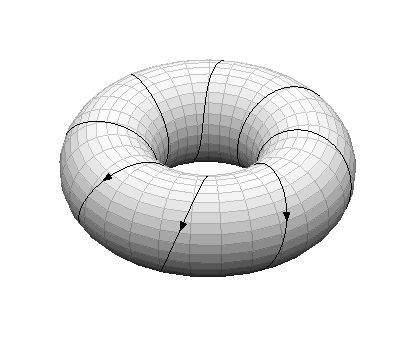
\includegraphics{figSteadyMagneticToroidalCoil}
\caption{اندرسہ لچھا۔}
\end{subfigure}%
%
\begin{subfigure}{0.4\textwidth}
\centering
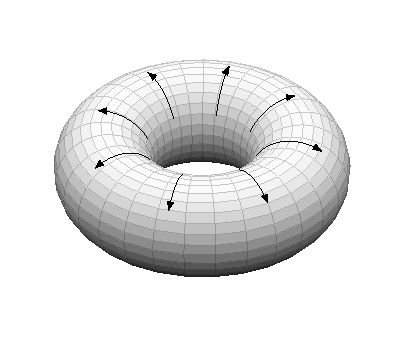
\includegraphics{figSteadyMagneticToroidCircularCrossSection}
\caption{اندرسہ کی سطح پر کثافت برقی رو پائی جاتی ہے۔}
\end{subfigure}%
\caption{اندرسہ کی سطح پر تار میں برقی رو کو کثافت برقی رو تصور کیا جا سکتا ہے۔}
\label{شکل-مقناطیسی_اندرسہ}
\end{figure}


شکل \حوالہ{شکل-مقناطیسی_اندرسہ}-الف میں اندرسہ\فرہنگ{اندرسہ}\فرہنگ{لچھا!اندرسہ}\حاشیہد{بچپن میں اندرسہ کس نے نہیں کھایا۔یہ شکل اندرسہ کی طرح ہے لہٰذا اس کتاب میں اسے اندرسہ ہی پکارا جائے گا۔اگر آپ کو مٹھائی پسند نہیں تو اسے سائیکل کے ٹائر میں موجود ٹیوب تصور کر سکتے ہیں۔}\حاشیہب{toroid}\فرہنگ{toroid} شکل کی سطح پر \عددی{N} چکر کی لپٹی تار میں \عددی{I} برقی رو گزر رہی ہے۔اندرسہ \عددی{z=0} سطح پر پڑی ہے جبکہ \عددی{z} محدد اس کے محور سے گزرتا ہے۔لپٹی تار کے چکر قریب قریب ہونے کی صورت میں اندرسے کی سطح پر \عددی{K} کثافت برقی رو تصور کی جا سکتی ہے۔اندرسے  کا عمودی تراش رداس \عددی{a} کا دائرہ ہے جبکہ اندرسے کا اوسط رداس \عددی{b} ہے۔اس طرح اندرسے  کا اندرونی رداس \عددی{b-a} جبکہ اس کا بیرونی رداس \عددی{b+a} ہو گا۔یوں اندرسے کے محور کے قریبی سطح پر کثافت برقی رو
\begin{align*}
K=\frac{NI}{2\pi (b-a)} \quad \si{\ampere\per\meter}
\end{align*}
ہو گی۔ایمپیئر کا دوری قانون استعمال کرنے کی غرض سے ہم اندرسے کے اندر رداس \عددی{(b-a)<\rho<(b+a)} کا دائرہ لیتے ہیں۔یہ فرضی دائرہ اندرسے کے محور کے قریبی سطح پر کثافت \عددی{K} کو گھیرے گا لہٰذا یہ 
\begin{align*}
2\pi (b-a) K
\end{align*}
برقی رو کو گھیرے گا۔یوں ایمپیئر کے دوری قانون سے اس رداس پر مقناطیسی میدان
\begin{gather}
\begin{aligned}
\kvec{H}&=\frac{2\pi (b-a) K}{2\pi \rho}=\frac{NI}{2\pi \rho} \aphi \quad \quad \textrm{\RL{اندرسے کے اندر}}  \\
\kvec{H}&=0  \quad \quad \quad \quad\quad \quad\quad \quad\quad \quad\textrm{\RL{اندرسے کے باہر}}
\end{aligned}
\end{gather}
ہو گا۔

شکل \حوالہ{شکل-مقناطیسی_اندرسہ}-الف میں تار کے چکر قریب قریب نہ ہونے کی صورت میں جب تک ہم دو چکر کے مابین فاصلے سے چند گنا زیادہ دور، تار سے ہٹ کر رہیں، یہی مساوات اصل میدان کی قیمت کے قریب قریب جواب دے گی۔
%====================
\حصہ{گردش}
آپ کو یاد ہو گا کہ ہم نے گاوس کے قانون کو انتہائی چھوٹی حجم پر لاگو کرتے ہوئے  \اصطلاح{پھیلاو} کی مساوات حاصل کی تھی۔اس حصے میں ہم ایمپیئر کے دوری قانون کو انتہائی چھوٹی بند راہ پر استعمال کرتے ہوئے \اصطلاح{گردش}\فرہنگ{گردش}\حاشیہب{curl}\فرہنگ{curl} کی مساوات حاصل کریں گے۔
\begin{figure}
\centering
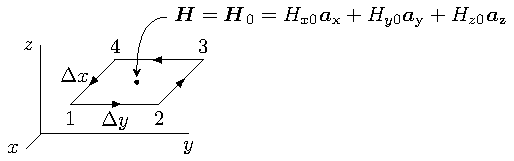
\includegraphics{figMagneticCurlDefined}
\caption{گردش کی تعریف۔ }
\label{شکل-مقناطیسی_گردش_تعریف}
\end{figure}

کارتیسی محدد میں ہم کسی نقطے \عددیء{N} پر  \عددیء{\Delta x} اور \عددیء{\Delta y} اطراف کی چھوٹی بند راہ لیتے ہیں۔شکل \حوالہ{شکل-مقناطیسی_گردش_تعریف} میں اس چھوٹی بند راہ کو دکھایا گیا ہے جو رقبہ \عددیء{\Delta x \Delta y} کو گھیرتی ہے۔یہ راہ مقناطیسی میدان \عددیء{{\kvec{H}=H_x\ax+H_y\ay+H_z\az}} میں پائی جاتی ہے۔شکل میں راہ پر تیر کے نشان راہ پر چلنے کی سمت کو ظاہر کرتے  ہیں۔اس رقبے کے عین وسط میں نقطہ \عددیء{(x_0,y_0,z_0)} پر مقناطیسی شدت 
\begin{align*}
\kvec{H}_0&=H_x(x_0,y_0,z_0)\ax+H_y(x_0,y_0,z_0)\ay+H_z(x_0,y_0,z_0)\az\\
&=H_{x0}\ax+H_{y0}\ay+H_{z0}\az
\end{align*}
کے برابر ہے۔ایمپیئر کے دوری قانون کے تحت اس بند راہ کے گرد مقناطیسی شدت کا تکمل رقبہ \عددیء{\Delta x \Delta y} سے گزرتی برقی رو کے برابر ہو گا۔آئیں اس تکمل کو حاصل کریں۔ایسا کرنے کی خاطر ہم بند راہ پر\عددیء{1} سے \عددیء{2} کی طرف چلتے ہوئے پورا چکر کاٹیں گے۔

کارتیسی محدد میں کسی بھی چھوٹے فاصلے کو \عددیء{\dif \kvec{L}=\dif x \ax+\dif y \ay+\dif z \az} لکھا جا سکتا ہے۔شکل \حوالہ{شکل-مقناطیسی_گردش_تعریف} میں \عددیء{1} تا \عددیء{2} پر \عددیء{\dif x=0} اور \عددیء{\dif z=0} ہیں لہٰذا اس چھوٹے فاصلے کو \عددیء{\dif \kvec{L}=\dif y \ay} لکھا جا سکتا ہے۔چھوٹے چکور کا وسط \عددیء{(x_0,y_0,z_0)} ہے۔یوں چکور کا \عددیء{1} کونا \عددیء{(x_0+\tfrac{\Delta x}{2},y_0-\tfrac{\Delta y}{2})} پر اور \عددیء{2} کونا \عددیء{(x_0+\tfrac{\Delta x}{2},y_0+\tfrac{\Delta y}{2})} پر ہو گا۔یوں راہ کے پہلے حصے \عددیء{1} تا \عددیء{2} پر لکیری تکمل
\begin{align*}
\int\limits_{y_0-\tfrac{\Delta y}{2}}^{y_0+\tfrac{\Delta y}{2}}\left(H_x \ax+H_y\ay+H_z\az \right) \cdot \dif y \ay=\int\limits_{y_0-\tfrac{\Delta y}{2}}^{y_0+\tfrac{\Delta y}{2}}H_y  \dif y =H_{y21}\int\limits_{y_0-\tfrac{\Delta y}{2}}^{y_0+\tfrac{\Delta y}{2}}  \dif y=H_{y21}\Delta y
\end{align*}
لکھا جا سکتا ہے جہاں \عددیء{1} تا \عددیء{2} پر مقناطیسی شدت کو \عددیء{H_y} کے بجائے \عددیء{H_{y21}} لکھتے ہوئے اور اس راہ پر مقناطیسی شدت میں تبدیلی کو نظر انداز کرتے ہوئے  تکمل کے باہر لے جایا گیا۔ہمیں اس طرح کے تکمل بار بار حاصل کرنے ہوں گے لہٰذا اس پورے عمل کو ہم
\begin{align}\label{مساوات_مقناطیسی_پہلے_حصہ_تکمل}
\left( \kvec{H} \cdot \dif \kvec{L}\right)_{21}=H_{y21} \Delta y 
\end{align}
لکھیں گے۔ہمیں رقبے کے عین وسط میں مقناطیسی شدت معلوم ہے البتہ راہ کے پہلے حصے پر ہمیں اس کے بارے میں معلومات فراہم نہیں ہے۔ایسی صورت میں ہمیں \اصطلاح{ٹیلر تسلسل}\فرہنگ{ٹیلر تسلسل}\حاشیہب{Taylor series}\فرہنگ{Taylor series} کو بروئے کار لانا ہو گا۔

ٹیلر تسلسل
\begin{align*}
f(x+\delta x)=f(x)+\frac{1}{1!}\frac{\partial f}{\partial x} \delta x + \frac{1}{2!}\frac{\partial^2 f}{\partial x^2} (\delta x)^2+\cdots
\end{align*}
سے آپ بخوبی واقف ہیں جہاں \عددیء{\tfrac{\partial f}{\partial x}} اور دیگر تفرق کو نقطہ \عددیء{x} پر حاصل کیا جاتا ہے۔اگر اس میں \عددیء{\delta x =\tfrac{\Delta x}{2}} پر کیا جائے تو اس کی نئی شکل
\begin{align*}
f(x+\tfrac{\Delta x}{2})=f(x)+\frac{1}{1!}\frac{\partial f}{\partial x} \frac{\Delta x}{2} + \frac{1}{2!}\frac{\partial^2 f}{\partial x^2} \left(\frac{\Delta x}{2}\right)^2+\cdots
\end{align*}
حاصل ہوتی ہے جسے ہم اب استعمال کرتے ہیں۔


اگر نقطہ \عددیء{(x_0,y_0,z_0)} پر تفاعل \عددیء{H_y} کی قیمت \عددیء{H_y(x_0,y_0,z_0)} ہو تب نقطہ \عددیء{(x_0+\tfrac{\Delta x}{2},y_0,z_0)} پر اس کی قیمت مسئلہ ٹیلر سے 
\begin{align*}
H_y(x_0+\tfrac{\Delta x}{2},y_0,z_0)&=H_y(x_0,y_0,z_0)+\frac{\partial H_y}{\partial x} \frac{\Delta x}{2}+\cdots\\
&=H_{y0}+\frac{\partial H_y}{\partial x} \frac{\Delta x}{2}+\cdots
\end{align*}
حاصل ہوتی ہے جہاں \عددیء{\tfrac{\partial H_y}{\partial x}} کو نقطہ \عددیء{(x_0,y_0,z_0)} پر حاصل کیا جاتا ہے۔راہ \عددیء{1} تا \عددیء{2} پر مقناطیسی شدت کی قیمت ٹیلر تسلسل کے پہلے دو اجزاء سے حاصل کرتے ہوئے
\begin{align}\label{مساوات_مقناطیسی_راہ_پہلے_حصے_پر_شدت}
H_{y21} \overset{.}{=}H_{y0}+\frac{\partial H_y}{\partial x} \frac{\Delta x}{2}
\end{align}
لکھ کر مساوات \حوالہ{مساوات_مقناطیسی_پہلے_حصہ_تکمل} کو
\begin{align}\label{مساوات_مقناطیسی_پہلے_حصہ_تکمل_الف}
\left( \kvec{H} \cdot \dif \kvec{L}\right)_{21}\overset{.}{=}\left(H_{y0}+\frac{\partial H_y}{\partial x} \frac{\Delta x}{2} \right)\Delta y 
\end{align}
لکھا جا سکتا ہے۔

مساوات \حوالہ{مساوات_مقناطیسی_راہ_پہلے_حصے_پر_شدت} کو یوں بھی حاصل کیا جا سکتا ہے۔چھوٹے رقبے کے وسط میں \عددیء{x} کے ساتھ \عددیء{H_y} میں تبدیل ہونے کی شرح \عددیء{\tfrac{\partial H_y}{\partial x}} ہے۔ یوں اگر \عددیء{x} میں \عددیء{\Delta x} تبدیلی پیدا ہو تب  \عددیء{H_y} میں تبدیلی تقریباً 
 \عددیء{\tfrac{\partial H_y}{\partial x}\Delta x} ہو گی اور یوں اس کی نئی قیمت تقریباً \عددیء{H_y+\tfrac{\partial H_y}{\partial x}\Delta x} ہو گی۔اسی طرح اگر \عددیء{x} میں \عددیء{\tfrac{\Delta x}{2}} تبدیلی پیدا ہو تب  \عددیء{H_y} میں تبدیلی تقریباً \عددیء{\tfrac{\partial H_y}{\partial x}\tfrac{\Delta x}{2}} ہو گی اور یوں اس کی نئی قیمت تقریباً \عددیء{H_y+\tfrac{\partial H_y}{\partial x}\tfrac{\Delta x}{2}} ہو گی۔اب رقبے کے وسط سے  \عددیء{+\tfrac{\Delta x}{2}} فاصلے پر  \عددیء{1} تا \عددیء{2} راہ کا درمیانہ نقطہ ہے لہٰذا یہاں
\begin{align}\label{مساوات_مقناطیسی_راہ_پہلے_حصے_پر_شدت_دوبارہ}
H_{y21}\overset{.}{=}H_{y0}+\frac{\partial H_y}{\partial x}\frac{\Delta x}{2}
\end{align}
ہو گا جو عین مساوات \حوالہ{مساوات_مقناطیسی_راہ_پہلے_حصے_پر_شدت} ہی  ہے۔

راہ کے اگلے حصے یعنی \عددیء{2} تا \عددیء{3} یہی کچھ کرتے ہوئے
\begin{align}\label{مساوات_مقناطیسی_پہلے_حصہ_تکمل_ب}
\left( \kvec{H} \cdot \dif \kvec{L}\right)_{32}=H_{x32}(-\Delta x) \overset{.}{=}-\left(H_{x0}+\frac{\partial H_x}{\partial y} \frac{\Delta y}{2} \right)\Delta x 
\end{align}
جبکہ \عددیء{3} تا \عددیء{4} پر
\begin{align}\label{مساوات_مقناطیسی_پہلے_حصہ_تکمل_پ}
\left( \kvec{H} \cdot \dif \kvec{L}\right)_{43}=H_{43}(-\Delta y)\overset{.}{=}-\left(H_{y0}-\frac{\partial H_y}{\partial x} \frac{\Delta x}{2} \right)\Delta y 
\end{align}
اور \عددیء{4} تا \عددیء{1} پر
\begin{align}\label{مساوات_مقناطیسی_پہلے_حصہ_تکمل_ت}
\left( \kvec{H} \cdot \dif \kvec{L}\right)_{14}=H_{x14}\Delta x \overset{.}{=}\left(H_{x0}-\frac{\partial H_x}{\partial y} \frac{\Delta y}{2} \right)\Delta x 
\end{align}
حاصل ہوتے ہیں۔مساوات  \حوالہ{مساوات_مقناطیسی_پہلے_حصہ_تکمل_الف}، مساوات \حوالہ{مساوات_مقناطیسی_پہلے_حصہ_تکمل_ب}، مساوات \حوالہ{مساوات_مقناطیسی_پہلے_حصہ_تکمل_پ} اور مساوات \حوالہ{مساوات_مقناطیسی_پہلے_حصہ_تکمل_ت} کو جمع کرتے ہوئے پورے بند راستے کا تکمل
\begin{align}
\oint \kvec{H} \cdot \dif \kvec{L}\overset{.}{=}\left(\frac{\partial H_y}{\partial x}-\frac{\partial H_x}{\partial y} \right)\Delta x \Delta y
\end{align}
حاصل ہوتا ہے۔اگر اس چھوٹے بند راہ کے گھیرے رقبے پر کثافت برقی رو
\begin{align*}
\kvec{J}=J_x \ax+J_y\ay+J_z \az
\end{align*}
ہو تب اس رقبے سے \عددیء{J_z \Delta x \Delta y} برقی رو گزرے گی۔ ایمپیئر کے دوری قانون کے تحت بند راہ کا تکمل اور رقبے سے گزرتی برقی رو برابر ہوں گے یعنی
\begin{align*}
\oint \kvec{H} \cdot \dif \kvec{L}\overset{.}{=}\left(\frac{\partial H_y}{\partial x}-\frac{\partial H_x}{\partial y} \right)\Delta x \Delta y\overset{.}{=}J_z \Delta x \Delta y
\end{align*}
ہو گا جسے
\begin{align*}
\frac{\oint \kvec{H} \cdot \dif \kvec{L}}{\Delta x \Delta y}\overset{.}{=}\frac{\partial H_y}{\partial x}-\frac{\partial H_x}{\partial y}\overset{.}{=}J_z
\end{align*}
لکھا جا سکتا ہے۔رقبے کو جتنا چھوٹا کیا جائے مندرجہ بالا مساوات اتنی ہی زیادہ درست ہو گی حتٰی کہ \عددیء{\Delta x \to 0} اور \عددیء{\Delta y \to 0} کی صورت میں یہ مکمل طور پر درست ہو گا اور یوں مساوات میں تقریباً برابر کی علامت \عددیء{\overset{.}{=}} کی جگہ بالکل برابر \عددیء{=} کی علامت استعمال کی جائے گی یعنی
\begin{align}\label{مساوات_مقناطیسی_گردش_الف}
\lim_{\overset{\Delta x \to 0}{\Delta y \to 0}}\frac{\oint \kvec{H} \cdot \dif \kvec{L}}{\Delta x \Delta y}=\frac{\partial H_y}{\partial x}-\frac{\partial H_x}{\partial y}=J_z
\end{align}
لکھا جائے گا۔

اگر ہم کارتیسی محدد کے بقایا دو محدد کے عمودی چھوٹے رقبے لیں اور مندرجہ بالا عمل دہرائیں تو ہمیں
\begin{align}\label{مساوات_مقناطیسی_گردش_ب}
\lim_{\overset{\Delta y \to 0}{\Delta z \to 0}}\frac{\oint \kvec{H} \cdot \dif \kvec{L}}{\Delta y \Delta z}=\frac{\partial H_z}{\partial y}-\frac{\partial H_y}{\partial z}=J_x
\end{align}
اور
\begin{align}\label{مساوات_مقناطیسی_گردش_پ}
\lim_{\overset{\Delta z \to 0}{\Delta x \to 0}}\frac{\oint \kvec{H} \cdot \dif \kvec{L}}{\Delta z \Delta x}=\frac{\partial H_x}{\partial z}-\frac{\partial H_z}{\partial x}=J_y
\end{align}
حاصل ہوں گے۔ مساوات \حوالہ{مساوات_مقناطیسی_گردش_ب} میں چھوٹے رقبے کے اطراف \عددیء{\Delta y} اور \عددیء{\Delta z} ہیں جس سے \عددیء{J_x \Delta y \Delta z} برقی رو گزرتی ہے۔اسی طرح مساوات \حوالہ{مساوات_مقناطیسی_گردش_پ} میں چھوٹے رقبے کے اطراف \عددیء{\Delta z} اور \عددیء{\Delta x} ہیں جس سے \عددیء{J_y \Delta z \Delta x} برقی رو گزرتی ہے۔

ایمپیئر کے دوری قانون سے شروع کرتے ہوئے ہم نے مساوات \حوالہ{مساوات_مقناطیسی_گردش_الف}، مساوات \حوالہ{مساوات_مقناطیسی_گردش_ب} اور مساوات \حوالہ{مساوات_مقناطیسی_گردش_پ} حاصل کئے جو مقناطیسی شدت کے بند تکمل فی اکائی رقبہ کو گھیرے گئے کثافت برقی رو کے برابر ٹہراتے ہیں۔کسی بھی متغیرہ کے بند تکمل فی اکائی رقبہ کو اس متغیرہ کی \اصطلاح{گردش}\فرہنگ{گردش}\حاشیہب{curl}\فرہنگ{curl} کہتے ہیں۔انتہائی چھوٹے رقبے کے گرد گردش کرتے ہوئے کسی بھی متغیرہ کے بند تکمل کو اس نقطے پر متغیرہ کے گھومنے یا  گردش کی ناپ تصور کی جا سکتی ہے۔اسی لئے اس عمل کو \اصطلاح{گردش} کہا جاتا ہے۔

کسی بھی سمتیہ کی گردش بھی سمتیہ ہو گی۔گردش کا کوئی بھی جزو انتہائی چھوٹے سیدھے رقبے کے گرد سمتیہ کے بند تکمل فی یہی رقبہ کے برابر ہو گا جہاں بند تکمل کی راہ درکار جزو کے عمودی سطح میں پایا جاتا ہو اور رقبے کی قیمت صفر کے قریب سے قریب تر ہو۔گردش کی یہ تعریف کسی بھی محدد پر مبنی نہیں ہے۔اس تعریف کی حسابی شکل
\begin{align*}
\kvec{H} \textrm{گردش}=\lim_{\Delta S_n \to 0} \frac{\oint \kvec{H} \cdot \dif \kvec{L}}{\Delta S_n}
\end{align*}
ہے جہاں \عددیء{\kvec{H}} کی گردش حاصل کی گئی ہے۔اس مساوات میں \عددیء{\Delta S_n} وہ چھوٹا سیدھا رقبہ ہے جس کے گرد \عددیء{\kvec{H}} کا بند تکمل حاصل کیا گیا ہے۔گردش از خود سیدھے  سطح کے عمودی ہو گا۔ رقبہ \عددیء{\Delta S_n} لکھتے ہوئے زیر نوشت میں \عددیء{n} اسی حقیقت کی یاد دہانی کراتا ہے کہ رقبے اور گردش کے درمیان نوے درجے کا زاویہ پایا جاتا ہے۔

کارتیسی محدد میں گردش \عددیء{\kvec{H}}  کے \عددیء{x}، \عددیء{y} اور \عددیء{z} اجزاء مساوات \حوالہ{مساوات_مقناطیسی_گردش_ب}، مساوات \حوالہ{مساوات_مقناطیسی_گردش_پ} اور مساوات \حوالہ{مساوات_مقناطیسی_گردش_الف} بالترتیب دیتے ہیں لہٰذا
\begin{align}\label{مساوات_مقناطیسی_کارتیسی_گردش_الف}
\kvec{H} \textrm{گردش}=\left(\frac{\partial H_z}{\partial y}-\frac{\partial H_y}{\partial z} \right)\ax+\left( \frac{\partial H_x}{\partial z}-\frac{\partial H_z}{\partial x}\right)\ay+\left(\frac{\partial H_y}{\partial x}-\frac{\partial H_x}{\partial y} \right)\az=\kvec{J}
\end{align}
لکھا جا سکتا ہے۔اس مساوات  کو قالب کے  \اصطلاح{حتمی قیمت}\فرہنگ{قالب!حتمی قیمت}\حاشیہب{determinant}\فرہنگ{determinant} کی شکل میں
\begin{align}
\kvec{H} \textrm{گردش}=
\begin{vmatrix}
\ax & \ay & \az\\
\frac{\partial }{\partial x}&\frac{\partial }{\partial y}&\frac{\partial }{\partial z}\\
H_x & H_y & H_z
\end{vmatrix}=\kvec{J}
\end{align}
لکھا جا سکتا ہے۔صفحہ \حوالہصفحہ{مساوات-گاوس_نیبلا} پر مساوات \حوالہ{مساوات-گاوس_نیبلا} نیبلا \عددیء{\nabla} کے عمل کو بیان کرتا ہے جسے یہاں دوبارہ پیش کرتے ہیں
\begin{align*}
\nabla= \frac{\partial}{\partial x}\ax+\frac{\partial}{\partial y} \ay+\frac{\partial}{\partial z}\az
\end{align*}

اور صفحہ \حوالہصفحہ{مساوات_سمتیات_سمتی_ضرب_قالب_شکل} پر مساوات \حوالہ{مساوات_سمتیات_سمتی_ضرب_قالب_شکل} دو سمتیات کا سمتی ضرب دیتا ہے۔ان  سے گردش نہایت خوبصورتی سے
\begin{align}
\kvec{H} \textrm{گردش}=\nabla \times \kvec{H}
\end{align}
لکھی جا سکتی ہے۔آپ جلد دیکھیں گے کہ صرف کارتیسی محدد میں ہی گردش \عددیء{\nabla} اور \عددیء{\kvec{H}} کے صلیبی ضرب سے حاصل ہوتا ہے۔اس کے باوجود کسی بھی محدد میں گردش کو \عددیء{\nabla \times \kvec{H}} سے ہی ظاہر کیا جاتا ہے۔یوں کارتیسی محدد میں \عددیء{H} کی گردش یوں لکھی جائے گی۔
\begin{align}\label{مساوات_مقناطیسی_کارتیسی_گردش_ب}
\nabla \times \kvec{H}=\left(\frac{\partial H_z}{\partial y}-\frac{\partial H_y}{\partial z} \right)\ax+\left( \frac{\partial H_x}{\partial z}-\frac{\partial H_z}{\partial x}\right)\ay+\left(\frac{\partial H_y}{\partial x}-\frac{\partial H_x}{\partial y} \right)\az
\end{align}

\اصطلاح{ایمپیئر کے دوری}\فرہنگ{ایمپیئر!دوری قانون نقطہ شکل} قانون کی نقطہ شکل
\begin{align}\label{مساوات-مقناطیسی_مقناطیسی_گردش_صفر}
\nabla \times \kvec{H}=\kvec{J}
\end{align}
لکھی جا سکتی ہے جو  میکس ویل\فرہنگ{میکس ویل مساوات}\فرہنگ{Maxwell equation} کی دوسری مساوات ہے جو وقت کے ساتھ تبدیل نہ ہوتے میدان کے لئے درست ہے۔یہاں میکس ویل کی تیسری مساوات کا بھی ذکر کر لیتے ہیں جو \عددیء{\oint \kvec{E} \cdot \dif \kvec{L}} کی نقطہ شکل
\begin{align}\label{مساوات-مقناطیسی_برقی_گردش_صفر}
\nabla \times \kvec{E}=0
\end{align}
ہے۔ میکس ویل کے چوتھی مساوات پر اس کتاب میں آگے غور کیا جائے گا۔

آپ جانتے ہیں کہ ساکن برقی میدان  بقائی میدان ہوتا ہے لہٰذا اس میں بار \عددیء{q} کو کسی بھی بند راہ پر پورا چکر گھمانے کے لئے صفر توانائی درکار ہو گی۔یوں \عددیء{q\oint \kvec{E} \cdot \dif \kvec{L}} صفر کے برابر ہو گا جس سے \عددیء{\kvec{E}} کا گردش بھی صفر ہو گا۔مساوات \حوالہ{مساوات-مقناطیسی_برقی_گردش_صفر} یہی کہتی ہے۔اس کے برعکس وقت کے ساتھ غیر تغیر پذیر مقناطیسی میدان غیر بقائی میدان ہے جس میں بار کو برقی رو گھیرتی ہوئی کسی بھی بند راہ پر پورا چکر گھمانے کے لئے توانائی درکار ہو گی۔اسی لئے اس کی گردش صفر نہیں ہو گی۔مساوات \حوالہ{مساوات-مقناطیسی_مقناطیسی_گردش_صفر} یہی کہتی ہے۔

%=================

\ابتدا{مشق}
گردش یعنی \عددیء{\nabla \times \kvec{H}} کو
\begin{align*}
\left(\frac{\partial }{\partial x}\ax+\frac{\partial }{\partial y}\ay+\frac{\partial }{\partial z}\az \right) \times \left(H_x \ax+H_y \ay+H_z \az \right)
\end{align*}
لکھ کر سمتی ضرب سے مساوات \حوالہ{مساوات_مقناطیسی_کارتیسی_گردش_الف} حاصل کریں۔
\انتہا{مشق}
%=================
\ابتدا{مشق}
اگر \عددیء{\kvec{H}=(x^2 y+2z)\ax+(xz-y)\ay+(e^x yz)\az} تب \عددیء{\nabla \times \kvec{H}} کیا ہو گا اور اس کی قیمت نقطہ \عددیء{(0,1,2)} پر کیا ہو گی۔

جوابات:\عددیء{\nabla \times \kvec{H}=(e^x z-x)\ax+(2-e^x yz)\ay+(z-x^2)\az} اور نقطے پر گردش کی قیمت \عددیء{2\ax+2\az} ہو گی۔
\انتہا{مشق}

%==================
\ابتدا{مثال}
سمتیہ \عددیء{\kvec{A}=A_x\ax+A_y\ay+A_z\az} کے گردش کی گردش یعنی \عددیء{\nabla \times \nabla \times \kvec{A}} حاصل کریں۔

حل:مساوات \حوالہ{مساوات_مقناطیسی_کارتیسی_گردش_ب} سے 
\begin{align}
\nabla \times \kvec{A}=\left(\frac{\partial A_z}{\partial y}-\frac{\partial A_y}{\partial z} \right)\ax+\left( \frac{\partial A_x}{\partial z}-\frac{\partial A_z}{\partial x}\right)\ay+\left(\frac{\partial A_y}{\partial x}-\frac{\partial A_x}{\partial y} \right)\az
\end{align}
لکھتے  ہیں۔مساوات \حوالہ{مساوات_مقناطیسی_کارتیسی_گردش_ب} دوبارہ استعمال کرتے ہوئے 
\begin{align*}
\nabla \times \nabla \times \kvec{A}&=\left[\frac{\partial}{\partial y}\left(\frac{\partial A_y}{\partial x}-\frac{\partial A_x}{\partial y} \right)-\frac{\partial}{\partial z}\left( \frac{\partial A_x}{\partial z}-\frac{\partial A_z}{\partial x}\right) \right]\ax\\
& \quad +\left[ \frac{\partial }{\partial z}\left(\frac{\partial A_z}{\partial y}-\frac{\partial A_y}{\partial z} \right)-\frac{\partial }{\partial x}\left(\frac{\partial A_y}{\partial x}-\frac{\partial A_x}{\partial y} \right)\right]\ay\\
&\quad +\left[\frac{\partial }{\partial x}\left( \frac{\partial A_x}{\partial z}-\frac{\partial A_z}{\partial x}\right)-\frac{\partial }{\partial y} \left(\frac{\partial A_z}{\partial y}-\frac{\partial A_y}{\partial z} \right)\right]\az
\end{align*}
تمام تفرق حاصل کرتے ہوئے
\begin{align*}
\nabla \times \nabla \times \kvec{A}&=\left[\frac{\partial^2 A_y}{\partial y\partial x}-\frac{\partial^2 A_x}{\partial y^2} -\frac{\partial^2 A_x}{\partial z^2}+\frac{\partial^2 A_z}{\partial z\partial x} \right]\ax\\
& \quad +\left[ \frac{\partial^2 A_z}{\partial z\partial y}-\frac{\partial^2 A_y}{\partial z^2}-\frac{\partial^2 A_y}{\partial x^2}+\frac{\partial^2 A_x}{\partial x\partial y} \right]\ay\\
&\quad +\left[ \frac{\partial^2 A_x}{\partial x\partial z}-\frac{\partial^2 A_z}{\partial x^2}- \frac{\partial^2 A_z}{\partial y^2}+\frac{\partial^2 A_y}{\partial y\partial z} \right]\az
\end{align*}
اس مساوات کے پہلے جزو میں \عددیء{\mp \tfrac{\partial^2 A_x}{\partial x^2}}، دوسرے جزو میں \عددیء{\mp \tfrac{\partial^2 A_y}{\partial y^2}} اور تیسرے میں \عددیء{\mp \tfrac{\partial^2 A_z}{\partial z^2}} شامل کرتے ہوئے ذرہ مختلف ترتیب سے لکھتے ہیں۔
\begin{gather}
\begin{aligned}\label{مساوات_مقناطیسی_گردش_کی_گردش_الف}
\nabla \times \nabla \times \kvec{A}&=\left[\frac{\partial^2 A_x}{\partial x^2}+\frac{\partial^2 A_y}{\partial y\partial x}+\frac{\partial^2 A_z}{\partial z\partial x}\right]\ax-\left[\frac{\partial^2 A_x}{\partial x^2}+\frac{\partial^2 A_x}{\partial y^2} +\frac{\partial^2 A_x}{\partial z^2} \right]\ax\\
& \quad +\left[\frac{\partial^2 A_x}{\partial x\partial y}+\frac{\partial^2 A_y}{\partial y^2}+ \frac{\partial^2 A_z}{\partial z\partial y}\right]\ay-\left[\frac{\partial^2 A_y}{\partial x^2}+\frac{\partial^2 A_y}{\partial y^2}+\frac{\partial^2 A_y}{\partial z^2} \right]\ay\\
&\quad +\left[ \frac{\partial^2 A_x}{\partial x\partial z}+\frac{\partial^2 A_y}{\partial y\partial z}+\frac{\partial^2 A_z}{\partial z^2}\right]\az-\left[\frac{\partial^2 A_z}{\partial x^2}+\frac{\partial^2 A_z}{\partial y^2}+ \frac{\partial^2 A_z}{\partial z^2} \right]\az
\end{aligned}
\end{gather}
یہاں رک کر \عددیء{\kvec{A}} کے پھیلاو کی ڈھلوان یعنی \عددیء{\nabla (\nabla \cdot \kvec{A})} حاصل کرتے ہیں۔پھیلاو
\begin{align*}
\nabla \cdot \kvec{A}=\frac{\partial A_x}{\partial x}+\frac{\partial A_y}{\partial y}+\frac{\partial A_z}{\partial z}
\end{align*}
استعمال کرتے ہوئے
\begin{gather}
\begin{aligned}
\nabla \left(\nabla \cdot \kvec{A} \right)&=\left(\frac{\partial^2 A_x}{\partial x^2}+\frac{\partial^2 A_y}{\partial x  \partial y}+\frac{\partial^2 A_z}{\partial x  \partial z} \right)\ax\\
&\quad +\left(\frac{\partial^2 A_x}{\partial y \partial x}+\frac{\partial^2 A_y}{\partial y^2}+\frac{\partial^2 A_z}{\partial y  \partial z} \right)\ay\\
&\quad +\left(\frac{\partial^2 A_x}{\partial z \partial x}+\frac{\partial^2 A_y}{\partial z\partial y}+\frac{\partial^2 A_z}{\partial z^2} \right)\az\\
\end{aligned}
\end{gather}
حاصل ہوتا ہے۔اگر ہم
\begin{gather}
\begin{aligned}\label{مساوات_مقناطیسی_سمتی_لاپلاسی}
\nabla^2 \kvec{A} &\equiv \nabla^2 A_x \ax+\nabla^2 A_y \ay+\nabla^2 A_z \az\\
&=\left(\frac{\partial^2 A_x}{\partial x^2}+\frac{\partial^2 A_x}{\partial y^2}+\frac{\partial^2 A_x}{\partial z^2} \right)\ax+\left(\frac{\partial^2 A_y}{\partial x^2}+\frac{\partial^2 A_y}{\partial y^2}+\frac{\partial^2 A_y}{\partial z^2} \right)\ay+\left(\frac{\partial^2 A_z}{\partial x^2}+\frac{\partial^2 A_z}{\partial y^2}+\frac{\partial^2 A_z}{\partial z^2} \right)\az
\end{aligned}
\end{gather}
لکھیں تب مندرجہ بالا دو مساواتوں کی مدد سے مساوات \حوالہ{مساوات_مقناطیسی_گردش_کی_گردش_الف} کو یوں لکھا جا سکتا ہے۔
\begin{align}\label{مساوات_مقناطیسی_گردش_کی_گردش_ب}
\nabla \times \nabla \times \kvec{A} \equiv \nabla \left(\nabla \cdot \kvec{A} \right)-\nabla^2 \kvec{A}
\end{align}
مساوات \حوالہ{مساوات_مقناطیسی_سمتی_لاپلاسی} سمتیہ کی \اصطلاح{لاپلاسی}\فرہنگ{لاپلاس!سمتی}\حاشیہب{vector Laplacian}\فرہنگ{Laplacian!vector} ہے۔
\انتہا{مثال}
%==================
\ابتدا{مثال}\شناخت{مثال_مقناطیسی_سمتیہ_ضرب_مقداری_کی_گردش}
سمتیہ \عددیء{\kvec{S}} اور مقداری \عددیء{M} کے حاصل ضرب کی گردش کے لئے ثابت کریں کہ
\begin{align}
\nabla \times \left(M\kvec{S}\right) \equiv \left(\nabla M\right) \times \kvec{S}+M \left(\nabla \times \kvec{S}\right)
\end{align}
کے برابر ہے۔

حل:سمتیہ اور مقداری کے حاصل ضرب کو
\begin{align*}
M \kvec{S}=M\left(S_x\ax+S_y\ay+S_z\az \right)=M S_x\ax+M S_y\ay+M S_z\az
\end{align*}
لکھتے ہوئے اس کی گردش مساوات \حوالہ{مساوات_مقناطیسی_کارتیسی_گردش_ب} کی طرح لکھ کر
\begin{align*}
\nabla \times M\kvec{S}&=\left(\frac{\partial MS_z}{\partial y}-\frac{\partial MS_y}{\partial z} \right)\ax+\left( \frac{\partial MS_x}{\partial z}-\frac{\partial MS_z}{\partial x}\right)\ay+\left(\frac{\partial MS_y}{\partial x}-\frac{\partial MS_x}{\partial y} \right)\az
\end{align*}
تفرق کھولتے ہیں۔
\begin{align*}
\nabla \times M\kvec{S}&=\left(\frac{\partial M}{\partial y}S_z+M\frac{\partial S_z}{\partial y}-\frac{\partial M}{\partial z}S_y-M\frac{\partial S_y}{\partial z} \right)\ax\\
&\quad +\left( \frac{\partial M}{\partial z}S_x+M\frac{\partial S_x}{\partial z}-\frac{\partial M}{\partial x}S_z-M\frac{\partial S_z}{\partial x}\right)\ay \\
&\quad +\left(\frac{\partial M}{\partial x}S_y+M\frac{\partial S_y}{\partial x}-\frac{\partial M}{\partial y}S_x-M\frac{\partial S_x}{\partial y} \right)\az
\end{align*}
اس کو یوں ترتیب دیتے ہیں
\begin{align*}
\nabla \times M\kvec{S}&=\left[\left(\frac{\partial M}{\partial y}S_z-\frac{\partial M}{\partial z}S_y\right)\ax+\left( \frac{\partial M}{\partial z}S_x-\frac{\partial M}{\partial x}S_z\right)\ay+\left(\frac{\partial M}{\partial x}S_y-\frac{\partial M}{\partial y}S_x\right)\az\right]\\
&\quad +M\left[\left(\frac{\partial S_z}{\partial y}-\frac{\partial S_y}{\partial z} \right)\ax+\left(\frac{\partial S_x}{\partial z}-\frac{\partial S_z}{\partial x}\right)\ay +\left(\frac{\partial S_y}{\partial x}-\frac{\partial S_x}{\partial y} \right)\az\right]
\end{align*}
اس مساوات کا دوسرا جزو \عددیء{M (\nabla \times \kvec{S})} کے برابر ہے جبکہ اس کا پہلا جزو \عددیء{(\nabla M)\times \kvec{S}} کے برابر ہے جسے 
\begin{align*}
\left(\nabla M\right) \times \kvec{S}=\left(\frac{\partial M}{\partial x}\ax+\frac{\partial M}{\partial y}\ay+\frac{\partial M}{\partial z}\az \right) \times \left(S_x \ax+S_y \ay +S_z \az \right)
\end{align*}
لکھ کر صلیبی ضرب کے بعد ترتیب دینے سے
\begin{align*}
\left(\nabla M\right) \times \kvec{S}=\left(\frac{\partial M}{\partial y}S_z-\frac{\partial M}{\partial z}S_y\right)\ax+\left( \frac{\partial M}{\partial z}S_x-\frac{\partial M}{\partial x}S_z\right)\ay+\left(\frac{\partial M}{\partial x}S_y-\frac{\partial M}{\partial y}S_x\right)\az
\end{align*}
حاصل کیا جا سکتا ہے۔
\انتہا{مثال}
%==================
\جزوحصہ{نلکی محدد میں گردش}
نلکی محدد میں \عددیء{J_z} کثافت برقی رو کے عمودی سطح پر چھوٹا رقبہ لیتے ہیں جسے شکل \حوالہ{شکل_مقناطیسی_نلکی_شدت_رقبہ} میں دکھایا گیا ہے۔ایسے رقبے کے اطراف \عددیء{\Delta \rho} اور \عددیء{\rho \Delta \phi} ہوں گے جبکہ اس سطح پر \عددیء{z} کی قیمت تبدیل نہیں ہو گی۔اس رقبے کے وسط میں
\begin{align*}
\kvec{H}_0(\rho_0,\phi_0,z_0)&=H_{\rho 0}\arho+H_{\phi 0}\aphi+H_{z 0}\az
\end{align*}
ہو گا۔کارتیسی محدد میں رقبے کے وسط سے \عددیء{+\tfrac{\Delta x}{2}} اور \عددیء{-\tfrac{\Delta x}{2}} فاصلے پر اطراف کی لمبائیاں عین برابر تھیں۔نلکی محدد میں رقبے کے وسط سے \عددیء{+\tfrac{\Delta \rho}{2}} فاصلے پر طرف کی لمبائی \عددیء{(\rho_0+\tfrac{\Delta \rho}{2})\Delta \phi} جبکہ  وسط سے \عددیء{-\tfrac{\Delta \rho}{2}} فاصلے پر طرف کی لمبائی \عددیء{(\rho_0-\tfrac{\Delta \rho}{2})\Delta \phi} ہے۔انہیں اطراف پر مقناطیسی شدت  بالترتیب
\begin{align*}
H_{\phi 21}\overset{.}{=}H_{\phi 0}+\frac{\partial H_\phi}{\partial \rho}\frac{\Delta \rho}{2}
\end{align*}
اور
\begin{align*}
H_{\phi 43}\overset{.}{=}H_{\phi 0}-\frac{\partial H_\phi}{\partial \rho}\frac{\Delta \rho}{2}
\end{align*}
ہو گی جہاں \عددیء{\tfrac{\partial H_\phi}{\partial \rho}} چھوٹے رقبے کے وسط میں حاصل کیا جائے گا۔یوں \عددیء{1} سے \عددیء{2} جانب چھوٹے رقبے کے گرد چکر کاٹتے ہوئے ان دو اطراف پر تکمل
\begin{align*}
(\kvec{H} \cdot \dif \kvec{L})_{21}&\overset{.}{=}\left(H_{\phi 0}+\frac{\partial H_\phi}{\partial \rho}\frac{\Delta \rho}{2} \right)\left(\rho_0 +\frac{\Delta \rho}{2} \right)\Delta \phi\\
&\overset{.}{=}\left[H_{\phi 0} \rho_0+H_{\phi 0} \frac{\Delta \rho}{2}+\rho_0 \frac{\partial H_\phi}{\partial \rho}\frac{\Delta \rho}{2}+\frac{\partial H_\phi}{\partial \rho} \left(\frac{\Delta \rho}{2} \right)^2\right]\Delta \phi
\end{align*}
اور
\begin{align*}
(\kvec{H} \cdot \dif \kvec{L})_{43}&\overset{.}{=}\left(H_{\phi 0}-\frac{\partial H_\phi}{\partial \rho}\frac{\Delta \rho}{2} \right)\left[-\left(\rho_0 -\frac{\Delta \rho}{2} \right)\Delta \phi\right]\\
&\overset{.}{=}\left[-H_{\phi 0} \rho_0+H_{\phi 0} \frac{\Delta \rho}{2}+\rho_0 \frac{\partial H_\phi}{\partial \rho}\frac{\Delta \rho}{2}-\frac{\partial H_\phi}{\partial \rho} \left(\frac{\Delta \rho}{2} \right)^2\right]\Delta \phi
\end{align*}
ہوں گے۔
\begin{figure}
\centering
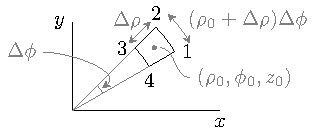
\includegraphics{figMagneticCurlCylindrical}
\caption{نلکی محدد میں چھوتا رقبہ۔}
\label{شکل_مقناطیسی_نلکی_شدت_رقبہ}
\end{figure}

چھوٹے رقبے کے وسط سے \عددیء{+\tfrac{\Delta \phi}{2}}  یا \عددیء{-\tfrac{\Delta \phi}{2}} پر  اطراف
 \عددیء{\Delta \rho} لمبائی رکھتے ہیں جبکہ ان پر اوسط شدت بالترتیب
\begin{align*}
H_{\phi 32}\overset{.}{=}H_{\rho 0}+\frac{\partial H_\rho}{\partial \phi}\frac{\Delta \phi}{2}
\end{align*}
اور
\begin{align*}
H_{\phi 14}\overset{.}{=}H_{\rho 0}-\frac{\partial H_\rho}{\partial \phi}\frac{\Delta \phi}{2}
\end{align*}
ہیں۔یوں ان اطراف پر تکمل
\begin{align*}
\left(\kvec{H} \cdot \dif \kvec{L}\right)_{32} \overset{.}{=}\left(H_{\rho 0}+\frac{\partial H_\rho}{\partial \phi}\frac{\Delta \phi}{2} \right)\left(-\Delta \rho \right)
\end{align*}
اور
\begin{align*}
\left(\kvec{H} \cdot \dif \kvec{L}\right)_{14} \overset{.}{=}\left(H_{\rho 0}-\frac{\partial H_\rho}{\partial \phi}\frac{\Delta \phi}{2} \right)\Delta \rho
\end{align*}
ہوں گے۔

یوں پورا تکمل ان چار جوابات کا مجموعہ
\begin{align}\label{مساوات_مقناطیسی_نلکی_پہلا_بند_تکمل}
\oint\kvec{H} \cdot \dif \kvec{L}\overset{.}{=}\left(H_{\phi 0} +\rho_0 \frac{\partial H_\phi}{\partial \rho}-\frac{\partial H_\rho}{\partial \phi}\right)\Delta \rho \Delta \phi
\end{align}
ہو گا۔اس چھوٹے رقبے سے \عددیء{J_z \rho_0 \Delta \rho \Delta \phi} برقی رو گزرے گی۔یوں ایمپیئر کے دوری قانون سے
\begin{align*}
\oint \kvec{H} \cdot \dif \kvec{L}\overset{.}{=}\left(H_{\phi 0} +\rho_0 \frac{\partial H_\phi}{\partial \rho}-\frac{\partial H_\rho}{\partial \phi}\right)\Delta \rho \Delta \phi\overset{.}{=}J_z \rho_0 \Delta \rho \Delta \phi
\end{align*}
یعنی
\begin{align*}
\frac{\oint \kvec{H} \cdot \dif \kvec{L}}{\rho_0 \Delta \rho \Delta \phi}\overset{.}{=}\left(\frac{H_{\phi 0}}{\rho_0} +\frac{\partial H_\phi}{\partial \rho}-\frac{1}{\rho_0}\frac{\partial H_\rho}{\partial \phi}\right)\overset{.}{=}J_z
\end{align*}
لکھا جا سکتا ہے۔اگر \عددیء{\Delta \rho} اور \عددیء{\Delta \phi} کو کم سے کم کرتے ہوئے صفر کے قریب تر کر دیا جائے تب مندرجہ بالا مساوات بالکل درست ہو گی اور تقریباً برابر کی علامت \عددیء{\overset{.}{=}} کی جگہ برابر کی علامت \عددیء{=} استعمال کی جائے گی۔اس طرح گردش کا پہلا جزو 
\begin{align}\label{مساوات_مقناطیسی_رداسی_زیڈ_گردش}
\lim_{\overset{\Delta \rho \to 0}{\Delta \phi \to 0}}\frac{\oint \kvec{H} \cdot \dif \kvec{L}}{\rho_0 \Delta \rho \Delta \phi}=\left(\frac{H_{\phi 0}}{\rho_0} +\frac{\partial H_\phi}{\partial \rho}-\frac{1}{\rho_0}\frac{\partial H_\rho}{\partial \phi}\right)=J_z
\end{align}
لکھا جا سکتا ہے۔

\begin{figure}
\centering
\begin{subfigure}{0.5\textwidth}
\centering
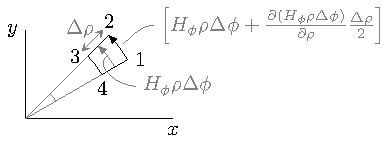
\includegraphics{figMagneticCurlCylindricalBetterRadialOut}
\caption{چھوٹے رقبے کے وسط پر تکمل کے قیمت سے بیرونی زاویائی تکمل کی قیمت کا حصول۔}
\end{subfigure}%
%
\begin{subfigure}{0.5\textwidth}
\centering
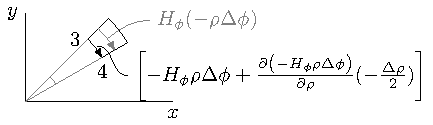
\includegraphics{figMagneticCurlCylindricalBetterRadialIn}
\caption{چھوٹے رقبے کے وسط پر تکمل کے قیمت سے اندرونی زاویائی تکمل کی قیمت کا حصول۔}
\end{subfigure}%
\caption{زاویائی حصوں پر تکمل کے قیمت کے حصول کا بہتر طریقہ۔}
\label{شکل_مقناطیسی_بہتر_گردش_نلکی}
\end{figure}
اس سے پہلے کہ ہم گردش کے بقایا دو اجزاء بھی حاصل کریں، آئیں مساوات \حوالہ{مساوات_مقناطیسی_نلکی_پہلا_بند_تکمل} کو قدر مختلف اور بہتر طریقے سے حاصل کریں۔شکل \حوالہ{شکل_مقناطیسی_بہتر_گردش_نلکی}-الف کو دیکھتے ہوئے آگے پڑھیں۔اگر ہم کسی نقطے  کے  \عددیء{-\tfrac{\Delta \phi}{2}} سے نقطے کے \عددیء{+\tfrac{\Delta \phi}{2}} تک حرکت کریں تو ہم \عددیء{\rho \Delta \phi}  فاصلہ طے کریں گے۔اس راہ پر تکمل تقریباً
\begin{align*}
\kvec{H} \cdot \dif \kvec{L}=H_{\phi}\rho \Delta \phi
\end{align*}
 کے برابر ہو گا۔اس تکمل کو تفاعل \عددیء{g} تصور کرتے ہوئے  یعنی \عددیء{g=H_{\phi}\rho \Delta \phi} لیتے ہوئے  ہم دیکھتے ہیں کہ اگر ہم چھوٹے رقبے کے وسط سے رداسی سمت میں  \عددیء{+\tfrac{\Delta \rho}{2}} حرکت کریں تو اس تفاعل کی قیمت میں تبدیلی
\begin{align*}
\Delta (\kvec{H} \cdot \dif \kvec{L})=\frac{\partial g}{\partial \rho}\frac{\Delta \rho}{2}=\frac{\partial (H_{\phi}\rho \Delta \phi)}{\partial \rho} \frac{\Delta \rho}{2}
\end{align*}
لکھی جا سکتی ہے جہاں \عددیء{\tfrac{\partial (H_{\phi}\rho \Delta \phi)}{\partial \rho}} کو چھوٹے رقبے کے وسط پر حاصل کیا جاتا ہے جہاں رداس \عددیء{\rho_0} کے برابر ہے۔چونکہ چھوٹے رقبے کے عین وسط پر اس تکمل کی قیمت \عددیء{H_{\phi 0}\rho_0 \Delta \phi} کے برابر ہے لہٰذا وسط سے \عددیء{\tfrac{\Delta \rho}{2}} فاصلے پر تکمل کی قیمت
\begin{align}\label{مساوات_مقناطیسی_نلکی_ایک_دو}
\kvec{H} \cdot \dif \kvec{L}_{21}=H_{\phi}\rho \Delta \phi+\frac{\partial (H_{\phi}\rho \Delta \phi)}{\partial \rho} \frac{\Delta \rho}{2}
\end{align}
ہو گی۔اسی طرح، جیسا شکل \حوالہ{شکل_مقناطیسی_بہتر_گردش_نلکی}-ب میں دکھایا گیا ہے، اگر ہم کسی نقطے کے  \عددیء{+\tfrac{\Delta \phi}{2}} سے نقطے کے  \عددیء{-\tfrac{\Delta \phi}{2}} تک حرکت کریں تو اس راہ پر تکمل
\begin{align*}
\kvec{H} \cdot \dif \kvec{L}=H_{\phi} (-\rho \Delta \phi)
\end{align*}
کے برابر ہو گا۔اگر اس نقطے کو چھوٹے رقبے کا وسط تصور کیا جائے تب وسط سے  \عددیء{-\tfrac{\Delta \rho}{2}} فاصلے پر یہی تکمل
\begin{gather}
\begin{aligned}\label{مساوات_مقناطیسی_نلکی_تین_چار}
\kvec{H} \cdot \dif \kvec{L}_{43}&=-H_{\phi}\rho \Delta \phi+\frac{\partial (-H_{\phi}\rho \Delta \phi)}{\partial \rho} \left(-\frac{\Delta \rho}{2}\right)\\
&=-H_{\phi}\rho \Delta \phi+\frac{\partial (H_{\phi}\rho \Delta \phi)}{\partial \rho} \frac{\Delta \rho}{2}
\end{aligned}
\end{gather}
ہو گا۔

اسی طرح، جیسے شکل \حوالہ{شکل_مقناطیسی_بہتر_گردش_نلکی_رداسی}-الف میں دکھایا گیا ہے، کسی بھی نقطے پر \عددیء{-\tfrac{\Delta \rho}{2}} تا \عددیء{+\tfrac{\Delta \rho}{2}} حرکت کرتے ہوئے تکمل کی قیمت \عددیء{H_{\rho} \Delta \rho} ہو گی۔اس نقطے سے \عددیء{-\tfrac{\Delta \phi}{2}} پر تکمل کی قیمت میں تبدیلی رو نما ہو گی جسے
\begin{align*}
\Delta  (\kvec{H} \cdot \dif \kvec{L})=\frac{\partial (H_{\rho} \Delta \rho)}{\partial \phi}\left(-\frac{\Delta \phi}{2}\right)
\end{align*}
لکھا جا سکتا ہے اور یوں تکمل کی نئی قیمت
\begin{align*}
\kvec{H} \cdot \dif \kvec{L}=H_{\rho} \Delta \rho-\frac{\partial (H_{\rho} \Delta \rho)}{\partial \phi}\frac{\Delta \phi}{2}
\end{align*}
ہو گی۔اگر چھوٹے رقبے کے عین وسط کو یہی نقطہ تصور کیا جائے تب مندرجہ بالا مساوات \عددیء{4} تا \عددیء{1} پر تکمل دیتا ہے یعنی
\begin{align}\label{مساوات_مقناطیسی_نلکی_چار_ایک}
\kvec{H} \cdot \dif \kvec{L}_{14}=H_{\rho} \Delta \rho-\frac{\partial (H_{\rho} \Delta \rho)}{\partial \phi}\frac{\Delta \phi}{2}
\end{align}

\begin{figure}
\centering
\begin{subfigure}{0.5\textwidth}
\centering
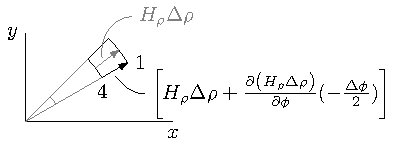
\includegraphics{figMagneticCurlCylindricalBetterAngularLess}
\caption{چھوٹے رقبے کے وسط پر رداسی تکمل کے قیمت سے کم زاویہ پر تکمل کی قیمت کا حصول۔}
\end{subfigure}%
%
\begin{subfigure}{0.5\textwidth}
\centering
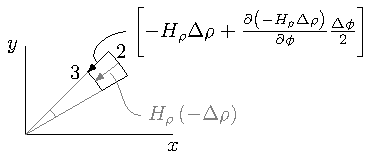
\includegraphics{figMagneticCurlCylindricalBetterAngularMore}
\caption{چھوٹے رقبے کے وسط پر رداسی تکمل کے قیمت سے زیادہ زاویہ پر تکمل کی قیمت کا حصول۔}
\end{subfigure}%
\caption{رداسی حصوں پر تکمل کے قیمت کے حصول کا بہتر طریقہ۔}
\label{شکل_مقناطیسی_بہتر_گردش_نلکی_رداسی}
\end{figure}
اسی طرح، جیسے شکل \حوالہ{شکل_مقناطیسی_بہتر_گردش_نلکی_رداسی}-ب میں دکھایا گیا ہے، کسی بھی نقطے پر \عددیء{+\tfrac{\Delta \rho}{2}} تا \عددیء{-\tfrac{\Delta \rho}{2}} حرکت کرتے ہوئے تکمل کی قیمت
\begin{align*}
\kvec{H} \cdot \dif \kvec{L}=H_{\rho}(-\Delta \rho)
\end{align*}
ہو گی۔اس نقطے کو چھوٹے رقبے کا وسط تصور کرتے ہوئے وسط  سے \عددیء{+\tfrac{\Delta \phi}{2}} پر یہی تکمل
\begin{align}\label{مساوات_مقناطیسی_نلکی_دو_تین}
\kvec{H} \cdot \dif \kvec{L}_{32}=-H_{\rho} \Delta \rho-\frac{\partial (H_{\rho} \Delta \rho)}{\partial \phi}\frac{\Delta \phi}{2}
\end{align}
کے برابر ہو گا۔

مساوات \حوالہ{مساوات_مقناطیسی_نلکی_ایک_دو}، مساوات \حوالہ{مساوات_مقناطیسی_نلکی_تین_چار}، مساوات \حوالہ{مساوات_مقناطیسی_نلکی_چار_ایک} اور مساوات \حوالہ{مساوات_مقناطیسی_نلکی_دو_تین} کا مجموعہ چھوٹے رقبے کے گرد پورا تکمل دیتا ہے یعنی
\begin{gather}
\begin{aligned}\label{مساوات_مقناطیسی_نلکی_پہلا_بند_تکمل_دوبارہ}
\oint \kvec{H} \cdot \dif \kvec{L}&=\frac{\partial (H_{\phi}\rho \Delta \phi)}{\partial \rho}\Delta \rho-\frac{\partial (H_{\rho} \Delta \rho)}{\partial \phi}\Delta \phi\\
&=\left[\frac{\partial (H_{\phi}\rho )}{\partial \rho}-\frac{\partial H_{\rho}}{\partial \phi}\right] \Delta \rho\Delta \phi
\end{aligned}
\end{gather}
جہاں تفرق رقبے کے وسط پر حاصل کئے جاتے ہیں۔اس مساوات کو یوں بھی لکھا جا سکتا ہے
\begin{align*}
\oint \kvec{H} \cdot \dif \kvec{L}&=\left[H_{\phi 0} +\rho_0 \frac{\partial H_{\phi}}{\partial \rho}-\frac{\partial H_{\rho}}{\partial \phi}\right] \Delta \rho\Delta \phi
\end{align*}
جو بالکل مساوات \حوالہ{مساوات_مقناطیسی_نلکی_پہلا_بند_تکمل} ہی ہے۔یاد رہے کہ \عددیء{\tfrac{\partial (H_{\phi}\rho)}{\partial \rho}} کو چھوٹے رقبے کے وسط میں حاصل کیا جائے گا۔یوں رداس \عددیء{\rho_0}  اور مقناطیسی شدت \عددیء{H_{\phi 0}} کے برابر ہوں گے۔مساوات \حوالہ{مساوات_مقناطیسی_نلکی_پہلا_بند_تکمل_دوبارہ} سے گردش
\begin{align}\label{مساوات_مقناطیسی_رداسی_ذ_گردش}
\lim_{\overset{\Delta \rho \to 0}{\Delta \phi \to 0}} \frac{\oint \kvec{H} \cdot \dif \kvec{L}}{\Delta \rho \rho \Delta \phi}=\left[\frac{1}{\rho}\frac{\partial (H_{\phi}\rho )}{\partial \rho}-\frac{1}{\rho}\frac{\partial H_{\rho}}{\partial \phi}\right] =J_z
\end{align}

\begin{figure}
\centering
\begin{subfigure}{0.5\textwidth}
\centering
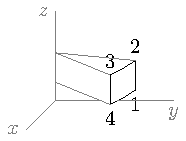
\includegraphics{figMagneticCurlCylindricalBetterRadialCurrentDensity}
\caption{نلکی محدد میں شدت کا رداسی جزو حاصل کرنے کے لئے چھوٹا رقبہ۔}
\end{subfigure}%
%
\begin{subfigure}{0.5\textwidth}
\centering
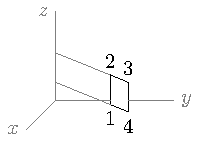
\includegraphics{figMagneticCurlCylindricalBetterAngularCurrentDensity}
\caption{نلکی محدد میں شدت کا زاویائی جزو حاصل کرنے کے لئے چھوٹا رقبہ۔}
\end{subfigure}%
\caption{نلکی محدد میں گردش کے رداسی اور زاویائی اجزاء کے رقبے۔}
\label{شکل_مقناطیسی_نلکی_رداسی}
\end{figure}

آئیں اب نلکی محدد میں گردش کے بقایا دو اجزاء بھی حاصل کریں۔گردش کا رداسی جزو حاصل کرنے کی خاطر ہم \عددیء{\rho=\rho_0} سطح پر چھوٹا رقبہ لیتے ہیں جس کے اطراف \عددیء{\Delta z} اور \عددیء{\rho_0 \Delta \phi} لمبائی رکھیں گے۔اس رقبے کو شکل \حوالہ{شکل_مقناطیسی_نلکی_رداسی}-الف میں دکھایا گیا ہے۔اس پر \عددیء{1} سے \عددیء{2} جانب گھومتے ہوئے \عددیء{} کا لکیری تکمل حاصل کیا جائے گا۔مستقل رداس کے سطح پر کسی بھی نقطے کے قریب \عددیء{-\tfrac{\Delta z}{2}} تا \عددیء{+\tfrac{\Delta z}{2}} چلتے ہوئے تکمل \عددیء{H_z \Delta z} حاصل ہوتا ہے۔اس نقطے سے  \عددیء{+\tfrac{\Delta \phi}{2}} زاویہ پر اس تکمل کی قیمت ٹیلر تسلسل سے
\begin{align*}
\kvec{H} \cdot \dif \kvec{L}_{21}=H_z \Delta z+\frac{\partial (H_z \Delta z)}{\partial \phi}\left(+\frac{\Delta \phi}{2}\right)
\end{align*}
حاصل ہوتی ہے۔اسی طرح نقطے  کے قریب \عددیء{+\tfrac{\Delta z}{2}} تا \عددیء{-\tfrac{\Delta z}{2}} چلتے ہوئے تکمل \عددیء{-H_z \Delta z} جبکہ نقطے سے \عددیء{-\tfrac{\Delta \phi}{2}} زاویہ پر
\begin{align*}
\kvec{H} \cdot \dif \kvec{L}_{43}=-H_z \Delta z+\frac{\partial (-H_z \Delta z)}{\partial \phi}\left(-\frac{\Delta \phi}{2}\right)
\end{align*}
حاصل ہوتا ہے۔ان دو جوابات سے رقبے کے \عددیء{z} اطراف کا تکمل
\begin{align}\label{مساوات_مقناطیسی_نلکی_رداسی_گردش_تکمل_الف}
\kvec{H} \cdot \dif \kvec{L}_{21}+\kvec{H} \cdot \dif \kvec{L}_{43}=+\frac{\partial H_z}{\partial \phi} \Delta z \Delta \phi
\end{align}
حاصل ہوتا ہے۔کسی بھی نقطے کے قریب \عددیء{-\tfrac{\Delta \phi}{2}} تا \عددیء{+\tfrac{\Delta \phi}{2}} پر تکمل کی قیمت \عددیء{H_{\phi}\rho \Delta \phi} جبکہ نقطے سے \عددیء{-\tfrac{\Delta z}{2}} فاصلے پر یہی تکمل ٹیلر تسلسل سے
\begin{align*}
\kvec{H} \cdot \dif \kvec{L}_{14}=H_{\phi} \rho \Delta \phi+\frac{\partial (H_{\phi} \rho \Delta \phi)}{\partial z}\left(-\frac{\Delta z}{2}\right)
\end{align*}
حاصل ہوتا ہے۔اسی طرح نقطے کے قریب \عددیء{+\tfrac{\Delta \phi}{2}} تا \عددیء{-\tfrac{\Delta \phi}{2}} پر تکمل کی
 قیمت \عددیء{-H_{\phi}\rho \Delta \phi} جبکہ نقطے سے \عددیء{+\tfrac{\Delta z}{2}} فاصلے پر یہی تکمل ٹیلر تسلسل سے
\begin{align*}
\kvec{H} \cdot \dif \kvec{L}_{32}=-H_{\phi} \rho \Delta \phi+\frac{\partial (-H_{\phi} \rho \Delta \phi)}{\partial z}\left(+\frac{\Delta z}{2}\right)
\end{align*}
حاصل ہوتا ہے۔ان دو جوابات کے مجموعے سے چھوٹے رقبے کے گرد گھومتے ہوئے زاویائی حصے کا تکمل
\begin{align}\label{مساوات_مقناطیسی_نلکی_رداسی_گردش_تکمل_ب}
 \kvec{H} \cdot \dif \kvec{L}_{14}+\kvec{H} \cdot \dif \kvec{L}_{32}=-\rho\frac{\partial H_{\phi} }{\partial z}\Delta z\Delta \phi
\end{align}
حاصل ہوتا ہے۔

مساوات \حوالہ{مساوات_مقناطیسی_نلکی_رداسی_گردش_تکمل_الف} اور مساوات \حوالہ{مساوات_مقناطیسی_نلکی_رداسی_گردش_تکمل_ب} کا مجموعہ چھوٹے رقبے کے گرد کل تکمل دیتا ہے جو رقبے سے گزرتی برقی رو \عددیء{J_{\rho}\rho \Delta \phi \Delta z} کے برابر ہو گا یعنی
\begin{align*}
\oint \kvec{H} \cdot \dif \kvec{L}=\left[ \frac{\partial H_z}{\partial \phi}-\rho\frac{\partial H_{\phi}}{\partial z} \right]\Delta z\Delta \phi=J_{\rho} \rho \Delta \phi \Delta z
\end{align*}
جس سے گردش کا رداسی جزو
\begin{align}\label{مساوات_مقناطیسی_رداسی_نلکی_گردش}
\lim_{\overset{\Delta \phi \to 0}{\Delta z \to 0}}\frac{\oint \kvec{H} \cdot \dif \kvec{L}}{\rho \Delta \phi \Delta z}=\left[\frac{1}{\rho}\frac{\partial H_z}{\partial \phi} -\frac{\partial H_{\phi}}{\partial z}\right]=J_{\rho}
\end{align}
ملتا ہے۔

شکل \حوالہ{شکل_مقناطیسی_نلکی_رداسی}-ب میں \عددیء{1} سے \عددیء{2} جانب گھومتے ہوئے  \عددیء{\kvec{H}} کے لکیری تکمل مندرجہ ذیل ہیں
\begin{align*}
\kvec{H} \cdot \dif \kvec{L}_{21}&=H_z \Delta z+\frac{\partial (H_z \Delta z)}{\partial \rho}\left(-\frac{\Delta \rho}{2}\right)\\
\kvec{H} \cdot \dif \kvec{L}_{43}&=-H_z \Delta z+\frac{\partial (-H_z \Delta z)}{\partial \rho}\left(+\frac{\Delta \rho}{2}\right)\\
\kvec{H} \cdot \dif \kvec{L}_{32}&=H_{\rho}\Delta \rho+\frac{\partial (H_{\rho}\Delta \rho)}{\partial  z}\frac{\Delta z}{2}\\
\kvec{H} \cdot \dif \kvec{L}_{14}&=-H_{\rho}\Delta \rho+\frac{\partial (-H_{\rho}\Delta \rho)}{\partial z}\left(-\frac{\Delta z}{2}\right)
\end{align*}
اور یوں ایمپیئر کے دوری قانون سے
\begin{align}\label{مساوات_مقناطیسی_زاویائی_نلکی_گردش}
\lim_{\overset{\Delta \rho \to 0}{\Delta z \to 0}}\frac{\oint \kvec{H} \cdot \dif \kvec{L}}{\Delta \rho \Delta z}=\left(\frac{\partial H_\rho}{\partial z}-\frac{\partial H_z}{\partial \rho} \right)=J_{\phi}
\end{align}
لکھا جا سکتا ہے۔

مساوات \حوالہ{مساوات_مقناطیسی_زاویائی_نلکی_گردش}، مساوات \حوالہ{مساوات_مقناطیسی_رداسی_نلکی_گردش} اور مساوات \حوالہ{مساوات_مقناطیسی_رداسی_ذ_گردش} کا مجموعہ نلکی محدد میں گردش دیتا ہے یعنی
\begin{align}\label{مساوات_مقناطیسی_نلکی_محدد_میں_گردش}
\nabla \times \kvec{H}=\left(\frac{1}{\rho}\frac{\partial H_z}{\partial \phi} -\frac{\partial H_{\phi}}{\partial z}\right)\arho+\left(\frac{\partial H_\rho}{\partial z}-\frac{\partial H_z}{\partial \rho} \right)\aphi+\left[\frac{1}{\rho}\frac{\partial (H_{\phi}\rho )}{\partial \rho}-\frac{1}{\rho}\frac{\partial H_{\rho}}{\partial \phi}\right]\az
\end{align}

یہاں ایک مرتبہ پھر یہ بتلانا ضروری ہے کہ نلکی محدد میں \عددیء{\nabla} اور \عددیء{\kvec{H}} کا صلیبی ضرب کسی صورت مندرجہ بالا مساوات کا دایاں ہاتھ نہیں دیتا۔اس کے باوجود \عددیء{\kvec{H}} کے  گردش کو \عددیء{\nabla \times \kvec{H}} سے ہی ظاہر کیا جاتا ہے۔ 
%===================
\ابتدا{مشق}
اگر \عددیء{\kvec{H}=(3 \rho \cos \phi+5)\arho+6 \sin \phi\aphi+2\az} ہو تب \عددیء{\nabla \times \kvec{H}} کیا ہو گا۔

جواب:\عددیء{\nabla \times \kvec{H}=(\frac{6}{\rho}+3)\sin \phi \az}
\انتہا{مشق}
%==================

\جزوحصہ{عمومی محدد میں گردش کی مساوات}
صفحہ \حوالہصفحہ{حصہ_گاوس_عمومی_پھیلاو} پر حصہ \حوالہ{حصہ_گاوس_عمومی_پھیلاو} میں عمومی محدد کے استعمال سے پھیلاو کی مساوات حاصل کی گئی۔یہاں عمومی محدد میں گردش کی مساوات حاصل کرتے ہیں۔عمومی محدد کے متغیرات \عددیء{(u,v,w)} جبکہ اکائی سمتیات \عددیء{(\au,\av,\aw)} ہیں۔ان میں تین اطراف
\begin{align*}
\dif L_u &= k_1 \dif u \\
\dif L_v &= k_2 \dif v \\
\dif L_w &= k_3 \dif w 
\end{align*}
لکھے جاتے ہیں۔

گردش کا پہلا جزو حاصل کرنے کی خاطر ہم نقطہ \عددیء{(u,v,w)} پر \عددیء{u} کے عمودی سطح پر چھوٹا رقبہ لیتے ہیں جس کے اطراف \عددیء{k_2 \Delta v} اور \عددیء{k_3 \Delta w} ہوں گے۔اب \عددیء{v-\frac{\Delta v}{2}} سے \عددیء{v+\frac{\Delta v}{2}} تک فاصلہ \عددیء{k_2 \Delta v} کے برابر ہے لہٰذا اس پر چلتے ہوئے  تکمل \عددیء{H_v k_2 \Delta v} کے برابر ہو گا۔نقطہ \عددیء{(u,v,w)} سے  \عددیء{-\frac{\Delta w}{2}} پر یہی تکمل ٹیلر تسلسل سے
\begin{align*}
\kvec{H} \cdot \dif \kvec{L}_{21}=H_v k_2 \Delta v+\frac{\partial (H_v k_2 \Delta v)}{\partial w}\left(-\frac{\Delta w}{2}\right)
\end{align*}
حاصل ہوتا ہے۔اسی طرح \عددیء{v+\frac{\Delta v}{2}} سے \عددیء{v-\frac{\Delta v}{2}} تک  تکمل \عددیء{-H_v k_2 \Delta v} کے برابر ہو گا۔نقطہ \عددیء{(u,v,w)} سے  \عددیء{+\frac{\Delta w}{2}} پر یہی تکمل
\begin{align*}
\kvec{H} \cdot \dif \kvec{L}_{43}=-H_v k_2 \Delta v+\frac{\partial (-H_v k_2 \Delta v)}{\partial w}\left(\frac{\Delta w}{2}\right)
\end{align*}
ہو گا۔یوں ان اطراف پر کل تکمل
\begin{align}
\kvec{H} \cdot \dif \kvec{L}_{21}+\kvec{H} \cdot \dif \kvec{L}_{43}=-\frac{\partial (H_v k_2)}{\partial w} \Delta v\Delta w
\end{align}
ہو گا۔یہی طریقہ کار استعمال کرتے ہوئے
\begin{align*}
\kvec{H} \cdot \dif \kvec{L}_{32}&=H_w k_3 \Delta w+\frac{\partial (H_w k_3 \Delta w)}{\partial v}\left(\frac{\Delta v}{2}\right)\\
\kvec{H} \cdot \dif \kvec{L}_{14}&=-H_w k_3 \Delta w+\frac{\partial (-H_w k_3 \Delta w)}{\partial v}\left(-\frac{\Delta v}{2}\right)
\end{align*}
حاصل ہوتے ہیں جن سے
\begin{align}
\kvec{H} \cdot \dif \kvec{L}_{32}+\kvec{H} \cdot \dif \kvec{L}_{14}&=\frac{\partial (H_w k_3)}{\partial v}\Delta v  \Delta w
\end{align}
لکھا جا سکتا ہے۔یوں چھوٹے رقبے کے گرد کل تکمل
\begin{align}
\oint \kvec{H} \cdot \dif \kvec{L}=\left[\frac{\partial (H_w k_3)}{\partial v}-\frac{\partial (H_v k_2)}{\partial w} \right]\Delta v  \Delta w
\end{align}
لکھتے ہوئے ایمپیئر کے دوری قانون سے
\begin{align*}
\oint \kvec{H} \cdot \dif \kvec{L}=\left[\frac{\partial (H_w k_3)}{\partial v}-\frac{\partial (H_v k_2)}{\partial w} \right]\Delta v  \Delta w=J_u {k_2 k_3 \Delta v \Delta w}
\end{align*}
لکھ کر گردش کا پہلا جزو
\begin{align}
\lim_{\overset{\Delta v \to 0}{\Delta w \to 0}}\frac{\oint \kvec{H} \cdot \dif \kvec{L}}{k_2 k_3 \Delta v \Delta w}=\frac{1}{k_2 k_3}\left[\frac{\partial (H_w k_3)}{\partial v}-\frac{\partial (H_v k_2)}{\partial w} \right]=J_u 
\end{align}
حاصل ہوتا ہے۔آپ اسی مساوات میں متغیرات ذرہ دیکھ کر تبدیل کرتے ہوئے گردش کے بقایا دو اجزاء 
 \begin{align}
\lim_{\overset{\Delta u \to 0}{\Delta w \to 0}}\frac{\oint \kvec{H} \cdot \dif \kvec{L}}{k_1 k_3 \Delta u \Delta w}=\frac{1}{k_1 k_3}\left[\frac{\partial (H_u k_1)}{\partial w}-\frac{\partial (H_w k_3)}{\partial u} \right]=J_v 
\end{align}
اور
\begin{align}
\lim_{\overset{\Delta u \to 0}{\Delta v \to 0}}\frac{\oint \kvec{H} \cdot \dif \kvec{L}}{k_1 k_2 \Delta u \Delta v}=\frac{1}{k_1 k_2}\left[\frac{\partial (H_v k_2)}{\partial u}-\frac{\partial (H_u k_1)}{\partial v} \right]=J_w
\end{align}
 لکھ سکتے ہیں۔عمومی محدد میں گردش کے ان اجزاء کو
\begin{gather}
\begin{aligned}\label{مساوات_مقناطیسی_عمومی_گردش}
\nabla \times \kvec{H}=\frac{1}{k_2 k_3}\left[\frac{\partial (H_w k_3)}{\partial v}-\frac{\partial (H_v k_2)}{\partial w} \right]\au+&\frac{1}{k_1 k_3}\left[\frac{\partial (H_u k_1)}{\partial w}-\frac{\partial (H_w k_3)}{\partial u} \right]\av\\
&\quad +\frac{1}{k_1 k_2}\left[\frac{\partial (H_v k_2)}{\partial u}-\frac{\partial (H_u k_1)}{\partial v} \right]\aw
\end{aligned}
\end{gather}
یا  قالب کا حتمی قیمت
\begin{align}
\kvec{H} \textrm{گردش}=
\begin{vmatrix}
\tfrac{\au}{k_2 k_3} & \tfrac{\av}{k_3 k_1} & \tfrac{\aw}{k_1 k_2}\\[6pt]
\tfrac{\partial }{\partial u}&\tfrac{\partial }{\partial v}&\tfrac{\partial }{\partial w}\\[6pt]
k_1 H_u & k_2 H_v & k_3 H_w
\end{vmatrix}
\end{align}
لکھا جا سکتا ہے۔ 

\جزوحصہ{کروی محدد میں گردش کی مساوات}
جیسے صفحہ \حوالہصفحہ{حصہ_گاوس_عمومی_پھیلاو} پر حصہ \حوالہ{حصہ_گاوس_عمومی_پھیلاو} میں بتلایا گیا عمومی محدد میں
\begin{align*}
k_1&=1\\
k_2&=r\\
k_3&= r \sin \theta
\end{align*}
اور \عددیء{\au} کی جگہ \عددیء{\ar}، \عددیء{\av} کی جگہ \عددیء{\atheta} اور \عددیء{\aw} کی جگہ \عددیء{\aphi} پر کرنے سے کروی محدد حاصل ہوتا ہے۔مساوات \حوالہ{مساوات_مقناطیسی_عمومی_گردش} میں یہی کچھ پر کرتے ہوئے یوں کروی محدد میں گردش کی مساوات
\begin{align*}
\nabla \times \kvec{H}=\frac{1}{r^2 \sin \theta}\left[\frac{\partial (H_\phi r \sin \theta)}{\partial \theta}-\frac{\partial (H_{\theta} r)}{\partial \phi} \right]\ar+&\frac{1}{r \sin \theta}\left[\frac{\partial H_r }{\partial \phi}-\frac{\partial (H_\phi  r \sin \theta)}{\partial r} \right]\atheta\\
&\quad +\frac{1}{r}\left[\frac{\partial (H_\theta r)}{\partial r}-\frac{\partial H_r }{\partial \theta} \right]\aphi
\end{align*}
یا
\begin{multline}\label{مساوات_مقناطیسی_کروی_گردش}
\nabla \times \kvec{H}=\frac{1}{r \sin \theta}\left[\frac{\partial (H_{\phi}  \sin \theta)}{\partial \theta}-\frac{\partial H_{\theta} }{\partial \phi} \right]\ar+\frac{1}{r }\left[\frac{1}{\sin \theta}\frac{\partial H_r }{\partial \phi}-\frac{\partial (r H_{\phi} )}{\partial r} \right]\atheta
\\
 +\frac{1}{r}\left[\frac{\partial (r H_\theta )}{\partial r}-\frac{\partial H_r }{\partial \theta} \right]\aphi
\end{multline}
حاصل ہوتی ہے۔
%==============

\ابتدا{مشق}
میدان \عددی{\kvec{H}=3\rho^2\cos\phi\arho-2\rho\sin\phi\aphi+\tfrac{z}{\rho}\az}  اور  \عددیء{\kvec{H}=2r^2\cos \theta\ar-5r\sin\theta \atheta} کے لئے  \عددیء{\nabla \times \kvec{H}} حاصل کریں۔

جوابات:\عددی{\nabla \times \kvec{H}=\tfrac{z}{\rho^2}\aphi+(3\rho-4)\sin \phi \az}، \عددیء{\nabla \times \kvec{H}=(2r-10)\sin \theta \aphi}
\انتہا{مشق}
%==================

\حصہ{مسئلہ سٹوکس}
شکل \حوالہ{شکل_مقناطیسی_مسئلہ_سٹوکس}-الف میں ایک رقبہ دکھایا گیا ہے جسے دو چھوٹے ٹکڑوں میں تقسیم کیا گیا ہے۔بائیں چھوٹے رقبے کے لئے گردش
\begin{align*}
\frac{\oint \kvec{H} \cdot \dif \kvec{L}_B}{\Delta S_B} \overset{.}{=} \left(\nabla \times \kvec{H}_B \right)_N
\end{align*}
لکھی جا سکتی ہے جہاں زیر نوشت میں \عددیء{N} اس بات کی یاد دہانی کراتا ہے کہ گردش رقبے \عددیء{\Delta S_B} کے عمودی ہے اور زیر نوشت میں \عددیء{B} بائیں رقبے کو ظاہر کرتا ہے۔یوں \عددیء{\dif \kvec{L}_B} سے مراد بائیں رقبے کی       سرحد پر چھوٹا فاصلہ ہے جبکہ \عددیء{\kvec{H}_B} سے مراد بائیں چھوٹے رقبے کے وسط میں مقناطیسی شدت ہے۔ اس طرح اسی مساوات  کو
\begin{align*}
\frac{\oint \kvec{H} \cdot \dif \kvec{L}_B}{\Delta S_B} \overset{.}{=} \left(\nabla \times \kvec{H}_B \right) \cdot \aN
\end{align*}
یا
\begin{align*}
\oint \kvec{H} \cdot \dif \kvec{L}_B\overset{.}{=} \left(\nabla \times \kvec{H}_B \right) \cdot \aN \Delta S_B=\left(\nabla \times \kvec{H} \right) \cdot  \Delta \kvec{S}_B
\end{align*}
بھی لکھا جا سکتا ہے جہاں \عددیء{\aN} اس رقبے کی اکائی عمودی سمتیہ ہے۔اب شکل کو دیکھ کر
\begin{align*}
\oint \kvec{H} \cdot \dif \kvec{L}_B\overset{.}{=} \kvec{H}_1 \cdot \Delta \kvec{L}_{ba}+ \kvec{H}_7 \cdot \Delta\kvec{L}_{eb}+ \kvec{H}_5 \cdot \Delta \kvec{L}_{fe}+ \kvec{H}_6 \cdot \Delta \kvec{L}_{af}
\end{align*}
لکھا جا سکتا ہے۔ 

اسی طرح دائیں چھوٹے رقبے کے لئے
\begin{align*}
\oint \kvec{H} \cdot \dif \kvec{L}_D\overset{.}{=}\left(\nabla \times \kvec{H}_D \right) \cdot  \Delta \kvec{S}_D
\end{align*}
اور
\begin{align*}
\oint \kvec{H} \cdot \dif \kvec{L}_D\overset{.}{=} \kvec{H}_2 \cdot \Delta\kvec{L}_{cb}+ \kvec{H}_3 \cdot \Delta\kvec{L}_{dc}+ \kvec{H}_4 \cdot \Delta\kvec{L}_{ed}+ \kvec{H}_7 \cdot \Delta\kvec{L}_{be}
\end{align*}
لکھا جا سکتا ہے۔

\begin{figure}
\centering
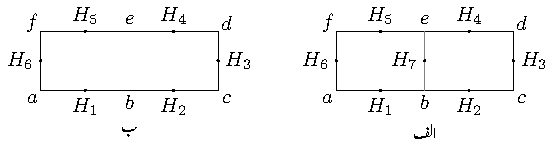
\includegraphics{figMagneticStokesTheorem}
\caption{چھوٹے رقبوں کے گرد لکیری تکمل پورے رقبے کے گرد لکیری تکمل کے برابر ہے۔}
\label{شکل_مقناطیسی_مسئلہ_سٹوکس}
\end{figure}

دائیں رقبے کے لکیری تکمل میں \عددیء{\kvec{H}_7 \cdot \Delta\kvec{L}_{be}=-\kvec{H}_7 \cdot \Delta\kvec{L}_{eb}} لکھ کر دونوں رقبوں کے لکیری تکمل جمع کرتے ہوئے
\begin{align*}
\oint \kvec{H} \cdot \dif \kvec{L}_B+\oint \kvec{H} \cdot \dif \kvec{L}_D&\overset{.}{=} \kvec{H}_1 \cdot \Delta\kvec{L}_{ba}+\kvec{H}_2 \cdot \Delta\kvec{L}_{cb}+ \kvec{H}_3 \cdot \Delta\kvec{L}_{dc}+ \kvec{H}_4 \cdot \Delta\kvec{L}_{ed}+ \kvec{H}_5 \cdot \Delta\kvec{L}_{fe}+ \kvec{H}_6 \cdot \Delta\kvec{L}_{af}\\
&\overset{.}{=}\left(\nabla \times \kvec{H}_B \right) \cdot  \Delta \kvec{S}_B+\left(\nabla \times \kvec{H}_D \right) \cdot  \Delta \kvec{S}_D
\end{align*}
حاصل ہوتا ہے۔آپ دیکھ سکتے ہیں کہ چھوٹے رقبوں کے مشترک طرف \عددیء{\Delta L_{be}} پر دونوں  کے لکیری تکمل آپس میں کٹ گئے ہیں۔یہاں پہلی مساوات پورے رقبے کے گرد لکیری تکمل کے برابر ہے جو شکل \حوالہ{شکل_مقناطیسی_مسئلہ_سٹوکس}-ب کو دیکھ کر لکھی جا سکتی ہے۔
\begin{figure}
\centering
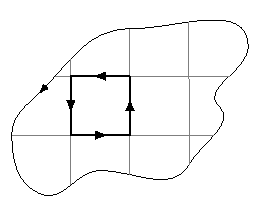
\includegraphics{figMagneticStokesTheoremLargerArea}
\caption{کسی بھی بڑے رقبے کو انتہائی چھوٹے رقبوں میں تقسیم کرتے ہوئے ہر کے گرد لکیری تکمل لیں۔ان تمام کا مجموعہ پورے رقبے کے سرحد پر لکیری تکمل کے برابر ہو گا۔}
\label{شکل_مقناطیسی_سٹوکس_بڑا_رقبہ}
\end{figure}
ہم نے شکل \حوالہ{شکل_مقناطیسی_مسئلہ_سٹوکس}-الف میں رقبے کے صرف دو ٹکڑے لئے۔آپ دیکھ سکتے ہیں کہ رقبے کے زیادہ ٹکڑے کرتے ہوئے  بھی یہی طریقہ کار استعمال کیا جا سکتا ہے۔  اس طرح اگر کسی بھی بڑے رقبے کو انتہائی چھوٹے چھوٹے  رقبوں میں تقسیم کرتے ہوئے ہر ایک کے گرد لکیری تکمل لیا جائے  تو ان کا مجموعہ  پورے رقبے کی سرحد پر گھومتے لکیری تکمل کے برابر ہو گا۔شکل \حوالہ{شکل_مقناطیسی_سٹوکس_بڑا_رقبہ} میں بڑے رقبے کو چھوٹے حصوں میں تقسیم کیا دکھایا گیا ہے۔ہر دو جڑے چھوٹے رقبوں کے مشترکہ طرف پر لکیری تکمل آپس میں کٹ جائیں گے۔ یوں تمام چھوٹے رقبوں کے لکیری تکمل کے مجموعے کو بڑے رقبے کا لکیری تکمل لیتے ہوئے اور تمام چھوٹے رقبوں کے \عددیء{\left(\nabla \times \kvec{H}_B \right) \cdot  \Delta \kvec{S}} کے مجموعے کو تکمل کی شکل میں لکھتے ہوئے
\begin{align}\label{مساوات_مقناطیسی_سٹوکس_مساوات}
\oint \kvec{H} \cdot \dif \kvec{L} =\int_S \left(\nabla \times \kvec{H}_B \right) \cdot  \dif \kvec{S}
\end{align}
لکھا جا سکتا ہے جہاں \عددیء{\dif \kvec{L}} کو صرف بڑے رقبے \عددیء{S} کی سرحد پر لیا جاتا ہے۔

اگرچہ ہم نے مساوات \حوالہ{مساوات_مقناطیسی_سٹوکس_مساوات} مقناطیسی میدان کے لئے حاصل کیا، درحقیقت یہ ایک عمومی مساوات ہے جو کسی بھی سمتی میدان کے لئے درست ہے۔یہ مساوات \اصطلاح{مسئلہ سٹوکس}\فرہنگ{مسئلہ سٹوکس}\حاشیہب{Stokes theorem}\فرہنگ{Stokes theorem} بیان کرتا ہے۔

مسئلہ سٹوکس سے ایمپیئر کا دوری قانون باآسانی حاصل ہوتا ہے۔ایسا کرنے کی خاطر \عددیء{\nabla \times \kvec{H}=\kvec{J}}  کے دونوں اطراف کا \عددیء{\dif \kvec{S}} کے ساتھ غیر سمتی ضرب لیتے ہوئے دونوں اطراف کھلی سطح \عددیء{S} پر سطحی تکمل لیتے  ہوئے مسئلہ سٹوکس کا استعمال کریں گے۔ 
\begin{align*}
\int_S \left(\nabla \times \kvec{H} \right) \cdot \dif \kvec{S}=\int_S \kvec{J} \cdot \dif \kvec{S}=\oint \kvec{H} \cdot \dif \kvec{L}
\end{align*}
کثافت برقی رو کی سطحی تکمل سطح \عددیء{S} سے گزرتی برقی رو کے برابر ہے لہٰذا مندرجہ بالا سے
\begin{align*}
\oint \kvec{H} \cdot \dif \kvec{L}=I
\end{align*}
حاصل ہوتا ہے جو ایمپیئر کا دوری قانون ہے۔ایمپیئر کے دوری قانون کے اس مختصر حصول سے یہ حقیقت بھی واضح ہوتی ہے کہ \عددیء{I} ان تمام سطحوں سے گزرتی برقی رو ہے جن کی سرحد تکمل میں استعمال بند راہ ہے۔

مسئلہ سٹوکس  سطحی تکمل  اور بند لکیری تکمل کے مابین تعلق بیان کرتا ہے۔آپ کو یاد ہو گا کہ مسئلہ پھیلاو حجمی تکمل اور بند سطحی تکمل کے مابین تعلق بیان کرتا ہے۔یہ دونوں مسئلے عمومی سمتیاتی ثبوت پیش کرنے میں اہم کردار ادا کرتے ہیں۔آئیں ایسی ایک مثال دیکھتے ہیں جس میں ہم \عددیء{\nabla \cdot \nabla \times \kvec{A}} کو بیان کرنے  کا مختلف طریقہ حاصل کرنے کی کوشش کرتے ہیں  جہاں \عددیء{\kvec{A}} کوئی بھی عمومی سمتی میدان ہو سکتا ہے۔

شروع کرنے سے پہلے یاد رہے کہ گردش کا حاصل جواب سمتیہ ہوتا ہے جبکہ پھیلاو کا حاصل جواب غیر سمتی ہوتا ہے۔کسی بھی عمومی سمتیہ میدان \عددیء{\kvec{A}} کا گردش \عددیء{\nabla \times \kvec{A}} بھی سمتیہ ہو گا جبکہ اس گردش کا پھیلاو \عددیء{\nabla \cdot \nabla \times \kvec{A}} غیر سمتی ہو گا جسے ہم \عددیء{T} کہتے ہیں یعنی
\begin{align*}
\nabla \cdot \nabla \times \kvec{A}=T
\end{align*}
دونوں اطراف کا حجمی تکمل لیتے ہیں۔
\begin{align*}
\int_{\textrm{حجم}}\left(\nabla \cdot \nabla \times \kvec{A}\right) \dif h=\int_{\textrm{حجم}}T \dif h
\end{align*}
بائیں ہاتھ پر مسئلہ پھیلاو لاگو کرتے ہوئے
\begin{align*}
\oint_S\left(\nabla \times \kvec{A}\right) \cdot \dif \kvec{S}=\int_{\textrm{حجم}}T \dif h
\end{align*}
لکھا جا سکتا ہے۔اس مساوات کا بایاں ہاتھ حجم  کو گھیرتے بند سطح پر \عددیء{\nabla \times \kvec{A}} کا تکمل ہے۔مسئلہ سٹوکس کسی بھی سطح پر سطحی تکمل اور اس سطح کے سرحد پر لکیری تکمل کا تعلق بیان کرتا ہے۔یوں مندرجہ بالا مساوات کے بائیں ہاتھ میں اگر سطح کو تھیلا سمجھا جائے تو تھیلے کا منہ سطح کی سرحد ہو گا جس پر لکیری تکمل لیا جائے گا۔جیسے جیسے تھیلے کے منہ کو چھوٹا کیا جائے ویسے ویسے تھیلا بند سطح کی شکل اختیار کرے گا جبکہ سطح کی سرحد  چھوٹی سے چھوٹی ہوتی جائے گی حتٰی کہ جب تھیلے کا منہ مکمل بند ہو جائے تو تھیلا مکمل بند سطح ہو گا جبکہ اس کی سرحد صفر کے برابر ہو گی۔صفر لمبائی کے راہ پر تکمل صفر کے برابر ہوتا ہے یعنی
\begin{align*}
\int_0^0 \kvec{A} \cdot \dif \kvec{L}=0
\end{align*}
یوں 
\begin{align*}
\int_{\textrm{حجم}} T \dif h=0
\end{align*}
حاصل ہوتا ہے۔چونکہ یہ مساوات کسی بھی حجم کے لئے درست ہے لہٰذا یہ تفرقی حجم \عددیء{\dif h} کے لئے بھی درست ہے یعنی
\begin{align*}
T \dif h=0
\end{align*}
جس سے
\begin{align*}
T=0
\end{align*}
یا
\begin{align}\label{مساوات_مقناطیسی_گردش_کی_پھیلاو_صفر_ہے}
\nabla \cdot \nabla \times \kvec{A}=0
\end{align}
حاصل ہوتا ہے۔مساوات \حوالہ{مساوات_مقناطیسی_گردش_کی_پھیلاو_صفر_ہے} انتہائی اہم ثبوت ہے جس کے تحت کسی بھی عمومی سمتی میدان کے گردش کا پھیلا صفر کے برابر ہوتا ہے۔اس ثبوت کو مندرجہ ذیل مثال میں کارتیسی محدد استعمال کرتے ہوئے بھی حاصل کیا گیا ہے۔
%================================
\ابتدا{مثال}\شناخت{مثال_مقناطیسی_گردش_کا_پھیلاو_صفر}
کسی بھی عمومی سمتی میدان \عددیء{\kvec{A}=A_x\ax+A_y\ay+A_z\az} کا گردش اور گردش کا پھیلا کارتیسی محدد میں حاصل کرتے ہوئے ثابت کریں کہ گردش کا پھیلاو صفر کے برابر ہو گا۔

حل:پہلے گردش حاصل کرتے ہیں
\begin{align*}
\nabla \times \kvec{A}=\left(\frac{\partial A_z}{\partial y}-\frac{\partial A_y}{\partial z} \right)\ax+\left(\frac{\partial A_x}{\partial z}-\frac{\partial A_z}{\partial x} \right)\ay+\left(\frac{\partial A_y}{\partial x}-\frac{\partial A_x}{\partial y} \right)\az
\end{align*}
جس کا پھیلاو
\begin{align*}
\nabla \cdot \nabla \times \kvec{A}=\frac{\partial^2 A_z}{\partial x \partial y}-\frac{\partial^2 A_y}{\partial x \partial z}+\frac{\partial^2 A_x}{\partial y \partial z}-\frac{\partial^2 A_z}{\partial y \partial x}+\frac{\partial^2 A_y}{\partial z \partial x}-\frac{\partial^2 A_x}{\partial z \partial y}=0
\end{align*}
کے برابر ہے جہاں \عددیء{\frac{\partial^2 A_z}{\partial x \partial y}} اور \عددیء{-\frac{\partial^2 A_z}{\partial y \partial x}} کی طرح بقایا اجزاء بھی آپس میں کٹ جاتے ہیں۔
\انتہا{مثال}
%=====================

ساکن مقناطیسی میدان یعنی وقت کے ساتھ تبدیل نہ ہوتے مقناطیسی میدان کے لئے ایمپیئر کے دوری قانون کی نقطہ شکل
\begin{align*}
\nabla \times \kvec{H}=\kvec{J}
\end{align*}
ہے۔اس مساوات کے دونوں اطراف کا پھیلاو حاصل کرتے ہوئے
\begin{align*}
\nabla \cdot \nabla \times \kvec{H}=\nabla \cdot \kvec{J}
\end{align*}
لکھا جا سکتا ہے۔مساوات \حوالہ{مساوات_مقناطیسی_گردش_کی_پھیلاو_صفر_ہے} کے تحت گردش کا پھیلاو صفر کے برابر ہوتا ہے لہٰذا
\begin{align}\label{مساوات_مقناطیسی_استمراری_مساوات}
\nabla \cdot \kvec{J}=0
\end{align}
ہو گا۔اس سے ظاہر ہے کہ ساکن مقناطیسی میدان صرف ایسی برقی رو سے حاصل ہوتا ہے  جس کے لئے مساوات \حوالہ{مساوات_مقناطیسی_استمراری_مساوات} درست ہو۔یہی نتیجہ ہم پہلے بھی مساوات \حوالہ{مساوات_مقناطیسی_صرف_مکمل_بند_راہ} میں حاصل کر چکے ہیں جہاں ہم دیکھ چکے کہ \عددیء{\nabla \cdot \kvec{J}=0} سے مراد بند راہ سے کل صفر یک سمتی برقی رو کا گزرنا ہے۔

\حصہ{مقناطیسی بہاو اور کثافت مقناطیسی بہاو}
خالی خلاء میں کثافت مقناطیسی بہاو \عددیء{\kvec{B}} کی تعریف
\begin{align}\label{مساوات_مقناطیسی_میدان_بالمقابل_شدت}
\kvec{B}=\mu_0 \kvec{H}
\end{align}
ہے جہاں \عددیء{\kvec{B}} کی اکائی ویبر فی مربع میٹر \عددیء{\si{\weber \per \meter^2}} ہے جسے \اصطلاح{ٹسلا}\فرہنگ{ٹسلا}\حاشیہب{Tesla}\فرہنگ{Tesla} پکارا اور \عددیء{\si{\tesla}} سے ظاہر کیا جاتا ہے۔ اس مساوات میں \عددیء{\mu_0} خالی خلاء کا \اصطلاح{مقناطیسی مستقل}\فرہنگ{مقناطیسی مستقل}\حاشیہب{magnetic constant, permeability}\فرہنگ{magnetic constant}\فرہنگ{permeability} ہے جسے ہینری فی میٹر \عددیء{\si{\henry \per \meter}} میں ناپا جاتا ہے۔خالی خلاء میں
\begin{align}
\mu_0=4\pi \times 10^{-7} \si{\henry \per \meter}
\end{align}
کے برابر ہے۔

چونکہ \عددیء{\kvec{H}} کی اکائی ایمپیئر فی میٹر ہے لہٰذا ویبر کی اکائی ہینری ضرب ایمپیئر ہے۔ہینری کو اکائی تصور کرتے ہوئے ہم دیکھتے ہیں کہ ہینری ضرب ایمپیئر کو ویبر لکھا جاتا ہے۔وقت کے ساتھ بدلتے میدان پر غور کے دوران ہم دیکھیں گے کہ ویبر سے مراد وولٹ ضرب سیکنڈ بھی لیا جا سکتا ہے۔ 

خالی خلاء میں کثافت برقی بہاو \عددیء{\kvec{D}} اور برقی میدان کی شدت \عددیء{\kvec{E}} کا تعلق
\begin{align*}
\kvec{D}=\epsilon_0 \kvec{E}
\end{align*}
ہو بہو مساوات \حوالہ{مساوات_مقناطیسی_میدان_بالمقابل_شدت} کی طرح ہے۔کثافت برقی بہاو کا سطحی تکمل برقی بہاو \عددیء{\psi} دیتا ہے۔
\begin{align*}
\psi=\int_S \kvec{D} \cdot \dif \kvec{S}
\end{align*}
کسی بھی بند سطح سے گزرتی برقی بہاو اس سطح میں گھیرے بار \عددیء{Q} کے برابر ہوتا ہے۔
\begin{align*}
\psi=\oint_S \kvec{D} \cdot \dif \kvec{S}=Q
\end{align*}
مثبت بار سے برقی بہاو کا اخراج ہوتا ہے جبکہ منفی بار پر برقی بہاو کا اختتام ہوتا ہے۔یوں برقی بہاو کا منبع برقی بار ہے۔مقناطیسی قطب ہر صورت جوڑی کی شکل میں پائے جاتے ہیں۔آج تک تنہا مقناطیسی قطب نہیں پایا گیا۔یوں آج تک ایسی صورت دیکھنے کو نہیں ملی جہاں تنہا مقناطیسی قطب سے مقناطیسی بہاو کا اخراج ہو یا مقناطیسی بہاو اس پر اختتام پذیر ہو۔ مقناطیسی بہاو کا منبع برقی رو ہے۔ یاد رہے کہ نا تو مقناطیسی بہاو اس برقی رو سے خارج اور نا ہی اس پر اختتام پذیر ہوتی ہے بلکہ یہ بند دائرے کی شکل میں برقی رو کو گھیرتی ہے۔کثافت مقناطیسی بہاو کا سطحی تکمل \اصطلاح{مقناطیسی بہاو}\فرہنگ{مقناطیسی بہاو}\حاشیہب{magnetic flux}\فرہنگ{magnetic flux} \عددیء{\Phi} دیتا ہے جسے \اصطلاح{ویبر}\فرہنگ{ویبر}\فرہنگ{Weber}\حاشیہب{Weber} \عددیء{\si{\weber}} میں ناپا جاتا ہے۔
\begin{align}
\Phi=\int_S \kvec{B} \cdot \dif \kvec{S} \quad \quad \si{\weber}
\end{align} 
چونکہ مقناطیسی بہاو بند دائرہ بناتا ہے لہٰذا کسی بھی بند سطح میں جتنا مقناطیسی بہاو داخل ہوتا ہے، اتنا ہی مقناطیسی بہاو اس سطح سے خارج بھی ہوتا ہے لہٰذا کسی بھی بند سطح پر مقناطیسی بہاو کا تکمل صفر کے برابر ہو گا۔
\begin{align}\label{مساوات_مقناطیسی_مقناطیسی_بہاو_بند_سطح}
\oint_S \kvec{B} \cdot \dif \kvec{S}=0
\end{align}
مسئلہ پھیلاو کے استعمال سے مندرجہ بالا مساوات سے
\begin{align}\label{مساوات_مقناطیسی_مقناطیسی_بہاو_پھیلاو}
\nabla \cdot \kvec{B}=0
\end{align}
حاصل ہوتا ہے۔

ہم نے مساوات \حوالہ{مساوات_مقناطیسی_مقناطیسی_بہاو_بند_سطح} کو ثابت نہیں کیا بلکہ حقیقت کو سامنے رکھتے ہوئے اسے لکھا ہے۔اس کو آگے ثابت کیا جائے گا۔فی الحال اس کو قبول کر لیں اور یوں مساوات  \حوالہ{مساوات_مقناطیسی_مقناطیسی_بہاو_پھیلاو} کو بھی درست تصور کریں۔

ساکن مقناطیسی اور ساکن برقی میدان کے لئے مساوات \حوالہ{مساوات_مقناطیسی_مقناطیسی_بہاو_پھیلاو}  میکس ویل کی چوتھی اور آخری مساوات ہے۔ان تمام کو یہاں دوبارہ پیش کرتے ہیں۔
\begin{gather}
\begin{aligned}\label{مساوات_مقناطیسی_میکس_ویل_نقطہ_اشکال}
\nabla \cdot \kvec{D}&=\rho\\
\nabla \times \kvec{E}&=0\\
\nabla \times \kvec{H}&=\kvec{J}\\
\nabla \cdot \kvec{B}&=0
\end{aligned}
\end{gather}
ان کے ساتھ
\begin{gather}
\begin{aligned}
\kvec{D}&=\epsilon_0 \kvec{E}\\
\kvec{B}&=\mu_0 \kvec{H}
\end{aligned}
\end{gather}
کو بھی شامل کرتے ہیں۔ہم برقی میدان کی شدت اور ساکن برقی دباو کا تعلق بھی پیش کرتے ہیں۔
\begin{align}
\kvec{E}=-\nabla V
\end{align}

مساوات \حوالہ{مساوات_مقناطیسی_میکس_ویل_نقطہ_اشکال} برقی اور مقناطیسی میدان کے پھیلاو اور گردش بیان کرتے ہیں جو ان میدان کی خاصیت کے نقطہ اشکال ہیں۔ان کی تکمل اشکال مندرجہ ذیل ہیں۔
\begin{gather}
\begin{aligned}
\oint_S \kvec{D} \cdot \dif \kvec{S}&=Q=\int_{\textrm{حجم}} \rho_h \dif h\\
\oint \kvec{E} \cdot \dif \kvec{L}&=0\\
\oint \kvec{H} \cdot \dif \kvec{L}&=I=\int_S \kvec{J} \cdot \dif \kvec{S}\\
\oint_S \kvec{B} \cdot \dif \kvec{S}&=0
\end{aligned}
\end{gather}
ہم جلد ساکن مقناطیسی میدان کے مقناطیسی دباو پر بھی غور کریں گے۔ہم نے برقی میدان پر غور کے دوران موصل اجزاء کے اثر کو بھی تقطیب \عددیء{\kvec{P}} کی صورت میں شامل کیا۔ایسا کرتے ہوئے جزو برقی مستقل کا سہارا لیا گیا۔اگلے باب میں اسی طرح دیگر اجزاء کا مقناطیسی میدان پر اثر دیکھا جائے گا۔

آئیں مقناطیسی بہاو اور کثافت مقناطیسی بہاو کا استعمال ہم محوری تار کے اندر بہاو کے مثال کی صورت میں دیکھیں۔ایسی ہم محوری تار جسے شکل \حوالہ{شکل_مقناطیسی_ہم_محوری_تار} میں دکھایا گیا ہے میں مقناطیسی شدت
\begin{align*}
H_{\phi}=\frac{I}{2\pi \rho} \quad \quad (\rho_1 < \rho < \rho_2)
\end{align*}
ہم پہلے حاصل کر چکے ہیں۔ یوں کثافت مقناطیسی بہاو
\begin{align*}
\kvec{B}=\mu_0 \kvec{H}=\frac{\mu_0 I}{2\pi \rho} \aphi
\end{align*}
ہو گا۔اندرونی اور بیرونی تار کے درمیان مقناطیسی بہاو وہی ہو گا جو ان تاروں کے درمیان رداسی سیدھی سطح سے گزرے گا۔تار کو \عددیء{z} محدد پر تصور کرتے ہوئے \عددیء{z=0} تا \عددیء{z=d} تک رداسی سطح سے گزرتی مقناطیسی بہاو
\begin{align*}
\Phi=\int_S \kvec{B} \cdot \dif \kvec{S}=\int_{0}^{d} \int_{\rho_1}^{\rho_2} \frac{\mu_0 I}{2\pi \rho} \aphi \cdot (\dif \rho \dif z \aphi)
\end{align*}
یعنی
\begin{align}
\Phi=\frac{\mu_0 I d}{2\pi} \ln \frac{\rho_2}{\rho_1}
\end{align}
ہو گی۔ یہ مساوات آگے جا کر ہم محوری تار کے امالہ کے حصول میں کام آئے گی۔
%=================

\ابتدا{مشق}
تانبے کی تار کو پانی سے ٹھنڈا کرتے ہوئے اس میں زیادہ کثافت برقی رو گزاری جا سکتی ہے۔ایک ایسی ہم محوری تار جس کے اندرونی تار کا اندرونی رداس \عددیء{\SI{25}{\milli \meter}} جبکہ اس کا بیرونی رداس \عددیء{\SI{28}{\milli \meter}} ہے اور جس کے بیرونی تار کا اندرونی رداس \عددیء{\SI{35}{\milli\meter}} اور بیرونی رداس \عددیء{\SI{37}{\milli \meter}} ہے میں \عددیء{\SI{10000}{\ampere}} کا یک سمتی برقی رو تاروں میں الٹ سمت میں گزر رہی ہے۔ٹھنڈا پانی اندرونی تار کے اندر اور تاروں کے درمیان فاصلے سے گزار کر انہیں ٹھنڈا رکھا جاتا ہے۔ دونوں تاروں کے اندر اور ان کے مابین \عددیء{\kvec{H}} اور \عددیء{\kvec{B}} حاصل کرنے کے بعد \عددیء{\SI{1}{\meter}}  لمبائی کے  لئے  دونوں تاروں کے اندر اور ان کے مابین  مقناطیسی بہاو حاصل کریں۔

جوابات: اندرونی تار میں \عددیء{J=\SI{20}{\ampere \per \milli \meter \squared}} اور \عددیء{\Phi=\SI{109}{\micro \weber}} ہیں۔بیرونی تار میں \عددیء{J=\SI{22.1}{\ampere \per \milli \meter \squared}} اور \عددیء{\Phi=\SI{56.6}{\micro \weber}} ہیں۔تاروں کے درمیانی فاصلے میں \عددیء{\Phi=\SI{446}{\micro\weber}} ہے۔
\انتہا{مشق}
%=================
\ابتدا{مشق}\شناخت{مشق_مقناطیسی_دائرے_میں_رو}
\عددیء{z=0} سطح پر \عددیء{\rho} رداس کے گول بند دائرے میں \عددیء{I} برقی رو گزر رہی ہے۔گول دائرے کا مرکز کارتیسی محدد کے \عددیء{(0,0,0)} پر ہے۔اگر مثبت \عددیء{z} جانب  سے دیکھا جائے تو برقی رو گھڑی کے الٹ سمت میں گھوم رہی ہے۔بایوٹ سیوارٹ کے قانون سے دائرے کے عین وسط میں \عددیء{\kvec{H}} حاصل کریں۔

جواب: \عددیء{\kvec{H}=\tfrac{I}{2\rho}\az}
\انتہا{مشق}
%===============

مندرجہ بالا مشق میں آپ نے دائرے کے مرکز پر مقناطیسی میدان حاصل کیا۔یہی طریقہ استعمال کرتے ہوئے دائرے کے محور پر کسی بھی نقطے پر مقناطیسی میدان حاصل کیا جا سکتا ہے۔البتہ جیسے ہی محور سے ہٹ کر مقناطیسی میدان مطلوب ہو مسئلہ خاصہ مشکل ہو جاتا ہے۔مندرجہ ذیل مثال میں اس حقیقت کو سامنے رکھا جائے گا کہ محور سے ہٹ کر برقی رو گزارتے گول دائرے کا مقناطیسی میدان حاصل کرنا کیوں ممکن نہیں ہو گا۔اس کے بعد  اس مسئلے کا \اصطلاح{عددی حل}\حاشیہب{numerical solution} حاصل کرنا دکھایا جائے گا۔کمپیوٹر استعمال کرتے ہوئے کسی بھی مسئلے کا عددی حل حاصل کیا جا سکتا ہے۔

\ابتدا{مثال}
شکل \حوالہ{شکل_مقناطیسی_دائرہ_محور_سے_ہٹ_کر} میں \عددیء{x=0} سطح یعنی \عددیء{yz} سطح پر نقطہ \عددیء{N(0,y,z)} پر گول بند دائرے میں یک سمتی برقی رو سے پیدا مقناطیسی میدان کی شدت حاصل کریں۔ 
\begin{figure}
\centering
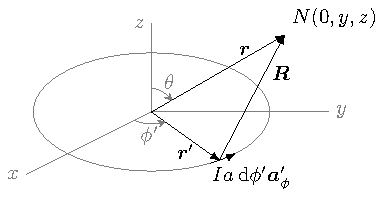
\includegraphics{figMagneticOffAxisFieldOfCurrentRing}
\caption{گول بند دائرے میں یک سمتی برقی رو کا محور سے ہٹ کر مقناطیسی میدان۔}
\label{شکل_مقناطیسی_دائرہ_محور_سے_ہٹ_کر}
\end{figure}

حل:رداس \عددیء{a} کے گول دائرے پر نقطہ \عددیء{N'(a,\tfrac{\pi}{2},\phi')} پر چھوٹی سمتی لمبائی کو \عددیء{\dif \kvec{L}'=a \dif \phi' \aphi'} لکھا جا سکتا ہے جہاں اکائی سمتیہ \عددیء{\aphi'} کو کارتیسی محدد میں
\begin{align*}
\aphi'=-\sin \phi' \ax+\cos \phi' \ay 
\end{align*}
لکھا جا سکتا ہے۔یوں
\begin{align*}
\dif \kvec{L}'= a \dif \phi' \left(-\sin \phi' \ax+\cos \phi' \ay  \right)
\end{align*}
لکھا جا سکتا ہے۔یہ چھوٹی لمبائی خود \عددیء{(a\cos \phi',a\sin \phi')} پر پائی جاتی ہے یعنی
\begin{align*}
\kvec{r}'=a \arho'=a\cos \phi' \ax+a\sin \phi' \ay
\end{align*}
کے برابر ہے۔نقطہ \عددیء{N} کا مقام کارتیسی محدد میں
\begin{align*}
\kvec{r}=y\ay+z\az
\end{align*}
ہے۔یوں
\begin{align*}
\kvec{R}=\kvec{r}-\kvec{r}'=-a\cos \phi' \ax+(y-a\sin \phi')\ay+z\az
\end{align*}
لکھتے ہوئے
\begin{align*}
\abs{\kvec{R}}=R&=\sqrt{(-a\cos \phi')^2+(y-a\sin \phi')^2+z^2}\\
&=\sqrt{a^2+y^2+z^2-2 a y\sin \phi'}
\end{align*}
اور
\begin{align*}
\aR=\frac{\kvec{R}}{\abs{\kvec{R}}}=\frac{-a\cos \phi' \ax+(y-a\sin \phi')\ay+z\az}{\sqrt{a^2+y^2+z^2-2 a y\sin \phi'}}
\end{align*}
حاصل ہوتے ہیں۔بایوٹ سیوارٹ قانون میں \عددیء{\aR=\tfrac{\kvec{R}}{R}}  پر کرتے ہوئے 
\begin{align*}
\kvec{H}=\oint \frac{I \dif \kvec{L}' \times \kvec{R}}{4\pi R^3}
\end{align*}
لکھا جا سکتا ہے۔آئیں پہلے \عددیء{\dif \kvec{L}' \times \kvec{R}} کی سادہ شکل حاصل کریں۔
\begin{align*}
\dif \kvec{L}' \times \kvec{R}&=a \dif \phi' \left(-\sin \phi' \ax+\cos \phi' \ay  \right) \times \left[-a\cos \phi' \ax+(y-a\sin \phi')\ay+z\az \right]\\
&=a \dif \phi' \left[z\cos \phi' \ax+z\sin \phi' \ay+(a-y\sin\phi')\az \right]
\end{align*}
یوں بایوٹ سیوارٹ کے قانون کو
\begin{align*}
\kvec{H}=\frac{a I}{4\pi}\int \limits_{0}^{2\pi} \frac{z\cos \phi' \ax+z\sin \phi' \ay+(a-y\sin\phi')\az}{\left(a^2+y^2+z^2-2 a y\sin \phi'\right)^{\frac{3}{2}}} \dif \phi'
\end{align*}
لکھا جا سکتا ہے۔اس مساوات میں \عددیء{H_x} جزو صفر کے برابر ہے۔یہ حقیقت سیدھی منطق سے ثابت ہوتی ہے۔کسی بھی زاویہ \عددیء{\phi'} پر چھوٹی لمبائی سے پیدا میدان کو زاویہ \عددیء{{\pi-\phi'}} پر چھوٹی لمبائی کا میدان ختم کرتا ہے۔یوں یہ جزو صفر کے برابر ہے۔یہی نتیجہ تحلیلی طور پر حاصل کرنے کی خاطر، \عددیء{H_x} جزو میں نیا متغیرہ
 \عددیء{{w=a^2+y^2+z^2-2ay\sin\phi'}} پر کرتے ہوئے تکمل
\begin{align*}
H_x=\frac{a I}{4\pi}\int \limits_{0}^{2\pi} \frac{z\cos \phi' \dif \phi'}{\left(a^2+y^2+z^2-2 a y\sin \phi'\right)^{\frac{3}{2}}}=0
\end{align*}
سے حاصل کیا جا سکتا ہے۔بقایا دو اجزاء
\begin{gather}
\begin{aligned}\label{مساوات_مقناطیسی_دائرے_کا_محور_سے_دور_اجزاء}
H_y&=\frac{aI}{4\pi}\int\limits_0^{2\pi} \frac{z\sin \phi' \dif \phi'}{\left(a^2+y^2+z^2-2 a y\sin \phi'\right)^{\frac{3}{2}}}\\
H_z&=\frac{a I}{4\pi}\int \limits_{0}^{2\pi} \frac{(a-y\sin\phi') \dif \phi'}{\left(a^2+y^2+z^2-2 a y\sin \phi'\right)^{\frac{3}{2}}} 
\end{aligned}
\end{gather}
ہیں۔یہ دونوں \اصطلاح{بیضوی تکمل}\فرہنگ{تکمل!بیضوی}\حاشیہب{elliptic integral}\فرہنگ{integral!elliptic} ہیں جنہیں الجبرائی طریقے سے حل کرنا ممکن نہیں ہے۔
\انتہا{مثال}
%======================
\اصطلاح{بیضوی تکمل} کا \اصطلاح{عددی حل}\فرہنگ{عددی حل}\حاشیہب{numerical solution}\فرہنگ{numerical solution} بذریعہ کمپیوٹر حاصل کیا جاتا ہے۔آئیں قلم و کاغذ استعمال کرتے ہوئے بیضوی تکمل کا عددی حل حاصل کریں۔
%====================

\ابتدا{مثال}\شناخت{مثال_مقناطیسی_دائرہ_برقی_رو_کے_بیضوی_تکمل}
مندرجہ بالا مثال میں \عددیء{H_y} اور \عددیء{H_z} کے حل  \اصطلاح{بیضوی تکمل}  کی صورت میں حاصل ہوئے۔نقطہ \عددیء{N(0,a,a)} پر \عددیء{H_y} کا \اصطلاح{عددی حل} حاصل کریں۔
\begin{figure}
\centering
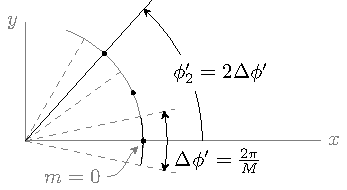
\includegraphics{figMagneticOffAxisFieldOfCurrentRingNumericalSolution}
\caption{تکمل کے راہ کو متعدد چھوٹے ٹکڑوں میں تقسیم کیا گیا ہے۔}
\label{شکل_مقناطیسی_عددی_حل_دائرہ_برقی_رو}
\end{figure}

حل:اس نقطے پر 
\begin{align*}
H_y&=\frac{aI}{4\pi}\int\limits_0^{2\pi} \frac{a\sin \phi' \dif \phi'}{\left(a^2+a^2+a^2-2 a^2\sin \phi'\right)^{\frac{3}{2}}}\\
&=\frac{I}{4\pi a}\int\limits_0^{2\pi} \frac{\sin \phi' \dif \phi'}{\left(3-2\sin \phi'\right)^{\frac{3}{2}}}
\end{align*}
لکھا جائے گا۔اس تکمل کو مجموعے کی شکل میں لکھا جا سکتا ہے۔شکل \حوالہ{شکل_مقناطیسی_عددی_حل_دائرہ_برقی_رو} کو دیکھ کر آگے پڑھیں۔تکمل کے راہ کو \عددیء{M} برابر ٹکڑوں میں تقسیم کرتے  ہوئے ہر ٹکڑا پر \عددیء{\Delta \phi'=\tfrac{2\pi}{M}} کے برابر ہو گا۔ان ٹکڑوں کی گنتی کا حساب ہم \عددیء{m} سے رکھتے ہیں جہاں \عددیء{m} کی قیمت \عددیء{0} تا \عددیء{(M-1)} ہے۔یوں پہلے ٹکڑے کو \عددیء{m=0} سے ظاہر کیا جائے گا اور اس ٹکڑے کے عین وسط میں زاویہ \عددیء{\phi_0'=0} ہو گا۔شکل میں راہ کے چھوٹے ٹکڑوں کے عین وسط کو نقطوں سے ظاہر کیا گیا ہے۔دوسرے ٹکڑے پر \عددیء{m=1} اور زاویہ \عددیء{\phi_1'=\Delta \phi'=\tfrac{2\pi}{M}} ہو گا۔جیسے شکل میں دکھایا گیا ہے، تیسرے پر \عددیء{m=2} اور زاویہ  \عددیء{\phi_2'=2\Delta \phi'=\tfrac{2\times 2\pi}{M}} ہو گا۔یوں عمومی ٹکڑے \عددیء{m} پر زاویہ
 \عددیء{\phi_m'=m\Delta \phi'=\tfrac{2 m \pi}{M}} ہو گا۔

اگر ان چھوٹے ٹکڑوں پر تفاعل کی قیمت میں تبدیلی کو رد کرنا ممکن ہو تب ہر چھوٹے ٹکڑے پر تکمل تقریباً
\begin{align*}
\Delta H_y&=\frac{I}{4\pi a} \frac{\sin \phi_m' \Delta \phi'}{\left(3-2\sin \phi_m'\right)^{\frac{3}{2}}} \\
&=\frac{I}{4\pi a} \frac{\sin (\frac{2 m \pi}{M}) \frac{2\pi}{M}}{\left(3-2\sin   \frac{2 m \pi}{M}\right)^{\frac{3}{2}}} 
\end{align*}
کے برابر ہو گا۔یوں تمام ٹکڑوں کا مجموعہ
\begin{align*}
H_y= \frac{I}{4\pi a} \frac{2\pi}{M} \sum_{m=0}^{M-1}\frac{\sin  \frac{2 m \pi}{M} }{\left(3-2\sin  \frac{2 m \pi}{M}\right)^{\frac{3}{2}}}
\end{align*}
ہو گا۔جدول \حوالہ{جدول_مقناطیسی_دائرہ_مقناطیسی_شدت_عددی_حل} میں \عددیء{M=10} کی صورت میں \عددیء{m} کے تمام قیمتوں پر حاصل \عددیء{\tfrac{\sin  \frac{2 m \pi}{M}}{\left(3-2\sin  \frac{2 m \pi}{M}\right)^{\frac{3}{2}}}}  اجزاء دئے گئے ہیں۔ان تمام کا مجموعہ
\begin{align*}
H_y&=\frac{I}{4\pi a} \frac{2\pi}{M} \left(0.00000+0.23852 +  0.82674 +  0.82674  + 0.23852  + 0.00000 \right.  \\
& \quad \quad \quad \quad \quad \left.-0.06889  -0.08763  -0.08763  -0.06889\right)\\
&=\frac{I}{4\pi a}\frac{2\pi}{10} (1.8175)\\
&=1.1420 \left(\frac{ I}{4\pi a}\right)
\end{align*}
حاصل ہوتا ہے۔زیادہ سے زیادہ ٹکڑے لیتے ہوئے زیادہ درست جواب حاصل ہوتا ہے۔اگر \عددیء{M=100} کر دیا جائے تب  \عددیء{H_y=\tfrac{1.1433 I}{4\pi a}} حاصل ہوتا ہے۔
\begin{table}
\centering
\begin{tabular}{c c}
$m$& $\frac{\sin  \frac{2 m \pi}{M}}{\left(3-2\sin  \frac{2 m \pi}{M}\right)^{\frac{3}{2}}}$\\[3ex]
\hline
$0$& $0.00000$\\
$1$& $0.23852$\\
$2$&$0.82674 $\\
$3$& $0.82674$\\
$4$& $0.23852$\\
$5$& $0.00000$\\
$6$& $-0.06889$\\
$7$&$-0.08763$\\
$8$& $ -0.08763$\\
$9$& $-0.06889$
\end{tabular}
\caption{دائرے پر برقی رو سے حاصل مقناطیسی میدان کی شدت بذریعہ عددی حل۔}
\label{جدول_مقناطیسی_دائرہ_مقناطیسی_شدت_عددی_حل}
\end{table}

جدول کو دیکھتے ہوئے ظاہر ہے کہ \عددیء{m=0} اور \عددیء{m=5} برابر حصہ ڈالتے ہیں۔اسی طرح \عددیء{m=1} اور \عددیء{m=4} بھی برابر حصہ ڈالتے ہیں۔ان حقائق کو مد نظر رکھتے ہوئے پورے جدول کو حل کرنا درکار نہیں ہے۔درحقیقت موجودہ مثال میں جدول کے صرف پانچ یعنی آدھے خانوں  کا حل درکار ہے۔موجودہ مسئلے میں صرف دس چھوٹے ٹکڑے کرتے ہوئے تقریباً درست جواب حاصل ہوتا ہے۔دس اور سو ٹکڑوں کے جوابات میں صرف
\begin{align*}
\left(\frac{1.1433-1.1420}{1.1433}\right)\times 100=\SI{0.11}{\percent} 
\end{align*}
کا فرق ہے۔
\انتہا{مثال}
%====================
\حصہ{غیر سمتی اور سمتی مقناطیسی دباو}
برقی میدان کے مسائل برقی دباو کے استعمال سے نہایت آسان ہو جاتے ہیں۔گھریلو \عددیء{\SI{220}{\volt}} کے برقی دباو سے آپ بخوبی واقف ہیں۔اگرچہ برقی دباو سے ہمیں روز مرہ زندگی میں عموماً واسطہ پڑتا ہے اور یہ ہمارے لئے ایک حقیقت رکھتا ہے، مقناطیس و برقیات کے میدان میں برقی دباو کی اہمیت صرف اس وجہ سے ہے کہ اس کی مدد سے برقی مسائل باآسانی حل ہو جاتے ہیں۔مثال کے طور پر ہم کسی بھی بار سے پہلے برقی دباو اور پھر برقی دباو سے برقی شدت حاصل کرتے ہیں۔

برقی دباو غیر سمتی مقدار ہے۔ ہم جلد دیکھیں گے کہ برقی دباو کے طرز پر \اصطلاح{غیر سمتی مقناطیسی دباو}\فرہنگ{مقناطیسی دباو!غیر سمتی}\حاشیہب{scalar magnetic potential}\فرہنگ{potential!scalar magnetic} بیان کیا جا سکتا ہے۔البتہ یہ صرف کثافت برقی رو سے پاک مقامات پر قابل بیان ہوتا ہے۔یوں اس کا استعمال ہر جگہ ممکن نہیں ہو گا۔اس کے برعکس \اصطلاح{سمتی مقناطیسی دباو}\فرہنگ{مقناطیسی دباو!سمتی}\حاشیہب{vector magnetic potential}\فرہنگ{potential!vector magnetic} بھی بیان کیا جا سکتا ہے جو انتہائی اہمیت کا حامل ہے۔سمتی مقناطیسی دباو \اصطلاح{اینٹینا}\فرہنگ{اینٹینا}\حاشیہب{antenna}\فرہنگ{antenna}، \اصطلاح{مویج}\فرہنگ{مویج}\حاشیہب{waveguide}\فرہنگ{waveguide} اور مائیکرو ویو چولھے (خرد موج چولھے)\فرہنگ{مائیکرو ویو چولھا}\فرہنگ{خرد موج چولھا}\حاشیہب{microwave oven}\فرہنگ{microwave oven} پر غور کرنے میں مدد دیتا ہے۔یہ وقت کے ساتھ تبدیل ہوتے میدان میں بھی قابل استعمال ہو گا اور یہ ان مقامات پر بھی قابل بیان ہو گا جہاں برقی رو پائی جائے۔آئیں پہلے غیر سمتی مقناطیس دباو دیکھیں۔

برقی دباو اور برقی میدان کی شدت کا تعلق صفحہ \حوالہصفحہ{مساوات_توانائی_ڈھلوان_تعریف_پ} پر مساوات \حوالہ{مساوات_توانائی_ڈھلوان_تعریف_پ} میں بیان کیا گیا ہے۔ہم فرض کرتے ہیں  بالکل اسی طرح غیر سمتی مقناطیسی دباو \عددیء{V _m} کی ڈھلوان منفی مقناطیسی شدت دیتا ہے یعنی
\begin{align*}
\kvec{H}=-\nabla V_m
\end{align*}
یہ نیا تفاعل مقناطیسی میدان کے دیگر تفاعل کے ساتھ ہم آہنگ ہونا چاہیے لہٰذا اسے ایمپیئر کے دوری قانون کے نقطہ صورت پر پورا اترنا ہو گا۔اس طرح
\begin{align}
\nabla \times \kvec{H}=\kvec{J}=\nabla \times \left(-\nabla V_m\right) 
\end{align}
ہو گا۔ البتہ جیسے آپ مشق \حوالہ{مشق_مقناطیسی_ڈھلوان_کی_گردش-صفر} میں دیکھیں گے، کسی بھی متغیرہ کی ڈھلوان کا گردش صفر کے برابر ہوتا ہے۔یوں مقناطیسی میدان کے شدت اور غیر سمتی مقناطیسی دباو کا تعلق صرف اس صورت درست ہو سکتا ہے جب \عددیء{\kvec{J}=0} ہو یعنی
\begin{align}\label{مساوات_مقناطیسی_شدت_غیر_سمتی_دباو}
\kvec{H}=-\nabla V_m \quad \quad (\kvec{J}=0)
\end{align}
اب آپ دیکھ سکتے ہیں کہ غیر مقناطیسی دباو پر لاگو شرط کہ کثافت برقی رو صفر ہونا ضروری ہے ناقابل قبول شرط ہے۔اگرچہ کئی صورتوں میں کثافت برقی رو صفر ہو گی اور \عددیء{V_m} کا استعمال ممکن ہو گا لیکن ہمیں ایسے مسائل بھی درپیش ہوں  گے جہاں کثافت برقی رو صفر نہ ہو گی۔ایسی صورت میں \عددیء{V_m} ہمارے کسی کام کا نہ ہو گا۔ غیر سمتی مقناطیسی دباو \عددیء{V_m} کی تعریف سے ظاہر ہے کہ اسے ایمپیئر میں ناپا جائے گا۔

خالی خلاء میں
\begin{align*}
\nabla \cdot \kvec{B}=\mu_0 \nabla \cdot \kvec{H}=0
\end{align*}
سے
\begin{align*}
\mu_0 \nabla \cdot \left(-\nabla V_m \right)=0
\end{align*}
یا
\begin{align}
\nabla^2 V_m=0 \quad \quad (\kvec{J}=0)
\end{align}
جو لاپلاس مساوات ہے حاصل ہوتا ہے۔یوں غیر سمتی مقناطیسی دباو لاپلاس مساوات پر پورا اترتا ہے۔ہم دیکھیں گے کہ ہر طرف یکساں خاصیت کے مقناطیسی اشیاء میں بھی \عددیء{V_m} لاپلاس مساوات پر پورا اترتا ہے۔یاد رہے کہ \عددیء{V_m} صرف اور صرف کثافت برقی رو سے پاک مقامات پر درست ثابت ہوتا ہے۔

اگلے باب میں \عددیء{V_m} پر تفصیلی غور کیا جائے گا۔یہاں یہ بتلانا ضروری ہے کہ چونکہ مقناطیسی میدان  بقائی میدان نہیں ہے لہٰذا \عددیء{V_m} کی قیمت اٹل نہیں ہو گی۔آپ کو یاد ہو گا کہ برقی میدان میں کسی نقطے کو برقی زمین رکھتے ہوئے کسی دوسرے نقطے پر برقی دباو اٹل قیمت رکھتی ہے۔مقناطیسی میدان میں ایسا ممکن نہیں ہے۔ایسی ایک مثال دیکھنے کی خاطر \عددیء{z} محدد پر رکھی لامحدود لمبائی کے تار پر غور کرتے ہیں جس میں \عددیء{\az} جانب \عددیء{I} برقی رو گزر رہی ہو۔ایسی تار کے گرد جہاں \عددیء{\kvec{J}=0} ہے
\begin{align*}
\kvec{H}=\frac{I}{2\pi \rho} \aphi
\end{align*}
ہو گا اور غیر سمتی مقناطیسی دباو حاصل کیا جا سکتا ہے۔مساوات \حوالہ{مساوات_مقناطیسی_شدت_غیر_سمتی_دباو} اور نلکی محدد میں \عددیء{V_m} کے ڈھلوان کا زاویائی جزو لیتے ہوئے
\begin{align*}
\frac{I}{2\pi \rho} =-\frac{1}{\rho} \frac{\partial V_m}{\partial \phi}
\end{align*}
یا
\begin{align*}
\frac{\partial V_m}{\partial \phi}=-\frac{I}{2\pi}
\end{align*}
سے
\begin{align*}
V_m=-\frac{I}{2\pi}\phi
\end{align*}
حاصل ہوتا ہے جہاں تکمل کے مستقل کو صفر چننا گیا ہے تا کہ \عددیء{\phi=0} پر مقناطیسی زمین ہو۔آپ دیکھ سکتے ہیں کہ \عددیء{\phi=0} پر \عددیء{V_m=0} ہے لہٰذا یہی مقناطیسی زمین ہے۔اب اگر ہم تار کے گرد پورا چکر کاٹیں تو ہم اسی مقناطیسی زمین پر دوبارہ پہنچتے ہیں لیکن مندرجہ بالا مساوات کے تحت \عددیء{\phi=2\pi} پر \عددیء{V_m=-I} کے برابر ہے نا کہ صفر۔تار کے گرد دو چکر کے بعد اسی نقطے پر \عددیء{V_m=-2I} حاصل ہوتا ہے۔آپ دیکھ سکتے ہیں کہ کسی بھی نقطے پر غیر سمتی مقناطیسی دباو کے متعدد قیمتیں ممکن ہیں۔آپ کو یاد ہو گا کہ برقی میدان میں ایک مرتبہ برقی زمین چننے کے بعد کسی بھی ایک نقطے پر ایک ہی برقی دباو کی قیمت حاصل ہوتی ہے۔

آئیں غیر سمتی مقناطیسی دباو کے متعدد قیمتوں کا ممکن ہونا سمجھیں۔ساکن برقی میدان میں
\begin{align*}
\nabla \times \kvec{E}&=0\\
\oint \kvec{E} \cdot \dif \kvec{L}&=0
\end{align*} 
ہوتا ہے لہٰذا دو نقطوں کے مابین لکیری تکمل
\begin{align*}
V_{ab}=-\int_b^a \kvec{E} \cdot \dif \kvec{L}
\end{align*}
کا دارومدار تکمل کے راہ پر منحصر نہیں ہوتا۔ساکن مقناطیسی میدان میں 
\begin{align*}
\nabla \times \kvec{H}=0 \quad \quad (\kvec{J}=0)
\end{align*}
ہوتا ہے لیکن
\begin{align*}
\oint \kvec{H} \cdot \dif \kvec{L}=I
\end{align*}
کے برابر ہوتا ہے اگرچہ تکمل کے راہ پر \عددیء{\kvec{J}=0} ہے۔یوں تکمل لیتے ہوئے جب بھی ایک چکر پورا ہو، تکمل کی قیمت میں \عددیء{I} برابر اضافہ آئے گا۔ہاں اگر تکمل کی راہ صفر برقی رو گھیرے تب غیر سمتی  مقناطیسی دباو بھی ایک قیمت رکھے گا۔ان حقائق کو مدنظر رکھتے ہوئے غیر سمتی مقناطیسی دباو 
\begin{align}
V_{ab}=-\int_{b}^{a} \kvec{H} \cdot \dif \kvec{L} \quad \quad (\textrm{\RL{قیمت راہ پر منحصر ہے}})
\end{align}
بیان کی جاتی ہے۔ہم یہ فیصلہ کر سکتے ہیں کہ غیر سمتی مقناطیسی دباو حاصل کرتے وقت صرف ایک چکر کاٹا جائے گا۔اس شرط پر چلتے ہوئے \عددیء{V_m} ایک قیمت رکھے گا۔یہ آپ مندرجہ بالا مثال سے دیکھ سکتے ہیں یعنی
\begin{align}\label{مساوات_مقناطیسی_غیر_سمتی_دباو_خطہ}
V_m=-\frac{I}{2\pi} \phi \quad \quad (-\pi < \phi \le \pi)
\end{align}
کی صورت میں \عددیء{\phi=0} پر \عددیء{V_m=0} ہی حاصل ہوتا ہے۔اس مساوات میں چکر کی وضاحت ضروری ہے۔صفر زاویہ سے شروع ہو کر اگر زاویہ \عددیء{\phi} مثبت جانب بڑھایا جائے تو \عددیء{\phi=\pi} تک پہنچا جا سکتا ہے۔اس کے برعکس اگر صفر زاویہ سے شروع ہو کر زاویہ \عددیء{\phi} منفی کرتے ہوئے \عددیء{\phi=\pi} تک پہنچنے کی کوشش کی جائے تو ایسا ممکن نہیں ہے۔یوں \عددیء{\phi=\pi} پر \عددیء{V_m} کی ایک عدد قیمت ہو گی۔
%====================
\ابتدا{مشق}\شناخت{مشق_مقناطیسی_ڈھلوان_کی_گردش-صفر}
کارتیسی محدد استعمال کرتے ہوئے مثال \حوالہ{مثال_مقناطیسی_گردش_کا_پھیلاو_صفر} کے طرز پر  ثابت کریں کہ کسی بھی غیر سمتی متغیرہ کے ڈھلوان کی گردش صفر کے برابر ہو گی یعنی
\begin{align}
\nabla \times \left(\nabla V \right)=0
\end{align}

\انتہا{مشق}
%=================

آئیں اب سمتی مقناطیسی دباو پر غور کرتے ہیں۔ہم شروع
\begin{align}\label{مساوات_مقناطیسی_پھیلاو_بہاو_صفر_ہے}
\nabla \cdot \kvec{B}=0
\end{align}
سے کرتے ہیں۔سمتی مقناطیسی دباو کو اس مساوات کے ہم آہنگ ہونا ہو گا۔مساوات \حوالہ{مساوات_مقناطیسی_گردش_کی_پھیلاو_صفر_ہے} میں ہم دیکھ چکے ہیں کہ کسی بھی سمتی متغیرہ کے گردش کا پھیلاو صفر کے برابر ہوتا ہے لہٰذا اگر \عددیء{\kvec{B}} سمتی متغیرہ \عددیء{A} کا گردش
\begin{align}\label{مساوات_مقناطیسی_سمتی_دباو_تعریف}
\kvec{B}=\nabla \times \kvec{A}
\end{align}
 ہو تب بھی \عددیء{\kvec{B}} کا پھیلاو
\begin{align*}
\nabla \cdot \nabla \times \kvec{A}=0
\end{align*}
ہی ہو گا۔ہم مساوات \حوالہ{مساوات_مقناطیسی_سمتی_دباو_تعریف} میں دئے \عددیء{\kvec{A}} کو \اصطلاح{سمتی مقناطیسی دباو}\فرہنگ{دباو!سمتی مقناطیسی} کی تعریف مان کر آگے بڑھتے ہیں۔یوں سمتی مقناطیسی دباو خود بخود مساوات \حوالہ{مساوات_مقناطیسی_پھیلاو_بہاو_صفر_ہے} کے ہم آہنگ ہو گا۔  یوں
\begin{align*}
\kvec{H}=\frac{1}{\mu_0} \nabla \times \kvec{A}
\end{align*}
اور
\begin{align*}
\nabla \times \kvec{H}=\kvec{J}=\frac{1}{\mu_0} \nabla \times \nabla \times \kvec{A}
\end{align*}
حاصل ہوتے ہیں۔کسی بھی سمتی متغیرہ کے گردش کا گردش عموماً صفر کے برابر نہیں ہوتا۔سمتی مقناطیسی دباو \عددیء{\kvec{A}} کی اکائی ویبر فی میٹر \عددیء{\si{\weber \per \meter}} ہے۔گردش کے گردش کی قدر مختلف صورت صفحہ \حوالہصفحہ{مساوات_مقناطیسی_گردش_کی_گردش_ب} پر مساوات \حوالہ{مساوات_مقناطیسی_گردش_کی_گردش_ب} میں حاصل کی گئی ہے۔

ہم حصہ \حوالہ{حصہ_مقناطیسی_سمتی_مقناطیسی_دباو_ثبوت} میں دیکھیں گے کہ \عددیء{\kvec{B}} اور \عددیء{\kvec{A}} کے تعریف اور بایوٹ سیوارٹ کے قانون سے
\begin{align}\label{مساوات_مقناطیسی_سمتی_دباو}
\kvec{A}=\oint \frac{\mu_0 I \dif \kvec{L}}{4\pi R}
\end{align}
لکھا جا سکتا ہے۔ہم نے \عددیء{\kvec{A}} کی تعریف اس کے گردش کے ذریعے کی ہے۔چونکہ ڈھلوان کا گردش صفر کے برابر ہوتا ہے  لہٰذا ہم مندرجہ بالا مساوات کے ساتھ کسی غیر سمتی متغیرہ کا ڈھلوان بھی جمع کر سکتے ہیں۔ایسا کرنے سے \عددیء{\kvec{B}} یا \عددیء{\kvec{H}} کے قیمتوں پر کوئی اثر نہ پڑتا۔ساکن مقناطیسی میدان میں عموماً ڈھلوان جمع نہیں کیا جاتا اور اس مساوات کو یوں ہی رکھا جاتا ہے۔

ساکن برقی دباو کے مساوات
\begin{align*}
V=\int \frac{\rho_L \dif \kvec{L}}{4\pi \epsilon_0 R}
\end{align*}
کے ساتھ مساوات \حوالہ{مساوات_مقناطیسی_سمتی_دباو}کا موازنہ کرنے سے یہ بات بہتر سمجھ میں آتی ہے کہ \عددیء{\kvec{A}} واقع سمتی مقناطیسی دباو ہی ہے۔یہ دونوں مساوات لکیری تکمل دیتے ہیں۔ایک برقی رو اور دوسرا کثافت بار کا لکیری تکمل دیتا ہے۔دونوں میں تفرقی فاصلے \عددیء{\dif \kvec{L}} کا اثر \عددیء{R} کے بالعکس متناسب ہے اور دونوں مساوات میں خالی خلاء کے خاصیت یعنی \عددیء{\mu_0} اور \عددیء{\epsilon_0} استعمال ہوتے ہیں۔

مساوات \حوالہ{مساوات_مقناطیسی_سمتی_دباو} کی تفرق شکل
\begin{align}\label{مساوات_مقناطیسی_سمتی_دباو_تفرق_شکل}
\dif \kvec{A}=\frac{\mu_0 I \dif \kvec{L}}{4\pi R}
\end{align}
بھی لکھی جا سکتی ہے جب تک \عددیء{\dif \kvec{L}} سے حاصل \عددیء{\dif \kvec{A}} کا کوئی مطلب نہ لیا جائے۔یاد رہے کہ جب تک بند تکمل پورا نہ لیا جائے، حاصل \عددیء{\kvec{A}} کوئی معنی نہیں رکھتا۔
\begin{figure}
\centering
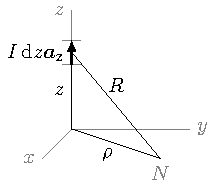
\includegraphics{figMagneticInfiniteStraightWiresDifferentialElement}
\caption{تار کے چھوٹے حصے سے پیدا سمتی مقناطیسی دباو۔}
\label{شکل_مقناطیسی_سمتی_مقناطیسی_دباو_تفرق_حصہ}
\end{figure}

شکل \حوالہ{شکل_مقناطیسی_سمتی_مقناطیسی_دباو_تفرق_حصہ} میں \عددیء{z} محدد پر لامحدود لمبائی کے برقی رو گزارتے تار کا چھوٹا حصہ \عددیء{\dif \kvec{L}} دکھایا گیا ہے۔نقطہ \عددیء{N} پر یہ
\begin{align*}
\dif \kvec{A}=\frac{\mu_0 I \dif z \az}{4\pi \sqrt{\rho^2+z^2}}
\end{align*}
یا
\begin{align}
\dif  A_z=\frac{\mu_0 I \dif z}{4\pi \sqrt{\rho^2+z^2}} \,\, , \quad \dif A_\rho=0, \quad \dif A_\phi=0
\end{align}
سمتی مقناطیسی دباو پیدا کرے گا۔آپ دیکھ سکتے ہیں کہ تار کے ہر چھوٹے حصے کا پیدا کردہ سمتی مقناطیسی دباو تار کے اسی حصے کی سمت میں ہو گا۔

مقناطیسی شدت  نلکی محدد میں مندرجہ بالا مساوات کے گردش
\begin{align*}
\dif \kvec{H}=\frac{1}{\mu_0} \nabla \times \dif \kvec{A}&=\frac{1}{\mu_0} \left(-\frac{\partial \dif A_z}{\partial \rho} \right)\aphi\\
&=\frac{I \dif z}{4\pi} \frac{\rho \aphi}{\left(\rho^2+z^2 \right)^{\frac{3}{2}}}
\end{align*}
 سے حاصل ہو گا۔یہی مساوات شکل \حوالہ{شکل_مقناطیسی_سمتی_مقناطیسی_دباو_تفرق_حصہ} کو دیکھتے ہوئے بایوٹ سیوارٹ کے مساوات سے لکھی جا سکتی ہے۔

سمتی مقناطیسی دباو \عددیء{\kvec{A}} کے کلیات دیگر اشکال کے کثافت برقی رو کے لئے بھی لکھا جا سکتے ہیں۔یوں سطحی کثافت برقی رو \عددیء{\kvec{K}} کے لئے  برقی رو کے چھوٹے حصے کو
\begin{align*}
I \dif \kvec{L}=\kvec{K} \dif S
\end{align*}
اور حجمی کثافت برقی رو \عددیء{\kvec{J}} کے لئے
\begin{align*}
I \dif \kvec{L}=\kvec{J} \dif h
\end{align*}
لکھے جا سکتے ہیں۔ لکیری برقی رو کے چھوٹے حصے کو عموماً \عددیء{I \dif \kvec{L}} لکھا جاتا ہے۔یوں برقی رو کو غیر سمتی تصور کرتے ہوئے فاصلے کو سمتی تصور کیا جاتا ہے۔اس کے برعکس مندرجہ بالا دو مساوات میں کثافت برقی رو کو سمتی مقدار تصور کیا گیا جبکہ تفرقی سطح \عددیء{\dif S} اور تفرقی حجم \عددیء{\dif h} کو غیر سمتی تصور کیا گیا۔یوں \عددیء{\kvec{A}} کے دیگر کلیے 
\begin{align}
\kvec{A}=\int_S \frac{\mu_0 \kvec{K} \dif S}{4\pi R}
\end{align}
اور
\begin{align}\label{مساوات_مقناطیسی_سمتی_مقناطیسی_دباو_حجمی_رو}
\kvec{A}=\int_h \frac{\mu_0 \kvec{J} \dif h}{4\pi R}
\end{align}
ہیں۔ 

سمتی مقناطیسی دباو مختلف اشکال کے برقی رو اور کثافت برقی رو سے مندرجہ بالا مساوات کی مدد سے حاصل ہوتے ہیں۔برقی دباو کی طرح سمتی مقناطیسی دباو کا زمین بھی لامحدود فاصلے پر رکھا جاتا ہے یعنی \عددیء{R \to \infty} پر \عددیء{\kvec{A} \to 0} تصور کیا جاتا ہے۔لامحدود فاصلے پر کوئی بھی برقی رو \عددیء{R \to \infty} کی بنا پر سمتی مقناطیسی دباو پر کوئی اثر نہیں ڈال سکتا۔
%===============

\ابتدا{مثال}
رداس \عددیء{a} کے موصل تار میں یکساں برقی رو \عددیء{I} گزر رہی ہے۔تار کے اندر \عددیء{\kvec{B}} حاصل کرتے ہوئے \عددیء{\kvec{A}} بھی حاصل کریں۔

حل:تار کو \عددیء{z} محدد پر پڑا تصور کرتے ہیں۔تار کے اندر \عددیء{\rho} رداس کا بند دائرہ \عددیء{\tfrac{I \pi \rho^2}{\pi a^2}} برقی رو گھیرے گی لہٰذا اس دائرے پر \عددیء{\kvec{B}=\tfrac{\mu_0 I \rho}{2\pi a^2}\aphi} ہو گا۔آپ دیکھ سکتے ہیں کہ \عددیء{\kvec{B}} کا صرف زاویائی جزو پایا جاتا ہے۔یوں \عددیء{\kvec{A}} کے گردش کو مساوات \حوالہ{مساوات_مقناطیسی_نلکی_محدد_میں_گردش} کی مدد سے لکھتے ہوئے صرف زاویائی جزو لیتے ہیں۔اس طرح
\begin{align*}
B_{\phi}=\frac{\partial A_\rho}{\partial z}-\frac{\partial A_z}{\partial \rho}
\end{align*} 
لکھا جا سکتا ہے۔چونکہ برقی رو  \عددیء{\az} سمت میں ہے لہٰذا \عددیء{\kvec{A}} کا صرف \عددیء{A_z} جزو متوقع ہے لہٰذا مندرجہ بالا مساوات 
\begin{align*}
B_{\phi}=-\frac{\partial A_z}{\partial \rho}
\end{align*} 
یعنی
\begin{align*}
-\frac{\partial A_z}{\partial \rho}=\frac{\mu_0 I \rho}{2\pi a^2}
\end{align*}
صورت  اختیار کر لے گا جس سے
\begin{align*}
A_z= \tfrac{\mu_0 I \rho^2 }{4\pi a^2} +M
\end{align*}
حاصل ہوتا ہے جہاں \عددیء{M} تکمل کا مستقل ہے۔
\انتہا{مثال}
%=================

\حصہ{ساکن مقناطیسی میدان کے قوانین کا حصول}
ساکن مقناطیس میدان کے تمام قوانین بایوٹ سیوارٹ کے قانون،
\begin{align}\label{مساوات_مقناطیسی_بایوٹ_سیوارٹ_قانون_بطور_ثبوت}
\kvec{H}=\oint \frac{I \dif \kvec{L} \times \aR}{4\pi R^2}
\end{align}
سمتی مقناطیسی دباو کے تعریف
\begin{align}\label{مساوات-مقناطیسی_سمتی_مقناطیسی_دباو_تعریف_دوبارہ}
\kvec{B}=\nabla \times \kvec{A}
\end{align}
اور مقناطیسی میدان کی شدت اور کثافت مقناطیسی  بہاو کے تعلق
\begin{align}\label{مساوات_مقناطیسی_شدت_اور_کثافت_بہاو_کا_تعلق}
\kvec{B}=\mu_0 \kvec{H}
\end{align}
سے حاصل کئے جا سکتے ہیں۔آئیں ایسا ہی کرتے  ہیں۔امید کی جاتی ہے کہ طلبہ و طالبات مندرجہ ذیل ثبوت کو سمجھتے ہوئے پڑھیں گے۔آپ سے گزارش کی جاتی ہے کہ انہیں یاد کرنے کی کوشش نہ کریں۔

\جزوحصہ{سمتی مقناطیسی دباو}\شناخت{حصہ_مقناطیسی_سمتی_مقناطیسی_دباو_ثبوت}
سمتی مقناطیسی دباو \عددیء{\kvec{A}} کی مساوات
\begin{align}\label{مساوات_مقناطیسی_سمتی_مقناطیسی_دباو_حجمی_رو_ب}
\kvec{A}=\int_h \frac{\mu_0 \kvec{J} \dif h}{4\pi R}
\end{align}
ثابت کرنے کی خاطر ہم اس سے بایوٹ سیوارٹ کا قانون یعنی مساوات  \حوالہ{مساوات_مقناطیسی_بایوٹ_سیوارٹ_قانون_بطور_ثبوت} حاصل کرتے ہیں۔مساوات \حوالہ{مساوات_مقناطیسی_سمتی_مقناطیسی_دباو_حجمی_رو} میں \عددیء{(x_2,y_2,z_2)} پر سمتی مقناطیسی دباو دی گئی ہے جبکہ \عددیء{(x_1,y_1,z_1)} وہ مقام ہے جہاں برقی رو گزارتا تار کا چھوٹا حصہ پایا جاتا ہے۔یوں چھوٹے حجم کو \عددیء{\dif h_1} لکھیں گے جو \عددیء{\dif x_1 \dif y_1 \dif z_1} کے برابر ہو گا۔تکمل کے متغیرات \عددیء{x_1}، \عددیء{y_1} اور \عددیء{z_1} ہیں۔یوں
\begin{align}\label{مساوات_مقناطیسی_سمتی_مقناطیسی_دباو_دوسرا_نقطہ}
\kvec{A}_2=\int_h \frac{\mu_0 \kvec{J}_1 \dif h_1}{4\pi R_{21}}
\end{align}
لکھا جا سکتا ہے۔اب 
\begin{align*}
\kvec{H}_2=\frac{\kvec{B}_2}{\mu_0}=\frac{\nabla_2 \times \kvec{A}_2}{\mu_0}
\end{align*}
کے برابر ہے جہاں \عددیء{\nabla_2} کے زیر نوشت میں \عددیء{2} لکھ کر یاد دہانی کرائی گئی ہے کہ گردش نقطہ \عددیء{(x_2,y_2,z_2)} پر حاصل کیا جائے گا لہٰذا گردش کے متغیرات بھی \عددیء{x_2}، \عددیء{y_2} اور \عددیء{z_2} ہی ہوں گے۔آپ کو یاد ہو گا کہ صفحہ \حوالہصفحہ{مثال_توانائی_ڈھلوان_مختلف_نقطوں_کے_متغیرات_کے_ساتھ} پر مثال \حوالہ{مثال_توانائی_ڈھلوان_مختلف_نقطوں_کے_متغیرات_کے_ساتھ} میں ڈھلوان حاصل کرتے ہوئے بالکل اسی طرح کیا گیا تھا۔یوں موجودہ مسئلے میں گردش حاصل کرتے وقت تمام تفرق \عددیء{x_2}، \عددیء{y_2} اور \عددیء{z_2} کے ساتھ لئے جائیں گے۔

اس طرح مساوات \حوالہ{مساوات_مقناطیسی_سمتی_مقناطیسی_دباو_دوسرا_نقطہ} سے \عددیء{\kvec{A}_2} پر کرتے ہوئے
\begin{align*}
\kvec{H}_2=\frac{1}{\mu_0} \nabla_2 \times \int_h \frac{\mu_0 \kvec{J}_1 \dif h_1}{4\pi R_{21}}
\end{align*}
حاصل ہوتا ہے۔گردش  بنیادی طور پر تفرق کا عمل ہے۔اس مساوات میں تکمل کا گردش حاصل کیا جا رہا ہے۔تکمل اور تفرق جس ترتیب سے حاصل کئے جائیں، اس کا حاصل جواب پر کوئی اثر نہیں ہے لہٰذا ہم تفرق کے عمل کو تکمل کے اندر لے جا سکتے ہیں جبکہ \عددیء{\tfrac{\mu_0}{4\pi}} مستقل ہے جسے تکمل کے باہر لایا جا سکتا ہے۔یوں
\begin{align*}
\kvec{H}_2=\frac{1}{4\pi}  \int_h \nabla_2 \times\frac{ \kvec{J}_1 \dif h_1}{ R_{21}}
\end{align*}
لکھا جا سکتا ہے۔یہاں \عددیء{\dif h_1=\dif x_1 \dif y_1 \dif z_1} پہلے تو مقداری ہے جس کی گردش حاصل نہیں کی جا سکتی۔ اس کے علاوہ اس کا \عددیء{x_2}، \عددیء{y_2} اور \عددیء{z_2} کے ساتھ تفرق صفر کے برابر ہے لہٰذا اسے گردش کے عمل سے  باہر لکھا جا سکتا ہے یعنی
\begin{align}\label{مساوات_مقناطیسی_گردش_ثبوت_الف}
\kvec{H}_2=\frac{1}{4\pi}  \int_h \left(\nabla_2 \times\frac{ \kvec{J}_1}{ R_{21}}\right) \dif h_1
\end{align}
یہاں سمتیہ \عددیء{\kvec{J}} ضرب مقداری \عددیء{\tfrac{1}{R_{21}}} کا گردش لیا جا رہا ہے۔مثال \حوالہ{مثال_مقناطیسی_سمتیہ_ضرب_مقداری_کی_گردش} میں کسی بھی سمتیہ \عددیء{\kvec{S}} اور مقداری \عددیء{M} کے حاصل ضرب کی گردش
\begin{align}
\nabla \times (M \kvec{S}) \equiv (\nabla M) \times \kvec{S} +M(\nabla \times \kvec{S})
\end{align}
حاصل کی گئی۔اس کی مدد سے مساوات \حوالہ{مساوات_مقناطیسی_گردش_ثبوت_الف} کو کھولتے ہیں جہاں سمتیہ \عددیء{\kvec{J}_1} اور مقداری \عددیء{\tfrac{1}{R_{21}}} ہیں۔
\begin{align}\label{مساوات_مقناطیسی_گردش_ثبوت_ب}
\kvec{H}_2=\frac{1}{4\pi}  \int_h  \left[ \left(\nabla_2 \frac{1}{R_{21}}\right) \times \kvec{J}_1 +\frac{1}{R_{21}} (\nabla_2 \times \kvec{J}_1) \right]\dif h_1
\end{align}
اس مساوات کے دوسرے جزو میں \عددیء{\kvec{J}_1} صرف \عددیء{x_1}، \عددیء{y_1} اور \عددیء{z_1} پر منحصر ہے۔نقطہ \عددیء{(x_2,y_2,z_2)} کا اس پر کسی قسم  کا کوئی اثر نہیں لہٰذا \عددیء{\kvec{J}_1} کے تمام تفرق جو \عددیء{x_2}، \عددیء{y_2} اور \عددیء{z_2} کے ساتھ لئے جائیں صفر کے برابر ہوں گے۔یوں \عددیء{\nabla_2 \times \kvec{J}_1=0} ہو گا۔

صفحہ \حوالہصفحہ{مساوات_توانائی_فاصلہ_ڈھلوان} پر مساوات \حوالہ{مساوات_توانائی_فاصلہ_ڈھلوان} کے استعمال سے مندرجہ بالا مساوات
\begin{align*}
\kvec{H}_2=-\frac{1}{4\pi}  \int_h \frac{\kvec{a}_{R21} \times \kvec{J}_1}{R_{21}^2}\dif h_1
\end{align*}
یا
\begin{align*}
\kvec{H}_2=\frac{1}{4\pi}  \int_h \frac{\kvec{J}_1 \times \kvec{a}_{R21} }{R_{21}^2}\dif h_1
\end{align*}
لکھی جا سکتی ہے۔اس میں \عددیء{\kvec{J}_1 \dif h_1} کی جگہ لکیری انداز میں \عددیء{I_1 \dif \kvec{L}_1} پر کرتے ہوئے اور بند تکمل لکھ کر جانی پہچانی بایوٹ سیوارٹ مساوات
\begin{align*}
\kvec{H}_2= \oint_h \frac{I \dif \kvec{L}_1 \times \kvec{a}_{R21} }{4\pi R_{21}^2}
\end{align*}
حاصل ہوتی ہے۔یوں ثابت ہوتا ہے کہ مساوات \حوالہ{مساوات_مقناطیسی_سمتی_مقناطیسی_دباو_دوسرا_نقطہ} درست ہے اور یہ مساوات \عددیء{مساوات_مقناطیسی_بایوٹ_سیوارٹ_قانون_بطور_ثبوت}، مساوات \عددیء{مساوات-مقناطیسی_سمتی_مقناطیسی_دباو_تعریف_دوبارہ} اور مساوات \عددیء{مساوات_مقناطیسی_شدت_اور_کثافت_بہاو_کا_تعلق} پر پورا اترتا ہے۔

\جزوحصہ{ایمپیئر کا دوری قانون}\شناخت{حصہ_ایمپیئر_کا-دوری_قانون}

آئیں اب ایمپیئر کے دوری قانون کی نقطہ شکل
\begin{align}
\nabla \times \kvec{H}=\kvec{J}
\end{align}
کو بایوٹ سیوارٹ کے قانون سے حاصل کریں۔

شروع کرتے ہیں مساوات \حوالہ{مساوات-مقناطیسی_سمتی_مقناطیسی_دباو_تعریف_دوبارہ} اور مساوات \حوالہ{مساوات_مقناطیسی_شدت_اور_کثافت_بہاو_کا_تعلق} سے جن سے
\begin{align}
\nabla \times \kvec{H}=\nabla \times \frac{\kvec{B}}{\mu_0}=\frac{1}{\mu_0} \nabla \times \nabla \times \kvec{A}
\end{align}
لکھا جا سکتا ہے۔صفحہ \حوالہصفحہ{مساوات_مقناطیسی_گردش_کی_گردش_ب} پر مساوات \حوالہ{مساوات_مقناطیسی_گردش_کی_گردش_ب} استعمال کرتے ہوئے یوں
\begin{align}\label{مساوات_مقناطیسی_مقناطیسی_میدان_کے_شدت_کی_گردش}
\nabla \times \kvec{H}=\frac{1}{\mu_0} \left[\nabla \left(\nabla \cdot \kvec{A} \right)-\nabla^2 \kvec{A} \right]
\end{align}
لکھا جا سکتا ہے۔مندرجہ بالا مساوات میں پھیلاو اور لاپلاسی کے عمل درکار ہیں۔

پھیلاو کو پہلے حل کرتے ہیں۔مساوات \حوالہ{مساوات_مقناطیسی_سمتی_مقناطیسی_دباو_دوسرا_نقطہ} کی پھیلاو
\begin{align}
\nabla_2 \cdot \kvec{A}_2=\frac{\mu_0}{4\pi}\int_h \nabla_2 \cdot \frac{\kvec{J}_1}{R_{21}} \dif h_1
\end{align}
لکھی جا سکتی ہے۔صفحہ \حوالہصفحہ{مثال_توانائی_توانائی_ضرب_برقی_بہاو_کی_ڈھلوان} پر مثال \حوالہ{مثال_توانائی_توانائی_ضرب_برقی_بہاو_کی_ڈھلوان} میں سمتیہ \عددیء{\kvec{D}} اور مقداری \عددیء{V} کے لئے
\begin{align*}
\nabla \cdot  (V \kvec{D})=V (\nabla \cdot \kvec{D})+\kvec{D} \cdot (\nabla V)
\end{align*}
ثابت کیا گیا۔یہاں سمتیہ \عددیء{\kvec{J}_1} جبکہ مقداری \عددیء{\tfrac{1}{R_{21}}} ہیں لہٰذا اس مساوات کو یوں لکھا جا سکتا ہے
\begin{align}\label{مساوات_مقناطیسی_سمتیہ_اور_مقداری_کے_حاصل_ضرب_کی_گردش_ب}
\nabla \cdot  \left(\frac{ \kvec{J}_1}{R_{21}}\right)=\frac{1}{R_{21}} (\nabla \cdot \kvec{J}_1)+\kvec{J}_1 \cdot \left(\nabla \frac{1}{R_{21}}\right)
\end{align}
 جس کی مدد سے
\begin{align}
\nabla_2 \cdot \kvec{A}_2=\frac{\mu_0}{4\pi}\int_h \left[\frac{1}{R_{21}} (\nabla_2 \cdot \kvec{J}_1)+\kvec{J}_1 \cdot \left(\nabla_2 \frac{1}{R_{21}}\right)\right] \dif h_1
\end{align}
ہو گا۔

چونکہ \عددیء{\kvec{J}_1} صرف متغیرات \عددیء{x_1}، \عددیء{y_1} اور \عددیء{z_1} پر منحصر ہے لہٰذا اس کے \عددیء{x_2}، \عددیء{y_2} اور \عددیء{z_2} کے ساتھ تفرق صفر کے برابر ہوں گے لہٰذا \عددیء{\nabla_2 \cdot  \kvec{J}_1=0} ہو گا۔

ہم صفحہ \حوالہصفحہ{مساوات_توانائی_فاصلے_کی_ڈھلوان_ب} پر مساوات \حوالہ{مساوات_توانائی_فاصلے_کی_ڈھلوان_ب}
\begin{align*}
\nabla_1 \frac{1}{R_{21}}=-\nabla_2 \frac{1}{R_{21}}
\end{align*}
کو استعمال کرتے ہوئے یوں 
\begin{align}
\nabla_2 \cdot \kvec{A}_2=\frac{\mu_0}{4\pi}\int_h \left[-\kvec{J}_1 \cdot \left(\nabla_1 \frac{1}{R_{21}}\right)\right] \dif h_1
\end{align}
لکھ سکتے ہیں۔مساوات \حوالہ{مساوات_مقناطیسی_سمتیہ_اور_مقداری_کے_حاصل_ضرب_کی_گردش_ب} کے دوبارہ استعمال سے 
\begin{align}
\nabla_2 \cdot \kvec{A}_2=\frac{\mu_0}{4\pi}\int_h \left[\frac{1}{R_{21}} (\nabla_1 \cdot \kvec{J}_1)-\nabla_1 \cdot \left(\frac{\kvec{J}_1}{R_{21}} \right)\right] \dif h_1
\end{align}
حاصل ہوتا ہے۔مساوات \حوالہ{مساوات_مقناطیسی_استمراری_مساوات} کہتی ہے کہ ساکن مقناطیسی میدان صرف اس صورت پیدا ہو گا جب \عددیء{\nabla \cdot \kvec{J}=0} ہو۔چونکہ ہمیں ساکن مقناطیسی میدان سے ہی غرض ہے لہٰذا مندرجہ بالا مساوات میں سے
\begin{align}
\nabla_2 \cdot \kvec{A}_2=-\frac{\mu_0}{4\pi}\int_h \nabla_1 \cdot \left(\frac{\kvec{J}_1}{R_{21}} \right) \dif h_1
\end{align}
حاصل ہوتا ہے۔صفحہ \حوالہصفحہ{مساوات_گاوس_مسئلہ_پھیلاو_تکمل_شکل} پر مساوات \حوالہ{مساوات_گاوس_مسئلہ_پھیلاو_تکمل_شکل} مسئلہ پھیلاو بیان کرتا ہے جس کے تحت حجمی تکمل کو سطحی تکمل کی صورت میں لکھا جا سکتا ہے۔اسے استعمال کرتے ہوئے یوں
\begin{align}
\nabla_2 \cdot \kvec{A}_2=-\frac{\mu_0}{4\pi}\oint_{S_1} \frac{\kvec{J}_1}{R_{21}} \cdot \dif \kvec{S}_1
\end{align}
حاصل ہوتا ہے جہاں سطح \عددیء{S_1} اس تمام حجم کو گھیرتی ہے جس پر حجمی تکمل حاصل کیا گیا تھا۔چونکہ حجمی تکمل اس غرض سے حاصل کیا گیا تھا کہ ساکن مقناطیسی میدان پیدا کرنے والے برقی رو کو مکمل طور پر شامل کیا جائے  لہٰذا اس حجم کے باہر کسی قسم کا کوئی برقی رو نہیں پایا جاتا۔اگر حجم سے باہر کوئی بھی برقی رو ہوتی تب ہمیں حجم کو بڑھا کر اس برقی رو کے اثر کو بھی شامل کرنا ہوتا۔ہم تکمل لیتے ہوئے حجم کو مزید بڑھا سکتے ہیں تا کہ اس کی سطح کو برقی رو نہ چھوئے۔ہم ایسا اس لئے کر سکتے ہیں کہ برقی رو سے خالی حجم کے شمول سے تکمل کی قیمت تبدیل نہیں ہوتی۔یوں ضرورت سے زیادہ حجم پر تکمل سے مراد یہ بھی ہے کہ سطحی تکمل ایسی سطح پر لی جائے جس پر کثافت برقی رو صفر کے برابر ہو۔صفر کثافت برقی رو کا سطحی تکمل صفر کے برابر ہوتا ہے لہٰذا مندرجہ بالا مساوات سے
\begin{align}\label{مساوات_مقناطیسی_سمتی_مقناطیسی_دباو_کی_پھیلاو_صفر_ہے}
\nabla \cdot \kvec{A}=0
\end{align}
حاصل ہوتا ہے جو کہتا ہے کہ سمتی مقناطیسی دباو کا پھیلاو صفر کے برابر ہے۔اس مساوات میں زیر نوشت میں \عددیء{2} نہیں لکھا گیا ہے جو اس نقطے کی نشاندہی کرتا ہے جہاں مقناطیسی میدان کی بات ہو رہی ہو۔پھیلاو بھی اسی نقطے پر حاصل کیا جاتا ہے۔یاد رہے کہ ہم مساوات \حوالہ{مساوات_مقناطیسی_مقناطیسی_میدان_کے_شدت_کی_گردش} حل کرنے کی خاطر پھیلاو اور لاپلاسی حاصل کرنے نکلے تھے۔پھیلاو حاصل ہو چکا ہے آئیں اب لاپلاسی حاصل کریں۔  

برقی دباو اور سمتی مقناطیسی دباو کے ایک جزو
\begin{align*}
V&=\int_h \frac{\rho \dif h}{4\pi \epsilon_0 R}\\
A_x&=\int_h \frac{\mu_0 J_x \dif h}{4\pi R}
\end{align*}
 کا موازنہ کرنے سے صاف ظاہر ہے کہ \عددیء{\rho} اور \عددیء{J_x} کو آپس میں تبدیل کرتے ہوئے اور \عددیء{\tfrac{1}{\epsilon_0}} اور \عددیء{\mu_0} کو آپس میں تبدیل کرتے ہوئے ایک مساوات سے دوسری مساوات حاصل کی جا سکتی ہے۔اب ہم پوئسن  مساوات
\begin{align*}
\nabla^2 V=-\frac{\rho}{\epsilon_0}
\end{align*} 
میں یہی تبدیلیاں کرتے ہوئے
\begin{align*}
\nabla^2 A_x=-\mu_0 J_x
\end{align*}
اور
\begin{align*}
\nabla^2 A_y&=-\mu_0 J_y\\
\nabla^2 A_z&=-\mu_0 J_z
\end{align*}
لکھ سکتے ہیں جنہیں یوں
\begin{align}\label{مساوات_مقناطیسی_سمتی_مقناطیسی_دباو_کی_لاپلاسی}
\nabla^2 \kvec{A}=-\mu_0 \kvec{J}
\end{align}
 بھی لکھا جا سکتا ہے۔

مساوات \حوالہ{مساوات_مقناطیسی_مقناطیسی_میدان_کے_شدت_کی_گردش} میں مساوات \حوالہ{مساوات_مقناطیسی_سمتی_مقناطیسی_دباو_کی_پھیلاو_صفر_ہے} اور مساوات \حوالہ{مساوات_مقناطیسی_سمتی_مقناطیسی_دباو_کی_لاپلاسی} استعمال کرتے ہوئے یوں ایمپیئر کے دوری قانون کی نقطہ شکل 
\begin{align}
\nabla \times \kvec{H}=\kvec{J}
\end{align}
حاصل ہوتی ہے۔
%========================

\ابتدا{مثال}
مندرجہ بالا حصے میں برقی دباو کے لاپلاسی سے سمتی مقناطیسی  دباو کی لاپلاسی اخذ کی گئی۔سمتی مقناطیسی دباو کے لاپلاسی کو ایمپیئر کے دوری قانون اور \عددیء{\kvec{A}} کی تعریف سے حاصل کریں۔

حل:ایمپیئر کے دوری قانون کی نقطہ شکل اور \عددیء{\kvec{A}} کی تعریف
\begin{align*}
\nabla \times \kvec{H}&=\kvec{J}\\
\kvec{B}&=\nabla \times \kvec{A}
\end{align*}
سے
\begin{align*}
\nabla \times \nabla \times \kvec{A}=\mu_0 \kvec{J}
\end{align*}
لکھا جا سکتا ہے جہاں \عددیء{\kvec{B}=\mu_0 \kvec{H}} کا استعمال کیا گیا ہے۔صفحہ \حوالہصفحہ{مساوات_مقناطیسی_گردش_کی_گردش_ب} پر مساوات \حوالہ{مساوات_مقناطیسی_گردش_کی_گردش_ب} استعمال کرتے ہوئے
\begin{align*}
\nabla \left(\nabla \cdot \kvec{A} \right)-\nabla^2 \kvec{A}=\mu_0 \kvec{J}
\end{align*}
حاصل ہوتا ہے جسے مساوات \حوالہ{مساوات_مقناطیسی_سمتی_مقناطیسی_دباو_کی_پھیلاو_صفر_ہے} کی مدد سے
\begin{align}
\nabla^2 \kvec{A}=-\mu_0 \kvec{J}
\end{align}
لکھا جا سکتا ہے۔
\انتہا{مثال}
%======================
\newpage
\حصہء{سوالات}
%=============================
\ابتدا{سوال}
لامحدود لمبائی کی سیدھی تار \عددی{y } محدد پر پڑی ہے۔اس میں \عددی{\ay} جانب \عددی{\SI{5}{\milli\ampere}} برقی رو گزر رہی ہے۔ نقطہ \عددی{N(2,5,3)} پر مقناطیسی میدان \عددی{\kvec{H}} اور \عددی{\abs{\kvec{H}}} حاصل کریں۔اگر تار \عددی{x=3}، \عددی{z=-1} پر ہو تب جوابات کیا ہوں گے۔دونوں تاروں کی موجودگی میں جوابات حاصل کریں۔ 

جوابات: \عددی{\kvec{H}=184\ax-122\az \, \si{\micro\ampere\per\meter}}، \عددی{\abs{\kvec{H}}=\SI{221}{\micro\ampere\per\meter}}، \عددی{\kvec{H}=187\ax+47\az \, \si{\micro\ampere\per\meter}}، \عددی{\abs{\kvec{H}}=\SI{193}{\micro\ampere\per\meter}}،\\
 \عددی{{\kvec{H}=371\ax-75\az \, \si{\micro\ampere\per\meter}}}، \عددی{\abs{\kvec{H}}=\SI{378}{\micro\ampere\per\meter}}
\انتہا{سوال}
%======================
\ابتدا{سوال}
مساوات \حوالہ{مساوات_مقناطیسی_محدود_تار_کی_مقناطیس} حاصل کریں۔
\انتہا{سوال}
%===============

\ابتدا{سوال}
سطح \عددی{z=0} پر \عددی{y} محدد کے متوازی لامحدود لمبائی کے آٹھ عدد تار پڑے ہیں جن میں \عددی{\ay} جانب \عددی{\SI{1}{\ampere}} برقی رو گزر رہی ہے۔یہ تار \عددی{y=-3.5}، \عددی{y=-2.5}، \عددی{\cdots}، \عددی{y=2.5}، \عددی{y=3.5} پر پائے جاتے ہیں۔نقطہ \عددی{(0,0,1)} اور \عددی{(0,0,50)} پر \عددی{\kvec{H}} حاصل کریں۔

جوابات: \عددی{0.421\ax}، \عددی{0.0254\ax}؛ محدد پر پچاس گنا دور میدان صرف سترہ گنا کم ہے۔
\انتہا{سوال}
%======================
\ابتدا{سوال}
چار میٹر لمبے تار کو چکور کی شکل دی جاتی ہے جس کا رقبہ \عددی{\SI{1}{\meter\squared}} ہے۔اس چکور کو \عددی{z=0} سطح پر رکھا جاتا ہے۔تار میں برقی رو \عددی{\SI{10}{\milli\ampere}} گزرنے کی صورت میں چکور کے وسط \عددی{N(0,0,0)} میں مقناطیسی میدان \عددی{H} حاصل کریں۔نقطہ \عددی{P(0,0,1)} پر بھی میدان حاصل کریں۔

جوابات:\عددی{\SI{9}{\milli\ampere\per\meter}}، \عددی{\SI{2.3}{\milli\ampere\per\meter}}
\انتہا{سوال}
%=======================
\ابتدا{سوال}
شکل \حوالہ{شکل_مقناطیسی_لامحدود_سطحی_برقی_رو} کے لامحدود سطح سے پیدا مقناطیسی میدان بایوٹ-سیوارٹ کے قانون کی مدد سے حاصل کریں۔
\انتہا{سوال}
%=============

\ابتدا{سوال}
ایک تار کو دائری شکل دے کر سطح \عددی{z=0} پر رکھا جاتا ہے۔دائرے کا رقبہ \عددی{\SI{1}{\meter\squared}} ہے۔تار میں \عددی{\SI{10}{\milli\ampere}} گزرنے کی صورت میں دائرے کے وسط \عددی{N(0,0,0)} میں مقناطیسی میدان \عددی{H} حاصل کریں۔نقطہ \عددی{P(0,0,1)} پر بھی میدان حاصل کریں۔

جوابات: \عددی{\SI{2.82}{\milli\ampere\per\meter}}، \عددی{\SI{1.86}{\milli\ampere\per\meter}}
\انتہا{سوال}
%========================
\ابتدا{سوال}
محدد \عددی{x} اور \عددی{y} میں بڑھتے جانب \عددی{\SI{55}{\milli\ampere}} برقی رو گزر رہی ہے۔نقطہ \عددی{N(5,6,4)} پر \عددی{\kvec{H}} حاصل کریں۔

جواب:\عددی{854\ax-673\ay-57\az \, \si{\micro\ampere\per\meter}}
\انتہا{سوال}
%=======================
\ابتدا{سوال}
مساوات \حوالہ{مساوات_مقناطیسی_راہ_پہلے_حصے_پر_شدت_دوبارہ} حاصل کرنے کے طرز پر شکل \حوالہ{شکل-مقناطیسی_گردش_تعریف} میں \عددیء{3} تا \عددیء{4} پر \عددیء{H_{y34}} حاصل کریں۔

جواب:شرح \عددیء{\tfrac{\partial H_y}{\partial x}} ہے۔یوں \عددیء{-\tfrac{\Delta x}{2}} تبدیلی سے  \عددیء{\tfrac{\partial H_y}{\partial x}(-\frac{\Delta x}{2})} تبدیلی رو نما ہو گی اور یوں نئی قیمت 
{\عددیء{H_{y0}-\tfrac{\partial H_y}{\partial x}\tfrac{\Delta x}{2}}} ہو گی۔

\انتہا{سوال}
%===========
\ابتدا{سوال}
عمومی محدد میں حاصل کردہ گردش کی مساوات سے کارتیسی محدد میں گردش کی مساوات حاصل کریں۔
\انتہا{سوال}
%==============================

\ابتدا{سوال}
سطحی رو \عددی{\kvec{K}=\tfrac{8}{\rho}\aphi \, \si{\ampere\per\meter}} خطہ \عددی{\rho=\SI{3}{\meter}} تا \عددی{\rho=\SI{7}{\meter}} میں پائی جاتی ہے۔سطح \عددی{\phi=0} سے گزرتی کل برقی رو حاصل کریں۔نقطہ \عددی{N(0,0,z)} پر \عددی{\kvec{H}} حاصل کرتے ہوئے میدان کی قیمت \عددی{z=10} پر دریافت کریں۔

جوابات: \عددی{I=8\ln \tfrac{7}{3} \, \si{\ampere}}، \عددی{\kvec{H}=\left[\tfrac{4}{\sqrt{z^2+3^2}}-\tfrac{4}{\sqrt{z^2+7^2}}\right]\, \az}، \عددی{\SI{55.4}{\milli\ampere\per\meter}}
\انتہا{سوال}
%======================
\ابتدا{سوال}
سطحی رو \عددی{\kvec{K}=8\rho\aphi \, \si{\ampere\per\meter}} خطہ \عددی{\rho=\SI{3}{\meter}} تا \عددی{\rho=\SI{7}{\meter}} میں پائی جاتی ہے۔سطح \عددی{\phi=0} سے گزرتی کل برقی رو حاصل کریں۔نقطہ \عددی{N(0,0,z)} پر \عددی{\kvec{H}} حاصل کرتے ہوئے میدان کی قیمت \عددی{z=10} پر دریافت کریں۔

جوابات:\عددی{I=\SI{160}{\ampere}}، \عددی{\kvec{H}=4\left[\tfrac{2z^2+49}{\sqrt(z^2+49)}-\tfrac{2z^2+9}{\sqrt{z^2+9}}\right]\, \az}، \عددی{\SI{1.52}{\ampere\per\meter}}
\انتہا{سوال}
%==========================

\ابتدا{سوال}
عمومی محدد میں حاصل کردہ گردش کی مساوات سے نلکی محدد میں گردش کی مساوات حاصل کریں۔
\انتہا{سوال}
%==========

\ابتدا{سوال}
رداس \عددی{a} کے دائری چادر پر یکساں سطحی کثافت بار \عددی{\rho_S} پائی جاتی ہے۔چادر کے محور کو محدد کے مرکز پر رکھتے ہوئے چادر کو سطح \عددی{z=0} پر رکھا جاتا ہے۔اگر چادر محور کے گرد زاویائی رفتار \عددی{\omega} سے گھوم رہی ہو تب نقطہ \عددی{N(0,0,z)} پر مقناطیسی میدان \عددی{H} کیا ہو گا؟ میدان کی قیمت \عددی{\rho_S=\SI{5}{\micro\coulomb\per\meter\squared}} اور \عددی{\omega=100\pi \, \si{\radian\per\second}} کی صورت میں \عددی{(0,0,0.1)} پر حاصل کریں۔

جوابات: \عددی{\tfrac{\omega \rho_S}{2}\left[\tfrac{2z^2+4}{\sqrt{z^2+4}}-2z\right]}، \عددی{\SI{1.42}{\milli\ampere\per\meter}}
\انتہا{سوال}
%=======================
\ابتدا{سوال}
سطح \عددی{z=0} پر خطہ \عددی{x=\SI{-3}{\meter}} تا \عددی{x=\SI{3}{\meter}} پر سطحی برقی رو \عددی{\kvec{K}=4\ay \, \si{\ampere\per\meter}} پائی جاتی ہے۔نقطہ \عددی{N(0,0,5)} پر مقناطیسی میدان حاصل کریں۔

جواب:\عددی{0.688 \ax \, \si{\ampere\per\meter}}
\انتہا{سوال}
%========================
\ابتدا{سوال}
گول دائرے پر برقی رو کا دائرے کے محور سے ہٹ کر مقناطیسی میدان کی شدت حاصل کرتے ہوئے مساوات \حوالہ{مساوات_مقناطیسی_دائرے_کا_محور_سے_دور_اجزاء} میں دئے بیضوی تکمل حاصل کئے گئے۔ان میں \عددیء{H_y} کا عددی حل مثال \حوالہ{مثال_مقناطیسی_دائرہ_برقی_رو_کے_بیضوی_تکمل} میں حاصل کیا گیا۔بالکل اسی طرز پر تکمل کو دس ٹکڑوں میں کرتے ہوئے  \عددیء{H_z} کی عددی قیمت نقطہ \عددیء{N(0,a,a)} پر حاصل کریں۔

جواب:\عددیء{0.96525 \left(\tfrac{I}{4\pi a}\right)}
\انتہا{سوال}
%======================

\ابتدا{سوال}
سطح \عددی{x=0} پر سطحی برقی رو \عددی{1200\az \, \si{\ampere\per\meter}} پائی جاتی ہے۔خطہ \عددی{0<z<\infty}، \عددی{5<y<15} پر برقی رو سے نقطہ \عددی{N(10,0,0)} پر پیدا مقناطیسی میدان \عددی{\kvec{H}} حاصل کریں۔

جواب: \عددی{\kvec{H}=45.6\ax+49.6\ay \, \si{\ampere\per\meter}}
\انتہا{سوال}
%=======================
\ابتدا{سوال}
خطہ \عددی{0<z<5} میں یکساں کثافت برقی رو \عددی{15\ay \, \si{\ampere\per\meter\squared}} پائی جاتی ہے۔ایمپیئر  کے دوری قانون کی مدد سے ثابت کریں کہ \عددی{{\kvec{H}_{z<0}=-\kvec{H}_{z>5}}} کے برابر ہے۔نقطہ \عددی{(2,5,7)} اور نقطہ \عددی{(4,12,2)} پر \عددی{\kvec{H}} حاصل کریں۔

جوابات:\عددی{37.5 \ax \, \si{\ampere\per\meter}}، \عددی{-7.5\ax \, \si{\ampere\per\meter}}
\انتہا{سوال}
%=======================

\ابتدا{سوال}
محدد کے مرکز پر رداس \عددی{a} کا موصل کرہ پایا جاتا ہے۔منفی \عددی{z} محدد پر \عددی{10\az \, \si{\ampere}} کی برقی رو، کرہ کی سطح پر نقطہ \عددی{(0,0,-a)} تک پہنچتی ہے جہاں سے یہ کرہ کے سطح پر یکساں پھیل کر نقطہ \عددی{(0,0,a)} تک پہنچتی ہے اور اس کے بعد مثبت \عددی{z} محدد پر بڑھتے جانب چلے جاتی ہے۔کرہ کے اندر اور اس کے باہر مقناطیسی میدان حاصل کریں۔

جوابات:\عددی{\SI{0}{\ampere\per\meter}}، \عددی{\tfrac{10}{2\pi \rho} \aphi \, \si{\ampere\per\meter}}   
\انتہا{سوال}
%========================
\ابتدا{سوال}
منفی \عددی{z} محدد سے برقی رو \عددی{I} موصل  \عددی{\theta=30^{\circ}} سطح تک پہنچ کر سطح پر یکساں پھیل کر چلے جاتی ہے۔نقطہ \عددی{(0,0,z)} اور نقطہ \عددی{(5,5,5)} پر مقناطیسی میدان \عددی{H} حاصل کریں۔

جوابات: \عددی{\SI{0}{\ampere\per\meter}}، \عددی{\tfrac{I}{2\pi \sqrt{50}} \, \si{\ampere\per\meter}}
\انتہا{سوال}
%=========================
\ابتدا{سوال}\شناخت{سوال_مقناطیسی_میدان_گردش_جزو}
تفاعل \عددی{\kvec{G}=(5x+yz)\ax+3xyz\ay+\tfrac{x^2 y}{z}\az} نقطہ \عددی{N(0.6,0.4,0.2)} اور اس کے قریب پایا جاتا ہے۔سطح \عددی{z=0.2} پر \عددی{2a} لمبائی کے اطراف کے مربع لکیر پر \عددی{\oint \kvec{G} \cdot \dif \kvec{L}} حاصل کریں جہاں مربع کا مرکز نقطہ \عددی{N} پر ہے۔لکیری تکمل کو مربع کے رقبے سے تقسیم کریں اور \عددی{a \to 0} لیتے ہوئے \عددی{\nabla \times \kvec{G}_z} حاصل کریں۔

جوابات:چاروں اطراف کے لکیری تکمل \عددی{0.48a^2+0.288a}، \عددی{0.48a^2-0.288a}، \عددی{-0.4a^2+6.16a}  اور \عددی{-0.4a^2-6.16a} ہیں۔یوں \عددی{\nabla \times \kvec{G}_z=0.04} ہے۔
\انتہا{سوال}
%========================
\ابتدا{سوال}
مساوات \حوالہ{مساوات_مقناطیسی_کارتیسی_گردش_ب} استعمال کرتے ہوئے تفاعل \عددی{\kvec{G}=(5x+yz)\ax+3xyz\ay+\tfrac{x^2 y}{z}\az} کا نقطہ \عددی{N(0.6,0.4,0.2)} پر \عددی{\nabla \times \kvec{G}} حاصل کریں۔سوال \حوالہ{سوال_مقناطیسی_میدان_گردش_جزو} میں حاصل کئے گئے \عددی{\nabla \times \kvec{G}_z} کے ساتھ موازنہ کریں۔

جواب: \عددی{1.08\ax-2\ay+0.04\az}
\انتہا{سوال}
%====================

\ابتدا{سوال}
ہم محوری تار میں \عددی{\kvec{E}=3000 \rho^{1.3} \cos(\omega t -0.3z) \arho \, \si{\volt\per\meter}} پایا جاتا ہے۔تار میں \عددی{\nabla \times \kvec{E}} حاصل کریں۔

جواب:\عددی{900 \rho^{1.3}\sin(\omega t -0.3 z) \aphi}
\انتہا{سوال}
%=========================
\ابتدا{سوال}
میدان \عددی{V=5(x^2+y^2)} اور \عددی{V=10x^3+y^2+xz^4} کے لئے \عددی{\nabla^2 V} اور \عددی{\nabla \times \kvec{E}} حاصل کریں۔

جوابات:\عددی{20}، \عددی{0}، \عددی{60x+2+12xz^2}، \عددی{0}
\انتہا{سوال}
%=========================
\ابتدا{سوال}
میدان \عددی{\kvec{H}=x^2y^2z\ax-xy^2z^2\az} دیا گیا ہے۔مسئلہ سٹوکس کے دونوں اطراف باری باری استعمال کرتے ہوئے،  سطح \عددی{y=1} میں خطہ \عددی{{1<x<2}}، \عددی{{1<z<3}} سے \عددی{\ay} جانب گزرتی برقی رو حاصل کریں۔

جواب:\عددی{\SI{13.3}{\ampere}}
\انتہا{سوال}
%========================

\ابتدا{سوال}
میدان \عددی{\kvec{H}=\tfrac{2xy}{z^2}\ax-\tfrac{y^2}{z^2}\ay+x^2y^2\az} دیا گیا ہے۔سطح \عددی{x=0.5} میں خطہ \عددی{{1<y<2}}، \عددی{{2<z<3}} سے \عددی{\ax} جانب گزرتی برقی رو درکار ہے۔الف) برقی رو کو بذریعہ سطحی تکمل حاصل کریں۔ ب) برقی رو کو بذریعہ لکیری تکمل حاصل کریں

جواب:\عددی{\SI{0.426}{\ampere}}
\انتہا{سوال}
%========================
\ابتدا{سوال}
کروی محدد میں میدان \عددی{\kvec{H}=\tfrac{50r}{\sin\theta} \aphi} دیا گیا ہے۔مسئلہ سٹوکس کے دونوں اطراف باری باری استعمال کرتے ہوئے کروی خطہ \عددی{{r=0.2}}، \عددی{0<\phi<2\pi}، \عددی{0<\theta<60^{\circ}} سے گزرتی برقی رو حاصل کریں۔

جواب:\عددی{\SI{5.44}{\ampere}}
\انتہا{سوال}
%=======================
\ابتدا{سوال}
میدان \عددی{\kvec{H}=\tfrac{4r^2}{\sin \theta}\atheta+50r\sin\theta\aphi} دیا گیا ہے۔سطح \عددی{\theta=45^{\circ}} میں خطہ \عددی{0<\phi<2\pi}، \عددی{0<r<3} سے \عددی{\atheta} جانب گزرتی برقی رو حاصل کریں۔ 

جواب:\عددی{\SI{-1414}{\ampere}}
\انتہا{سوال}
%=======================
\ابتدا{سوال}
پاکستان میں کل زمینی مقناطیسی میدان \عددی{\SI{45}{\micro\tesla}} تا \عددی{\SI{50}{\micro\tesla}} پایا جاتا ہے جس کا افقی جزو اوسطاً \عددی{\SI{30}{\micro\tesla}} کے لگ بھگ ہے۔ایک تار جس میں \عددی{\SI{1}{\ampere}} کی برقی رو گزر رہی ہو، کتنے فاصلے پر زمینی میدان کے افقی جزو برابر مقناطیسی میدان پیدا کرے گی۔

جواب:\عددی{\SI{4.2}{\centi\meter}} 
\انتہا{سوال}
%=======================
\ابتدا{سوال}
بیس سنٹی میٹر لمبائی اور پانچ سنٹی میٹر رداس کا پیچدار لچھا جس میں برقی رو گزر رہی ہو میں مقناطیسی میدان \عددی{\kvec{H}=200\az \, \si{\ampere\per\meter}} پایا جاتا ہے۔نقطہ \عددی{N_1(0.02,0^{\circ},0.02)} اور \عددی{N_2(0.04,50^{\circ},0.06)} کے درمیان غیر سمتی مقناطیسی دباو \عددی{V_{m21}} حاصل کریں۔سمتی مقناطیسی دباو \عددی{\nabla \times \kvec{B}=\kvec{A}} سے حاصل کرتے ہوئے \عددی{\rho=0} پر \عددی{\kvec{A}=0} لیتے ہوئے انہیں دو نقطوں کے مابین \عددی{\kvec{A}_{21}} حاصل کریں۔یہ مساوات استعمال کرتے وقت \عددی{\kvec{A}} کا درست جزو اپنے علم سے چنیں۔

جوابات: \عددی{\SI{-8}{\ampere}}، \عددی{2.5\aphi \, \si{\micro\weber\per\meter}}
\انتہا{سوال}
%======================
\ابتدا{سوال}
نلکی کثافت برقی رو \عددی{50\az \, \si{\ampere\per\meter}} رداس \عددی{\rho=\SI{2}{\meter}} پر پائی جاتی ہے جبکہ رداس \عددی{\rho=\SI{4}{\meter}} پر \عددی{25\az \, \si{\ampere\per\meter}} اور رداس \عددی{\rho=\SI{5}{\meter}} پر \عددی{-40\az \, \si{\ampere\per\meter}} پائے جاتے ہیں۔زاویہ \عددی{\phi=0} پر \عددی{V_m=0} لیتے اور \عددی{\phi=180^{\circ}} کو رکاوٹ تصور کرتے ہوئے  نقطہ \عددی{N_1(3.5,60^{\circ},0)}  پر غیر سمتی مقناطیسی دباو \عددی{V_m} حاصل کریں۔

جوابات: \عددی{\SI{-66.6}{\ampere}}
\انتہا{سوال}
%=======================
\ابتدا{سوال}
سطح \عددی{z=0} پر تار \عددی{x=4} میں \عددی{\SI{0.2}{\ampere}} کی برقی رو \عددی{\ay} جانب پائی جاتی ہے جبکہ تار \عددی{x=-4} میں \عددی{\SI{0.2}{\ampere}} برقی رو \عددی{-\ay} جانب پائی جاتی ہے۔محدد کے مرکز پر \عددی{V_m=0} لیتے ہوئے \عددی{z} محدد پر غیر سمتی مقناطیسی دباو \عددی{V_m} حاصل کریں۔

جواب:\عددی{-\tfrac{0.2}{\pi}\tan^{-1} \tfrac{z}{4}\, \si{\ampere}}
\انتہا{سوال}
%=======================
